\documentclass[12pt]{niuthesis}
\usepackage[utf8]{inputenc}
\usepackage{graphicx}
\usepackage{amsmath}
\usepackage{physics}
\usepackage{caption}
\usepackage{subcaption}
\usepackage{multirow}
\usepackage{xcolor}
\usepackage{listings}
\usepackage{braket}
\usepackage{hyperref}
\usepackage{pdflscape}
\usepackage{soul}
\usepackage{setspace}


\usepackage{listings}
\usepackage{xcolor}


% OMIT FOR FINAL PRODUCT
\usepackage{lineno}
%\linenumbers

\definecolor{codegreen}{rgb}{0,0.6,0}
\definecolor{codegray}{rgb}{0.5,0.5,0.5}
\definecolor{codepurple}{rgb}{0.58,0,0.82}
\definecolor{backcolour}{rgb}{0.95,0.95,0.92}

\lstdefinestyle{mystyle}{
    backgroundcolor=\color{backcolour},   
    commentstyle=\color{codegreen},
    keywordstyle=\color{magenta},
    numberstyle=\tiny\color{codegray},
    stringstyle=\color{codepurple},
    basicstyle=\ttfamily\footnotesize,
    breakatwhitespace=false,         
    breaklines=true,                 
    captionpos=b,
    frame=single,                    
    keepspaces=true,                 
    numbers=left,                    
    numbersep=5pt,                  
    showspaces=false,                
    showstringspaces=false,
    showtabs=false,                  
    tabsize=2
}

\lstset{style=mystyle}

%%%%%%%%%%%%%%%%%%%%%%%%%%%%%%%%%%%%%%%%%%%%%%%%%%%%%%%%%%%%%%%%%%



\usepackage[hyperref,backend=biber,backref,sorting=none]{biblatex}
\addbibresource{main.bib}




\title{Optimization of derivation jobs and modernization of I/O integration tests for the ATLAS Experiment}
\author{Arthur C. Kraus}
\major{Physics}
\degree{Thesis}{M.S.}{Master of Science}
\degreedate{May}{2025}
\department{Department of Physics}
\director{Jahred Adelman}


\begin{document}


\begin{abstract}
The High-Luminosity LHC (HL-LHC) is a phase of the LHC that is expected to start toward the end of the decade. 
With this comes an increase in data taken per year that current software and computing infrastructure, including I/O, is being prepared to handle. 
The ATLAS experiment's Software Performance Optimization Team has areas in development to improve the Athena software framework that is scalable in performance and ready for wide-spread HL-LHC era data taking. 
One area of interest is optimization of derivation production jobs by improving derived object data stored to disk by about 4-5\% by eliminating the upper-limit on TTree basket buffers, at the expense of an increase in memory usage by about 11\%. 

%:
Athena and the software it depends on are updated frequently, and to synthesize changes cohesively there are scripts, unit tests, that run which test core I/O functionality. 
This thesis upgrades existing I/O unit tests to now exercise features exclusive to the xAOD Event Data Model (EDM) such as writing and reading object data from the previous EDM using transient and persistent data. 
These new unit tests also include and omit select dynamic attributes to object data during the component accumulator step. 
\end{abstract}

\begin{dedication}
% I'd like to dedicate this thesis to my brother, Joseph, and to my sister, Emily. To my parents, Joyce Kraus D.S.W and Art Kraus, who have sacrificed more than I will ever know. 

To all of the fluffy kitties. To all of the fluffy kitties. To all of the fluffy kitties. To all of
the fluffy kitties. 


\end{dedication}

\begin{acknowledgements}
% Many thanks to Jahred Adelman for bringing this project to me and having boundless patience. I'd like to thank Alaettin Serhan Mete, for helping me realize the learning curve is not as steep as anticipated. Thanks to Peter van Gemmeren for the wisdom imparted every step of the way. 

% I also want to thank the professors I studied under during this degree: Stephen Martin, Bela Erdyli, Andreas Glatz and Hector de la Torre Perez. Each of your patience and wisdom have helped me shape the 

% I have to thank the other students I met at NIU, as it was through their support I was able to rekindle my passion for collaborating with the brightest and kindest people one could want to work alongside.  

Here’s where you acknowledge folks who helped. Here’s where you acknowledge folks who helped. Here’s where you acknowledge folks who helped. Here’s where you acknowledge folks who helped.
\end{acknowledgements}
\MakeThesisPrologue



% 1. Introduction
% -- At most 1-3 pages
% -- no need to talk about everything, just a high
% -- level breakdown 

\chapter{Introduction}
\label{chap:Intro}
Particle physics is the branch of physics that studies the fundamental constituents of matter and the forces governing their interactions.  
The field started as studies in electromagnetism, radiation, and further developed with the discovery of the electron.
What followed was more experiments to search for new particles, new models to describe the results, and new search techniques which demanded more data.
The balance in resources for an experiment bottlenecks how much data can be taken, so steps need to be taken to identify interesting interactions and optimize the storage and processing of this data.
This thesis investigates software performance optimization of the ATLAS experiment at CERN. 
Specifically, ways to modernize and optimize areas of the software framework, Athena, to improve input/output (I/O) performance during derivation production and create new tests that catch when specific core I/O functionality is broken.

\section{LHC and The ATLAS Detector}

\begin{figure}[h]
    \centering
    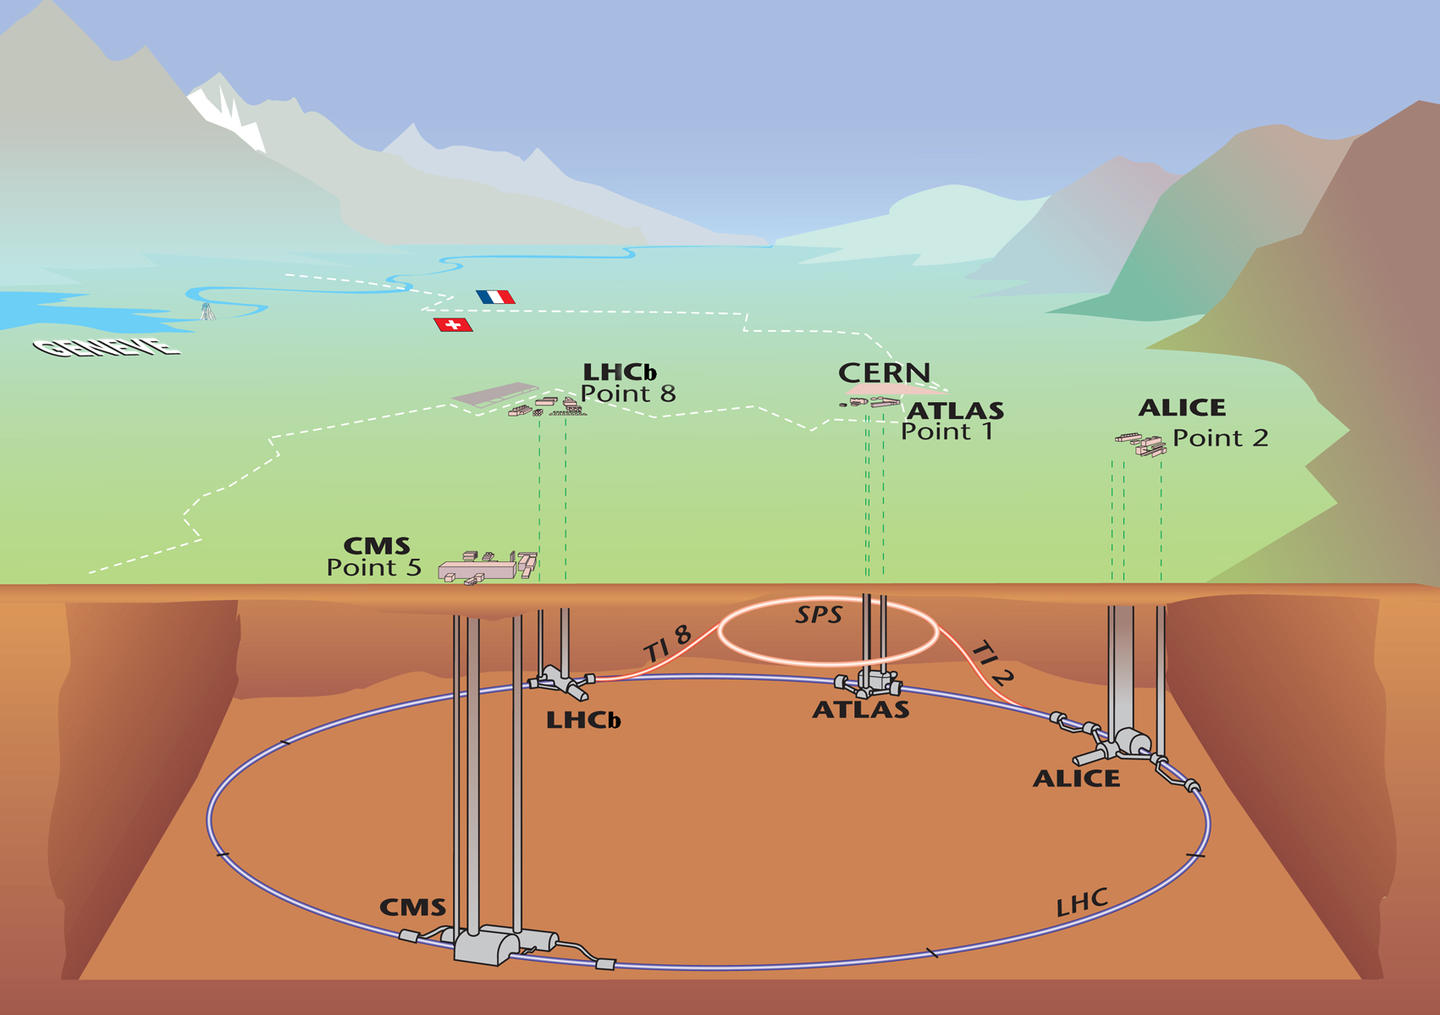
\includegraphics[width=.8\textwidth]{content/img/LHC illustration.jpg}
    \caption{Illustration of the LHC experiment sites on the France-Switzerland border.\cite{LHC_Illustration}}
    \label{fig:intro_LHC_sites}
\end{figure}

The Large Hadron Collider (LHC), shown in Figure \ref{fig:intro_LHC_sites},  is a particle accelerator spanning a 26.7-kilometer ring that crosses between the France-Switzerland border at a depth between 50 and 175 meters underground.\cite{Bruning:782076}
The ATLAS experiment, shown in Figure \ref{fig:intro_ATLAS_detector}, is the largest LHC general purpose detector, and the largest detector ever made for particle collision experiments. 
The detector lies in a cavern 92.5 m underground at a length of 46 m, height and width of 25 m.\cite{ATLAS_Tech_Proposal}
A quadrant of the detector is shown in Figure \ref{fig:ATLAS_quadrant}, where $\eta$ is a measure of the pseudo-rapidity.
Pseudo-rapidity is a parameter representing the the angle relative to the beamline and is defined as
\begin{equation}
    \eta \equiv -\ln\left[ \tan\left(\frac{\theta}{2}\right)\right],
\end{equation}  
where if $\theta = 0$ then $\eta = \infty$ and if $\theta = \frac{\pi}{2}$ then $\eta = 0$.
Pseudo-rapidity is used, as opposed to traditional Cartesian angles, because it's Lorentz invariant under boosts along the beam axis, making it easier to identify tracks due to symmetry of the collision.  
\begin{figure}[h!]
    \centering
    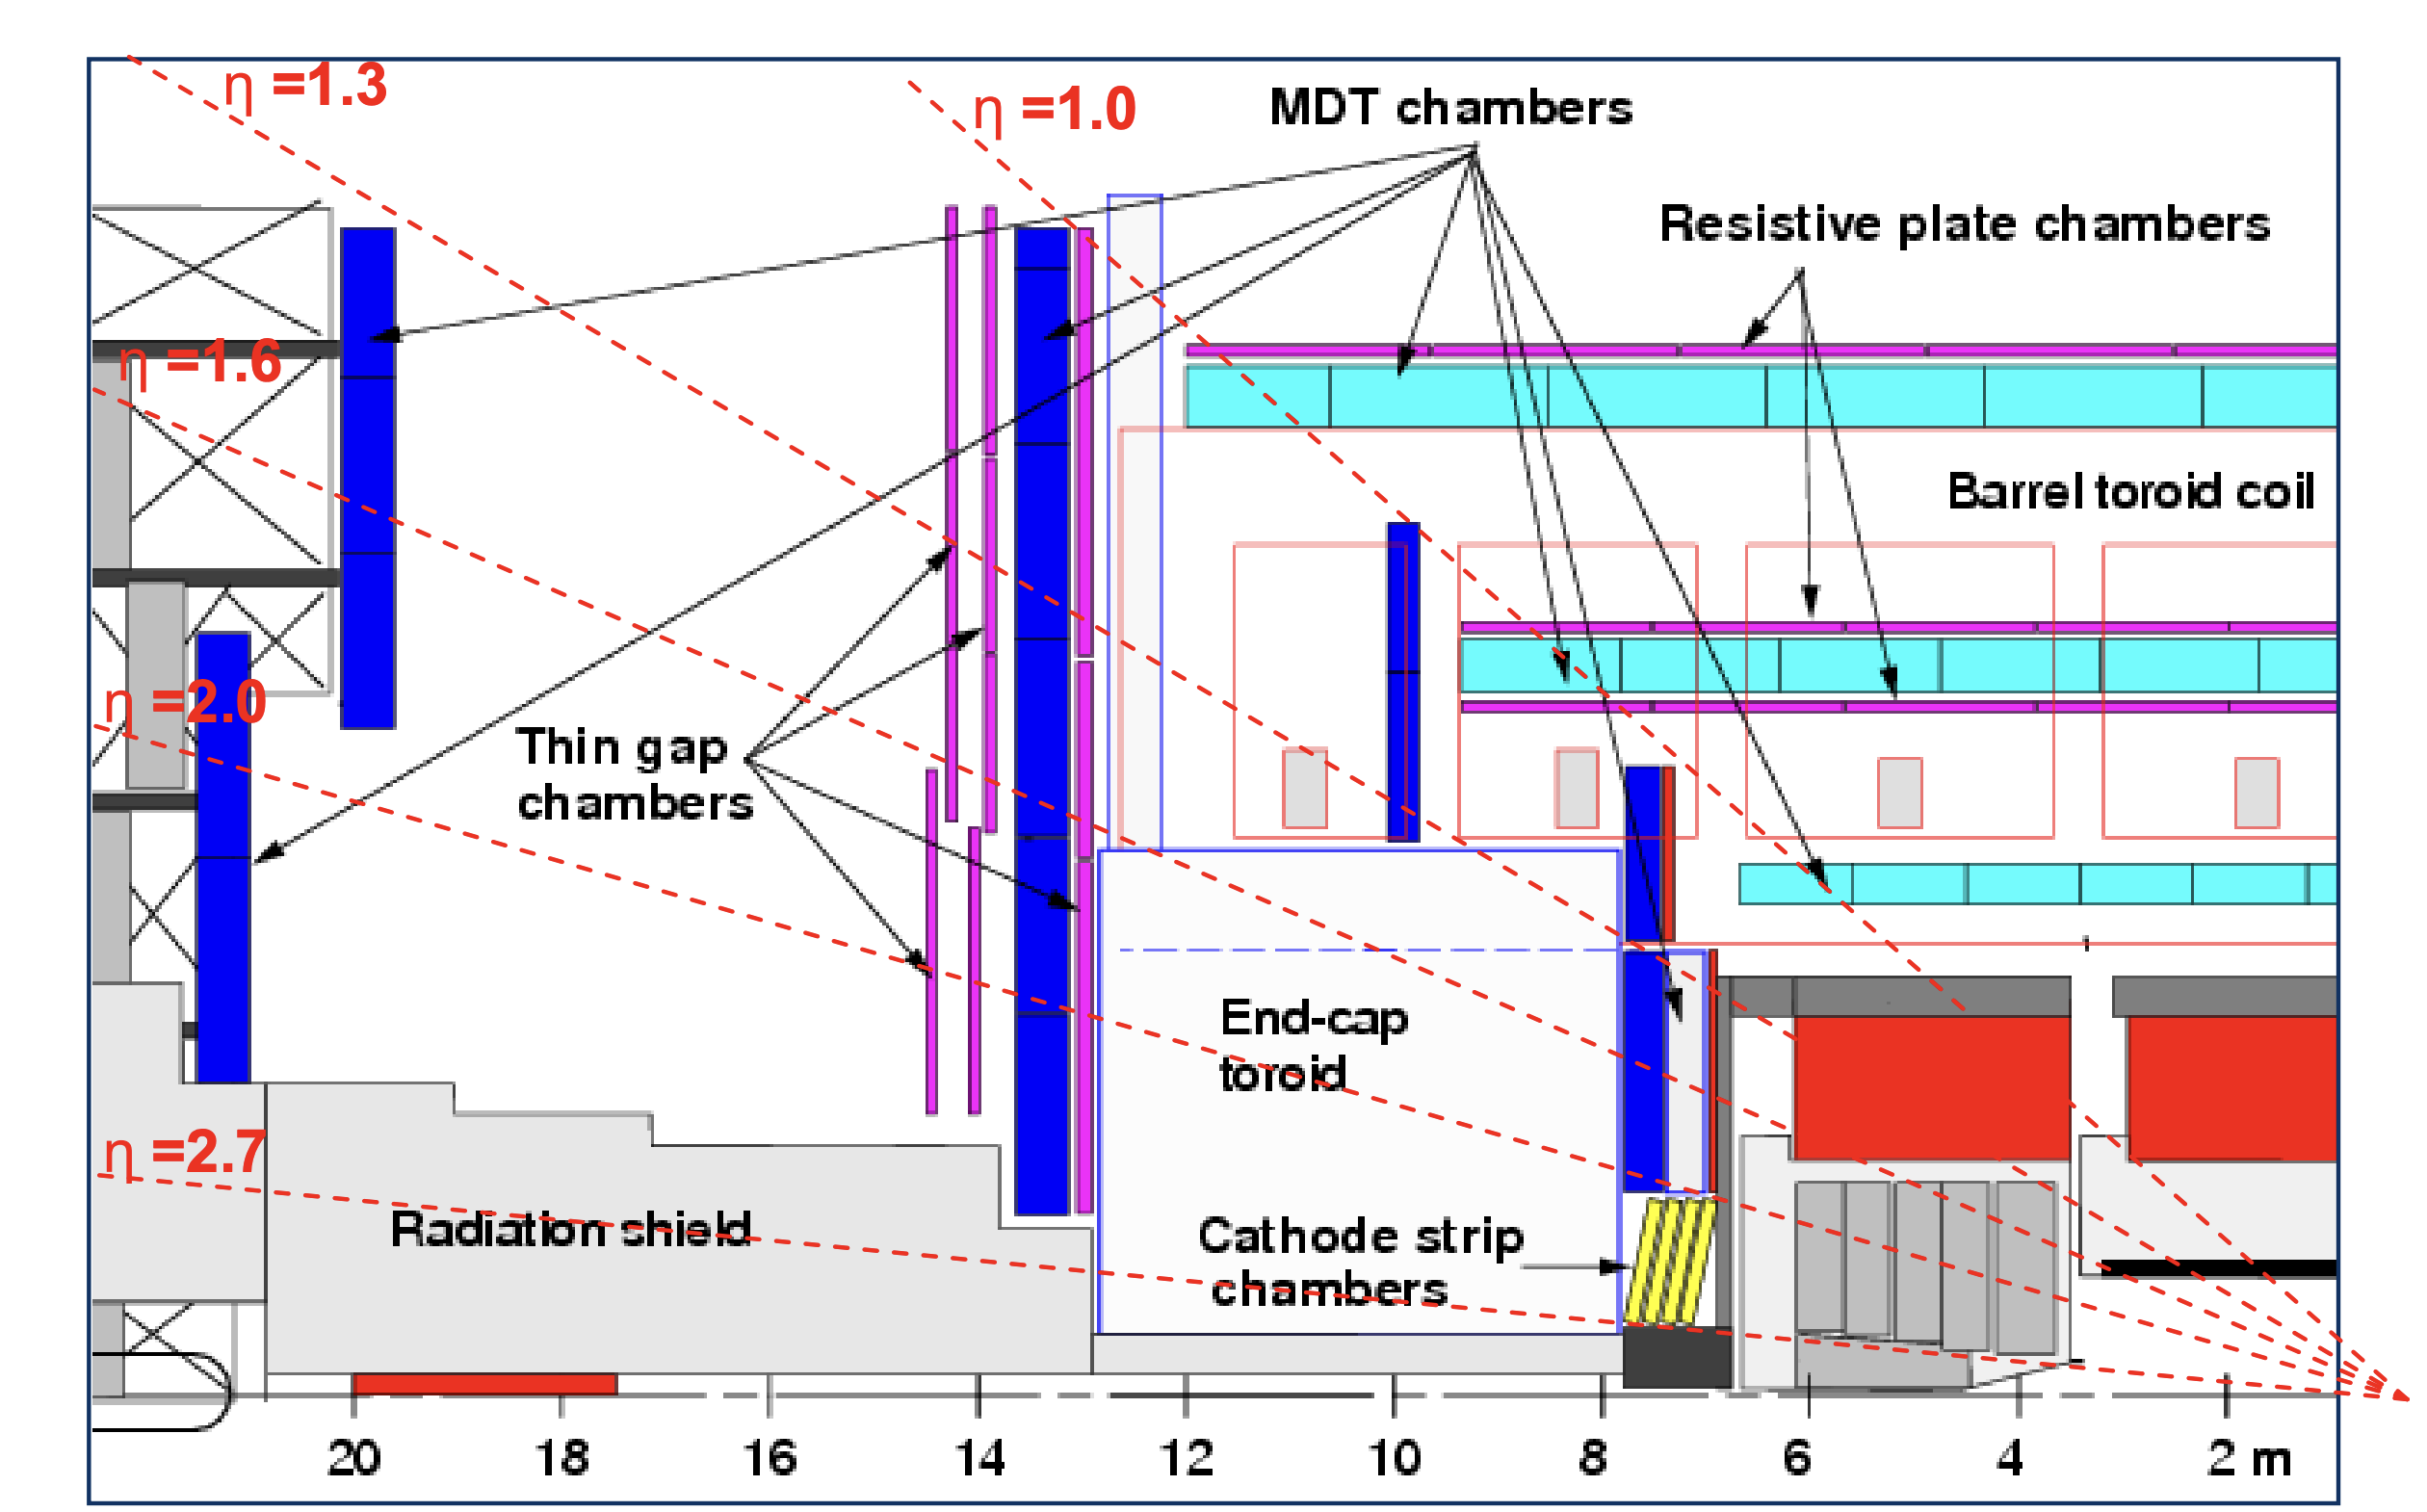
\includegraphics[width=.8\textwidth]{content/img/ATLAS qudrant labelled MS.png}
    \caption{One quadrant of the ATLAS detector. The components of the Muon Spectrometer are labelled \cite{Hough_Transform_CSC}}
    \label{fig:ATLAS_quadrant}
\end{figure}

\begin{figure}[h]
    \centering
    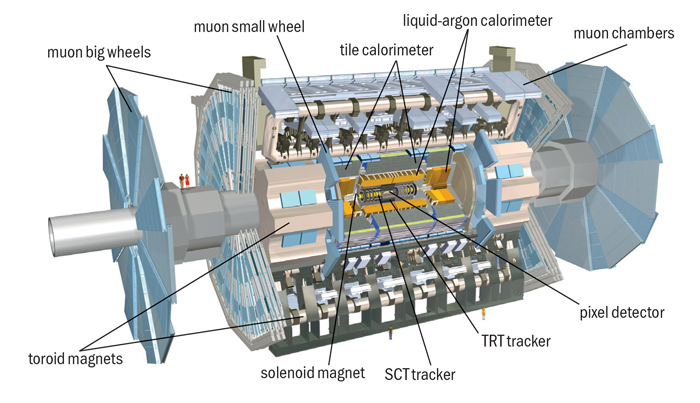
\includegraphics[width=.8\textwidth]{content/img/ATLAS_Detector.jpg}
    \caption{Overview of the ATLAS detectors main components, with two people in figure to scale.\cite{ATLAS_Illustration}}
    \label{fig:intro_ATLAS_detector}
\end{figure}

\noindent\textbf{Inner Detector}

The ATLAS detector is comprised of three main sections, the inner detector, calorimeters and the muon detector system. 
The inner detector measures the direction, momentum and charge of electrically charged particles.
Its main function is to measure the track of the charged particles without destroying the particle itself.
The first point of contact for particles emerging from $pp$-collisions from the center of the ATLAS detector is the pixel detector.\cite{PixelDetector_2008}
It has over 92 million pixels to aid in particle track and vertex reconstruction.
Since the pixels are the first point of contact to the incident particles they have to be radiation hard so the electronics may function without fault.
When a charged particle passes through a pixel sensor it ionizes the one-sided doped-silicon wafer to produce an excited electron will then occupy the conduction band of the semiconductor producing an electron-hole pair, leaving the valence band empty.\cite{KnollRadDetection}
This hole in the valence band together with the excited electron in the conduction band is called an electron-hole pair.
The electron-hole pair is in the presence of an electric field, which will induce drifting of the electron-hole pair, drifting that will generate the electric current to be measured.

Surrounding the pixel detector is the SemiConductor Tracker (SCT), which uses 4,088 modules of 6 million implanted silicon readout strips.\cite{ABDESSELAM2006642}
Both the pixel detector and SCT measure the path particles take, called tracks.
While the pixel detector has measurement precision up to $10 \mu m$ in the $r\phi$-direction and $70 \mu m$ in the $z$-coordinate direction,\cite{Andreazza:1287089} the SCT has resolution $17 \mu m$ in the $r\phi$-direction and $580 \mu m$ in the $z$-direction. 

The final layer of the inner detector is the transition radiation tracker (TRT). 
The TRT is made of a collection of tubes made with many layers of different materials with varying indices of refraction.
The TRT's straw walls are made of two $35\mu m$ layers comprised of $6\mu m$ carbon-polymide, $0.20 \mu m$ aluminum, and a $25\mu m$ Kapton film reflected back.\cite{TRT_2008}
The straws are filled with a gas mixture of $70\% \text{Xe} + 27\% \text{CO}_2 + 3\% \text{O}_2$. 
Its measurement precision is around $170 \mu m$. 
Particles with relativistic velocities have higher Lorentz $\gamma$-factors,
\begin{equation}\label{lorentzGamma}
    \gamma = \frac{1}{\sqrt{1 - \frac{v^2}{c^2}}}.
\end{equation}
The TRT uses varying materials to discriminate between heavier particles, which have low $\gamma$ and radiate less, and lighter particles, which have higher $\gamma$ and radiate more.\cite{Mindur:2139567}

\pagebreak
\noindent\textbf{Calorimeters}

There are two main calorimeters for ATLAS, the Liquid Argon (LAr) calorimeter and the Tile Hadronic calorimeter.
The LAr calorimeter surrounds the inner detector and measures the energy deposits of objects that interact via the electromagnetic force. 
It layers various metals to intercept the incoming particles to produce a shower of lower energy particles. 
The lower energy particles then ionize the liquid argon that fill the barrier in between the metal layers to produce a current that can be read out.
The Tile calorimeter surrounds the LAr calorimeter and is the largest part of the ATLAS detector weighing in around 2900 tons. 
Particles then traverse through the layers of steel and plastic scintillating tiles. 
The Tile calorimeter is a hadronic calorimeter, so it interacts with particles via the strong nuclear force. 
When a particle hits the steel, a cascade of secondary protons, neutrons and other hadrons (quark bound states, with baryons $qqq$ and mesons $q\bar{q}$) is produced with lower energy. 
Through this mechanism, these decay products will continue until the energy has entirely dissipated.

% Discuss the Muon spectrometer
\noindent\textbf{Muon Spectrometer (MS)}

The MS sits at the end of the ATLAS detector and is designed to identify muon tracks and momentum to high-resolution, its components are shown in Figure \ref{fig:ATLAS_quadrant}.
Monitored Drift Tube (MDT) chambers are used for precision measurement of muon tracks in the principle bending direction of the magnetic fields over a large $\eta$.
The MDT lie in the endcaps and barrel regions covering the pseudorapidity regions $0 < |\eta| < 2.7$, where the the tubes run perpendicular to the beam and in-line with the magnetic field lines.
Single cell resolution for these drift tubes can reach $60 \mu m$.\cite{ATLAS_Tech_Proposal}
The area of highest particle flux is the region of pseudo-rapidity $2 < |\eta| < 2.7$, here is where the cathode strip chambers lie.\cite{muonSpec}
Cathode strip chambers (CSCs) are layered to determine track vectors and use multi-wire chambers to achieve a resolution up to $50 \mu m$. 

The RPCs are gaseous parallel-plate detectors suited for fast spacetime particle tracking that combines the the spatial resolution (around 1 cm) of the wire chambers and the time resolution (around 1 ns) of a scintillation counter.
Resistive plate chambers (RPCs) and the Thin gap chambers (TGCs) provide the trigger information for the MDTs and CSCs to then make a precision measurement, so speed takes priority over spatial resolution for the muon trigger system. 
Though RPCs don't have wires, their design consists of two strips separated by an insulating spacer to create a gap for the gas ($C_2 H_2 F_4$ plus some smaller of argon/butane) to occupy.
Thin gap chambers (TGCs) exist in the forward region and are thin wire chambers that aide in muon triggering and measurement of the azimuthal coordinate to be used in compliment with MDTs.
The time resolution in TCGs help identify bunch-crossings and granularity in momentum of the muon that comes within the equipotential of the wires. 
Since each wire can be given a position in the trigger system, any muon that passes through the TGC can be compared with greater spatial precision with the MDTs and illustrate a track later.
The accuracy of identifying the correct bunch crossing with TGCs is 99\% and the delivery of bunch crossing identification can be delivered within 25 ns, only a small fraction of bunch crossings arrive later than that window.

\section{ATLAS Trigger/Data Acquisition (TDAQ)}

The LHC produces $pp$-collisions at a rate of 40 MHz, each collision is an ``event". 
More specifically, around $10^{11}$ protons are accelerated in one ``bunch" with around 2800 bunches per proton beam, spaced around 25 ns apart from each other. 
Each beam is then concentrated to the width of $64 \mu m$ at the interaction point where about 20 collisions happen at one bunch crossing. 
``Pile-up'' is the result of multiple collisions occurring from one bunch crossing.

% What is the ATLAS Trigger Systems
The ATLAS Trigger system is responsible for quickly deciding what events are interesting for physics analysis.
The Trigger system is divided into the first- and second-level triggers and when a particle activates a trigger, the trigger makes a decision to tell the DAQ to save the data produced by the detector. 
The first-level trigger is a hardware trigger that decides, within $2.5 \mu s$ after the event, if the event is good to put into a storage buffer for the second-level trigger.
The second-level trigger is a software trigger that decides within $200 \mu s$ and uses around 40,000 CPU-cores and analyses the event to decide if it is worth keeping. 
The second-level trigger selects about 1000 events per second to keep and store long-term.\cite{Trigger-DAQ}
The data taken by the TDAQ system is raw and not yet in a state that is ready for analysis, but it is ready for further processing. 

% Lots of data -> WLCG handles it
The amount of data taken at ATLAS is substantial, seeing more than 3 PB of raw data each year and each individual event being around 2 MB.\cite{ATLAS_Fact_Sheet} 
All of the data produced by LHC experiments, especially ATLAS, has to be sent to the Worldwide LHC Computing Grid (WLCG).\cite{WLCG_Tech_design_report}
% How is it sent to the Grid: Tier 0, 1, 2 sites
The WLCG composes of a three-tiered system, CERN serves as the Tier-0 site, there are $\mathcal{O}(20)$ Tier-1 sites, and $\mathcal{O}(200)$ Tier-2 sites.\cite{Martelli_2015}
Though, the numbers of each site do change over time.
The raw data coming from the TDAQ systems are recorded at the CERN Tier-0 sites where a first-pass at reconstruction will take place and a copy of the raw data is sent to the Tier-1 sites.
Multiple 10 Gbps capacity links streamline dataflow from the ATLAS TDAQ to the Tier-0 site. 
Tier-1 sites offer manage permanent storage of raw and reconstructed data and provide extensive processing capability for analysis that might demand it.
Tier-2 sites provide additional computation and storage services that compliment end-user analysis.

% WLCG handles it -> in what way is it being handled?
Athena manages ATLAS production workflows which are involved with simulation of data and event generation, track reconstruction from hits, and derivation production.\cite{athenadocs}
Figure \ref{fig:ATLAS_data_chain} illustrates the broadstrokes of the entire ATLAS data processing chain for both real detector data and Monte Carlo (MC) simulations. 
MC simulation starts with the event generation (EVNT), following simulation of events hitting the detector (HITS) and further simulation of what would be read out of the detector (RDO).
The reconstructed Analysis Object Data (AOD) are then processed through derivation production jobs that reduces AODs through several steps of skimming, thinning and slimming data and from $\mathcal{O}(1)$ MB per event to $\mathcal{O}(10)$ kB per event, creating Derived AOD (DAOD).
An AOD contains converted detector signals into physics objects such as particle tracks, electron and muon candidates, primary vertices, and more.\cite{Aad:2895022}
AODs are used to simulate pile-up, 
Further discussion on the production of DAOD can be found in Section \ref{section: ATLASIO_Derivation}.
\begin{figure}[ht]
    \centering
    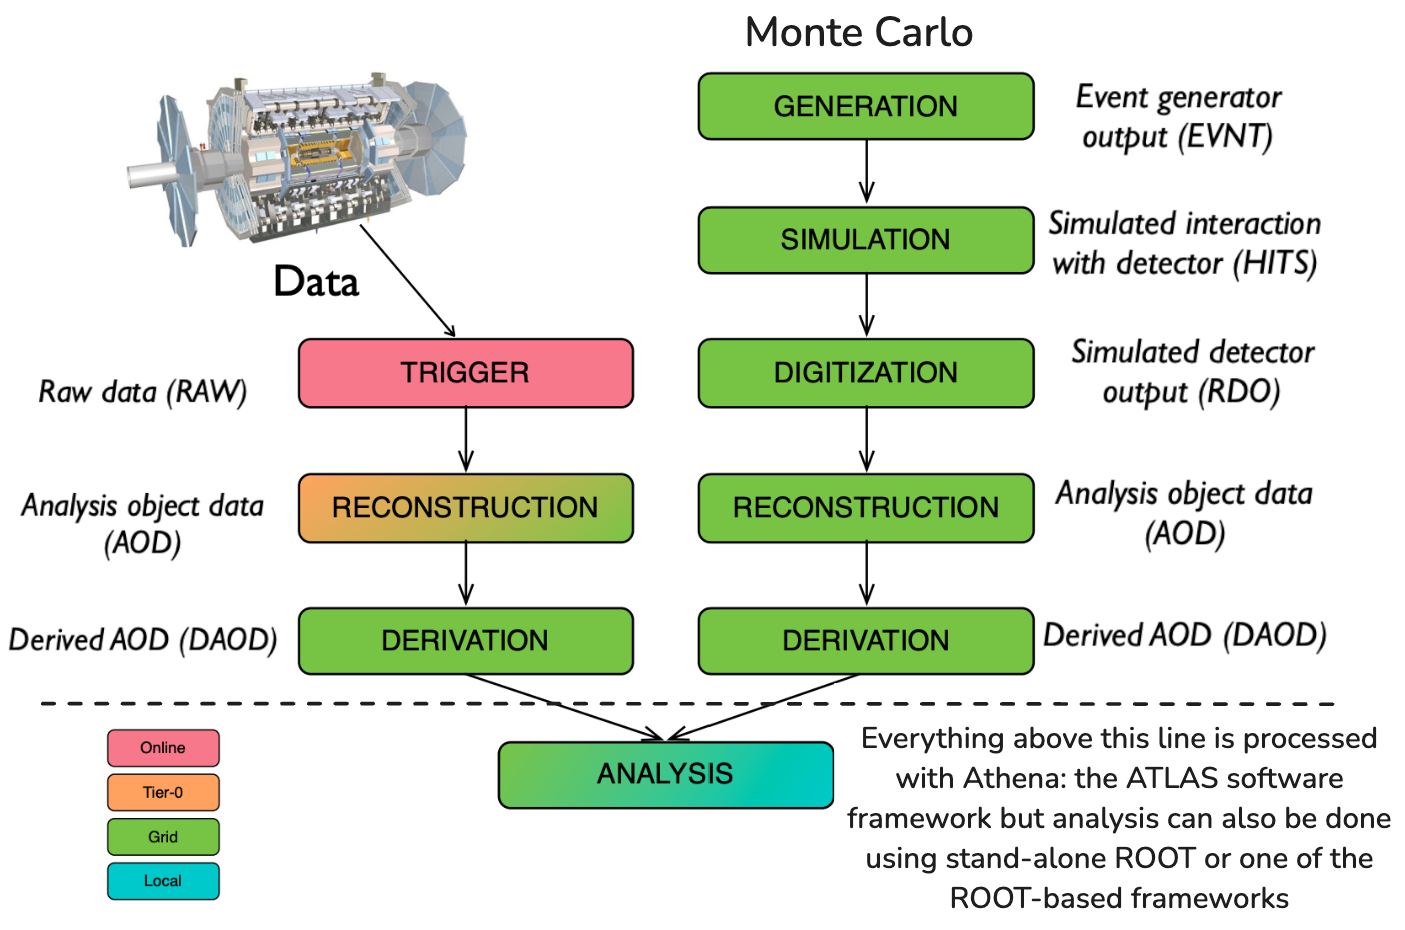
\includegraphics[width=\textwidth]{content/img/modified-James-chain-processing.png}
    \caption{ATLAS data chain-processing for data and Monte Carlo simulation. Figure is modified from \cite{James_Catmore_chain_processing}.}
    \label{fig:ATLAS_data_chain}
\end{figure}



\section{ATLAS Software and Computing Needs}
The High-Luminosity LHC (HL-LHC) is the upgrade to LHC that anticipates more events and more data taken than ever before.
% How does high luminosity affect the number of collisions? 
The goal is to reach a luminosity of $350 fb^{-1}$, which is forecasted to be reached gradually by around 2040.\cite{HL-LHC_Tech_design}
The HL-LHC era will start sooner than that, and has been projected to demand anywhere from 6-10 times data stored per year, so any attempt to save on disk storage should be investigated.\cite{ATLAS_HL-LHC_projections}
Increasing data means more resources from the Grid will be used, so optimization across files and software is an essential part of ensuring scalability of the data taken in by the detector.
Figure \ref{fig:intro_computing_models} illustrates the projections of the HL-LHC era long-term storage usage for both disk and tape. 

\begin{figure}[h]
    \centering
    \begin{subfigure}{.5\textwidth}
        \centering
        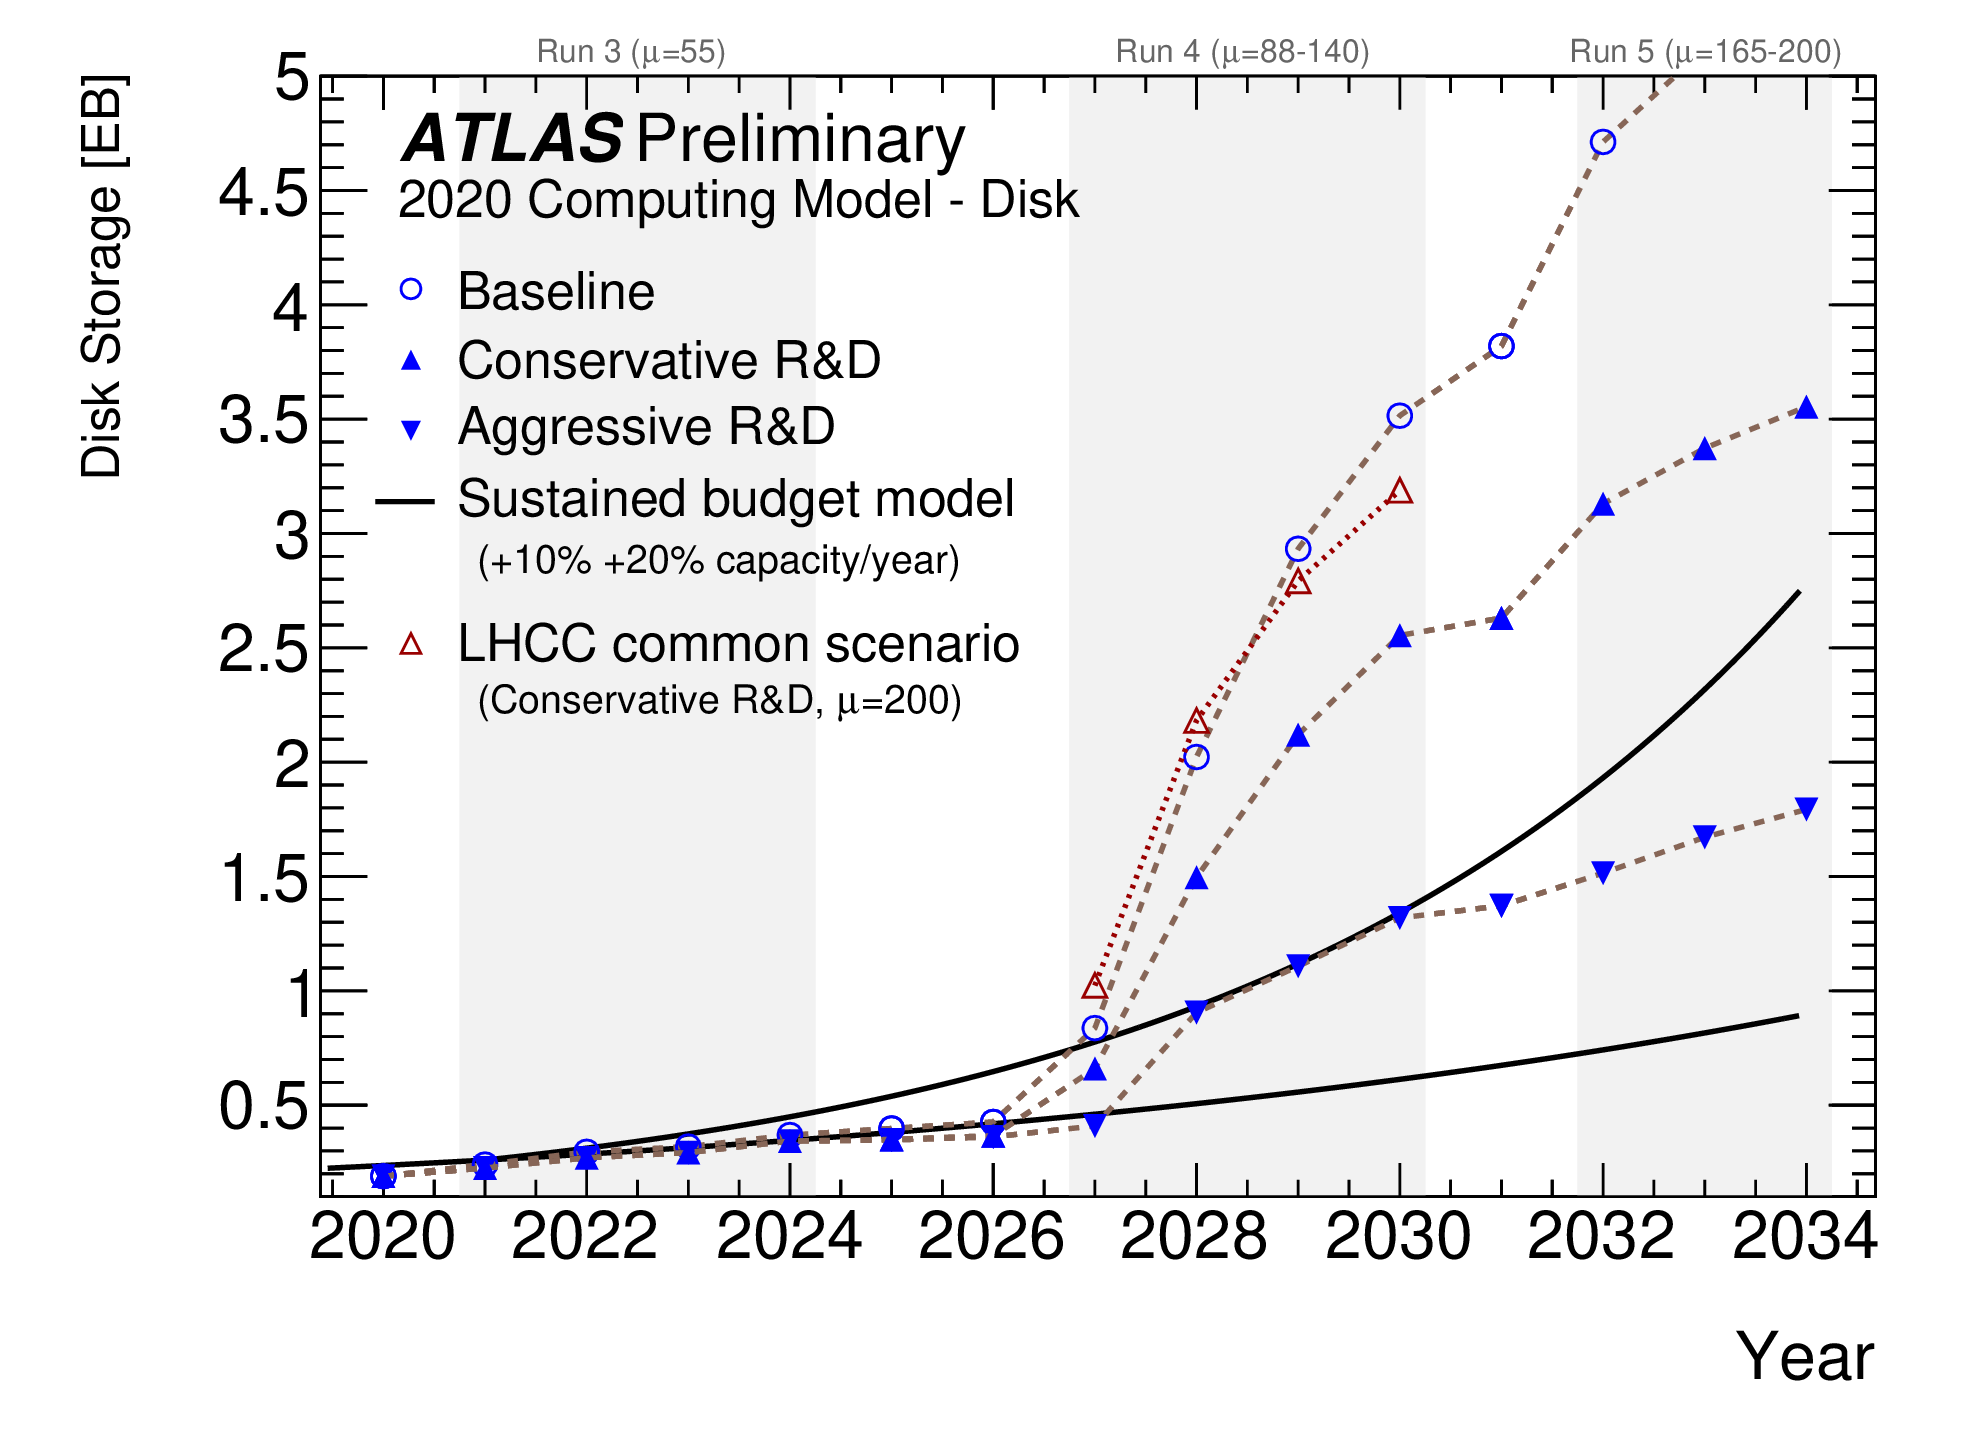
\includegraphics[width=\textwidth]{content/img/computing model-disk.png}
        % \caption{A subfigure}
        \label{fig:intro_computing_disk}
      \end{subfigure}%     
      \begin{subfigure}{.5\textwidth}
        \centering
        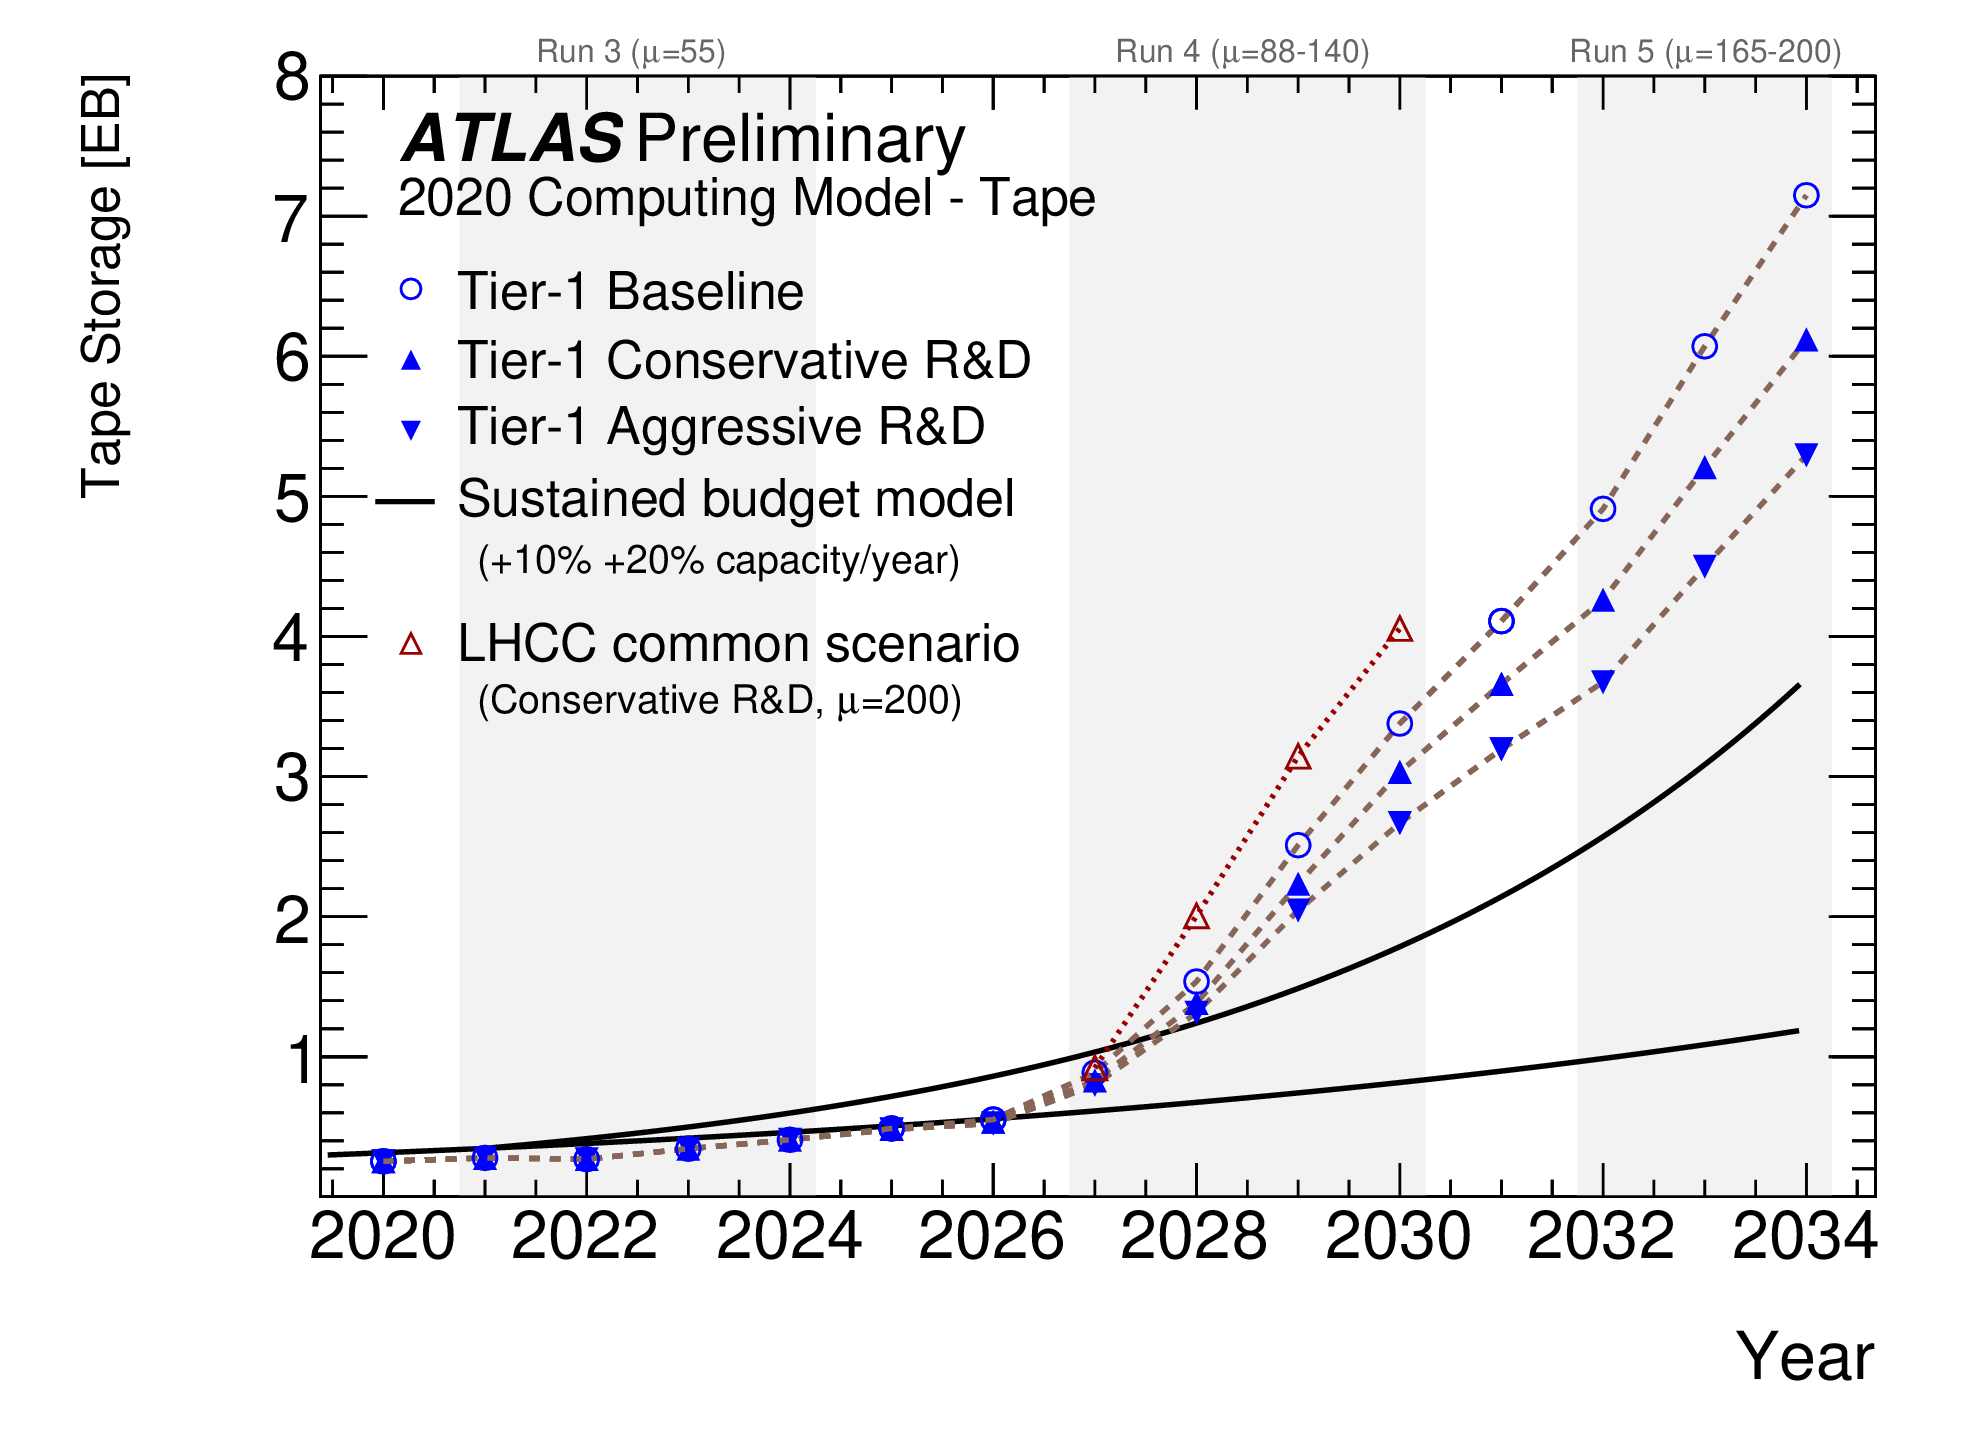
\includegraphics[width=\textwidth]{content/img/computing model-tape.png}
        % \caption{B subfigure}
        \label{fig:intro_computing_tape}
    \end{subfigure}% 
    \caption{HL-LHC computing model projections on the future disk and tape usage compared to the expected budget increases.\cite{CERN-LHCC-2020-015}}
    \label{fig:intro_computing_models}
\end{figure}

% We've been using ROOT TTree for decades 
% in particular TTree is used to store event data 
One avenue optimization is being investigated is in the method of storing data to file.
The traditional method of storing event information for AOD/DAOD is with ROOT TTrees.
ROOT TTrees (referred to as ``TTrees" or ``trees") have been the standard data storage format for over two decades, and they provide a clear means of organizing and accessing physics objects for processing and analysis.
The development of the ROOT N-Tuple (RNTuple) I/O subsystem updates areas to support multi-thread processing, asynchronous I/O, object stores, and more.
It's been shown to outperform the TTree I/O subsystem and other storage formats in file size (by about 15\%), throughput, and compression, but still has more development before full implementation into the analysis pipeline.\cite{RNTuple_Lopez-Gomez_2023}\cite{RNTuple_Blomer}
While RNTuple is in development, there are still insights regarding resource usage optimization that are found by using TTree in its current state. 



% 2. ATLAS I/O 
% -- 
\chapter{I/O Tools}
\label{chap:IO_Tools}
% CHAPTER START
The Trigger/DAQ system sends and saves data from the detector to a persistent data storage solution.
The data at this stage needs to be reconstructed and consolidated into physics objects, or Analysis Object Data (AOD) files.
Creating AODs from data requires significant computation power and is undertaken by a software framework maintained by ATLAS called Athena.
This chapter will cover important tools and concepts used by ATLAS to run derivation jobs, as well as introduce data structures that represent event information. 

\section{Event Data Models} \label{sec:IO_EDM}
% \subsection{What is an Event Data Model}
An Event Data Model (EDM) is a collection of classes and their relationships to each other that provide a representation of an event detected with the goal of making it easier to use and manipulate by developers.
An EDM is how particles and jets are represented in memory, stored to disk, and manipulated in analysis.
It's useful to have an EDM because it brings a commonality to the code, aiding developers who reside in different groups often with various background experience.
An EDM allows those developers to more easily debug and communicate issues when they arise.  

\subsection{Transient/Persistent (T/P) EDM}
ATLAS used an EDM schema for Run-1 which had a separate transient and persistent status of the AODs.
AODs would often be converted to an ``ntuple" based format that allowed for fast readability and partial read for efficient analysis in ROOT, though it left the files disconnected from the reconstruction tools found in Athena.\cite{Athena_xAOD_design}
When transient data was present in memory, it could have information attached to the object and gain complexity the more it was used.
Transient data needed to be simplified before it could become persistent into long-term storage (sent to disk). 
ROOT had trouble handling the complex inheritance models that would come up the more developers used this EDM. 
Before the successor to the T/P EDM was created, ATLAS physicists would convert data samples using the full EDM to a simpler one that would be directly readable by ROOT.
This would lead to duplication of data and made it challenging to develop and maintain the analysis tools to be used on both the full EDM and the reduced ones.
Additionally, converting from transient to persistent data was an excessive step which was eventually no longer needed with the creation of an EDM that blends the two stages of data together, this is the xAOD EDM.

\subsection{xAOD EDM}
While the T/P EDM still remains functional in Athena, the xAOD EDM has been adopted as of Run 2. 
The xAOD EDM is an iteration to the T/P EDM and brings a variety of improvements.\cite{Buckley_2015}
This EDM, unlike T/P, is not strictly separated into transient or persistent data.
Rather, xAOD primarily separates data into interface objects and its corresponding auxiliary data stores.
The xAOD EDM has built-in functionality to add and remove dynamic attributes configured during job steering.
These dynamic attributes to xAOD objects are called decorations.

The xAOD EDM use two types of objects to handle data, interface and payload. 
Interfaces act as an access point for the user to call an object but without its stored data subsequently occupying space in memory. 
This differs from T/P where the user wants to load an object into memory to access the object. 
If the user wanted to read the data, they could use the interface object to do so, protecting the user from changes to the payload in the process. 
The payload object contains the data for the interface object and allocates contiguous blocks of memory. 
Payload classes are often referred to as auxiliary storage. 

The specific data structure used by ATLAS is the ROOT TTree, but the EDM is agnostic to the type of data structure used. 
ATLAS specific libraries are not required to handle files written in the xAOD format since the payload can be read directly from the contiguous allocation of memory, a central tenent of the xAOD EDM.
This allows for the separation of ATLAS specific analysis frameworks and the preferred analysis tool of the user.
More information on how the xAOD EDM is deployed into unit tests in Section \ref{sec:Mod_utests_xAOD_object}.

\section{Athena and ROOT}
% \subsection{What is Athena}
Athena is the open-source software framework for the ATLAS experiment.\cite{athena}
It is based off the Gaudi project and uses ROOT and other software from the LHC Computing Grid (LCG) software stack.\cite{WLCG_Tech_design_report}
The LCG software stack is a set of software frameworks that provide general solutions for the LHC experiment's computing needs. 
It contains on the order of 500 packages, which include binary builders and compilers, language libraries and dependencies, simulation and analysis software, and more.
Athena also provides some in-house based analysis tools as well as tools for specifically ROOT based analysis.

An Athena application relies on $\textit{components}$: Algorithms, Tools, Services and Properties. \cite{Aad:2895022}  
Each component plays a role in executing an Athena application or job, where $\textsc{Python}$ is used for job configuration and steering.\footnote{Job transforms are $\textsc{Python}$ scripts that steer Athena production jobs by configuring arguments that would alter low-level behavior of the entire job. }
Specifically, an Algorithm accesses data objects in the event store, as shown with the solid lines in Figure \ref{fig:ATLAS_Athena_Job_flow}, but does not own or provide any data itself.
Algorithms can ``own" Tools, which serve as helpers exclusive to Algorithms or other components that call them.\footnote{``Ownership" here refers to the components' exclusive access or control of a Tool or Service.} 
Services are not as exclusive with its access, as they can be used by other components to provide a service such as Athena-ROOT conversion, random number generators, and others. 
Properties are able to be called at initialization of the job configuration and include flag definitions, input and output file names, and other algorithm specific options.

\begin{figure}[ht]
  \centering
  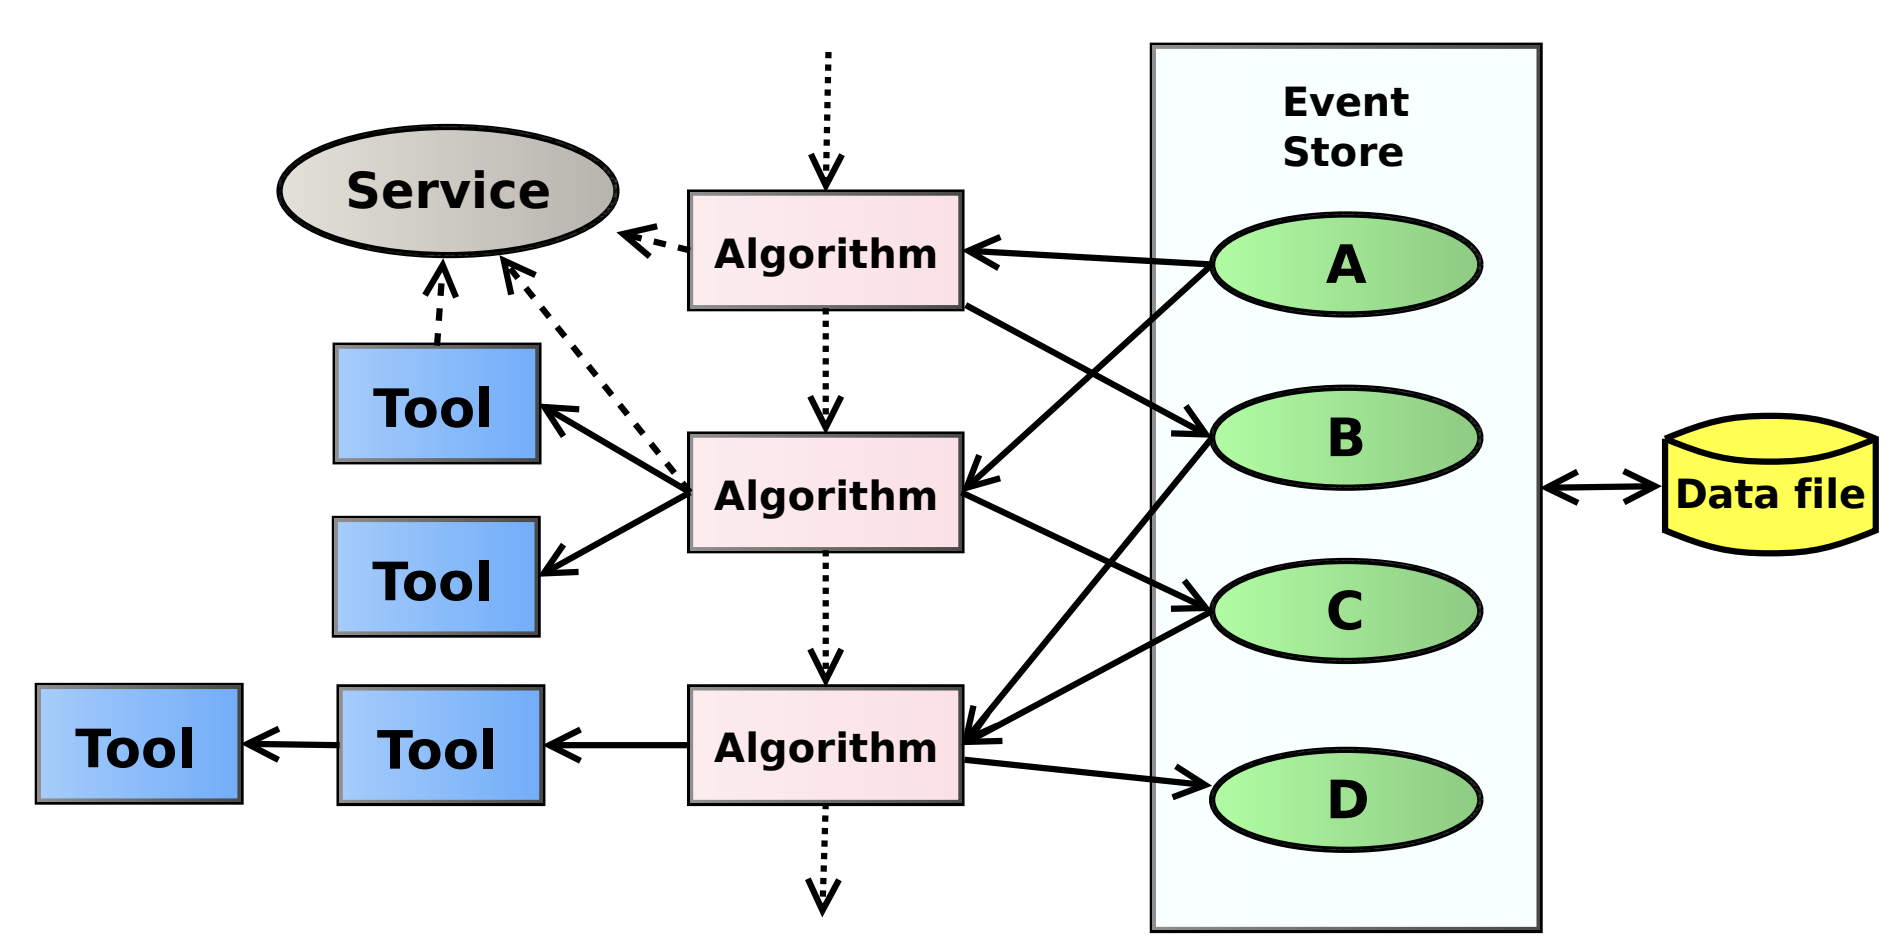
\includegraphics[width=0.8\textwidth]{content/img/athena job.png}
  \caption{An Athena application's general structure.\cite{Aad:2895022}}
  \label{fig:ATLAS_Athena_Job_flow}
\end{figure}

\verb|ComponentAccumulator| (CA) is a python class that put into Athena production as a way to prevent extra calls of setting flags during configuration. 
An important step throughout the development of Athena is to ensure any new changes to the codebase will not overrule the functionality of core features to the present workflows.
One of the areas needed to be tested before and upon merging of any new changes to Athena is the I/O functionality, or the performance of reading and writing of stored objects within a broader context of various jobs, i.e. reconstruction or derivation.
While CA is a more general mechanism to run many kinds of job with Athena, the scope of this thesis is using CA to test core I/O functionality of the new event data model. 
An example Athena job configuration is found in Appendix \ref{app:athena-job-config}. 

ROOT is an open-source software framework used for high-energy physics analysis at CERN.\cite{ROOT_about} 
It uses C++ objects to save, access, and process data brought in by the various experiments based at the LHC, the ATLAS experiment uses it in conjunction with Athena.
ROOT largely revolves around organization and manipulation of TFiles and TTrees into ROOT files.
A TTree represents a columnar dataset, and the list of columns are called branches. 
A TTree is a ROOT object that organizes physically distinct types of event data into TBranches, or just branches.
Event data could range from information about a specific type of interaction, this includes tracks, position of particles at one point in the detector. 

\begin{figure}[ht]
  \centering
  \vspace{20px}
  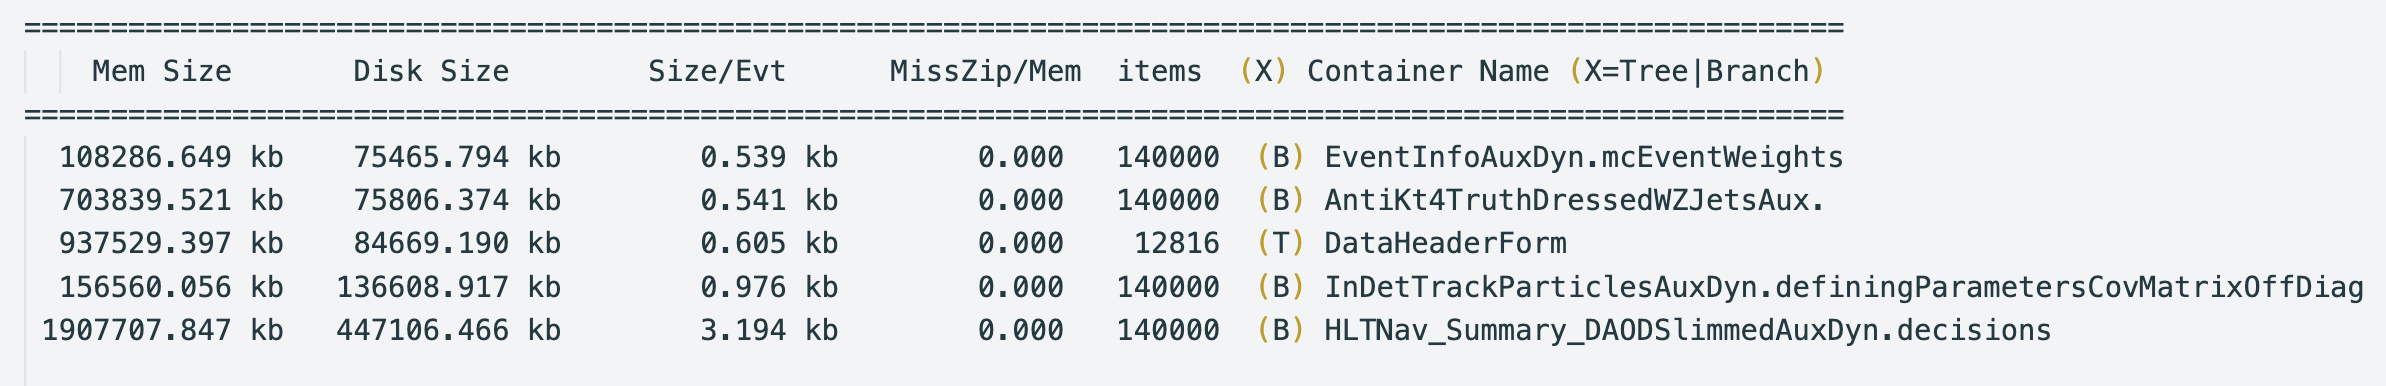
\includegraphics[width=\textwidth]{content/img/branches_in_TTree.png}
  \caption{A snapshot of the TBranches composing a TTree, from a PHYSLITE DAOD}
  \vspace{20px}
  \label{fig:Branches_in_TTree}
\end{figure}

One function relevant to TTree is \verb|Fill()|. 
\verb|Fill()| will loop over all of the branches in the TTree and compresses the baskets that make up the branch.\cite{ROOT_TTree}
This initiates the data in memory to start filling a branch's basket buffer (or just ``baskets").
While this first buffer is always unoptimized, it allows opportunity to calculate an optimal basket buffer size.
At regular intervals, dictated either by number of bytes written or by number of entries written, \verb|AutoFlush| will compress the buffers, store them into baskets, and move them from memory to disk. 
It's this ``flushing" mechanism that allows for easy access to the branch data as each of the baskets will be stored contiguously in memory.

The Athena default maximum basket size at present is 128 kB, and the default minimum number of entries is 10.
The minimum number of entries helps reduce processing on every entry which might be empty, and the maximum basket size is in place to prevent baskets from using too much memory throughout a Grid job.  
Prior to this thesis, the original implementation of both the basket size and minimum number of entries had not yet been fully investigated for avenues of optimization, this is explored in Section \ref{sec:DAODProd_Analysis}.

% % CMake
CMake and Make are open-source software that is used to build Athena, ROOT, and other software.
A sparse build is a way to make changes to an individual package of code without having to recompile the entire framework at once, which saves time and resources. 
A user can create a text file identifying the path to the package modified, and the sparse build for Athena will proceed upon issuing the following commands:
\begin{lstlisting}[language=bash]
    cmake -DATLAS_PACKAGE_FILTER_FILE=../package_filters.txt ../athena/Projects/WorkDir/ 
    make -j
\end{lstlisting}

% How we used it
% % Athena POOL
The POOL framework is part of a larger framework known as the Persistency Framework (PF). \cite{Trentadue_2012}
The PF was developed with the intent to be independent of any individual experiment, and the goal was to address data access requirements of LHC experiments in different ways.
POOL was in charge of C++ object storage, collection of metadata, and file catalogs by using streaming and relational technologies. 
POOL provided highly scalable object serialization to framework evolving PF files. 
It was eventually discontinued by other experiments in favor of a newer persistency mechanism that uses ROOT in a more streamlined way.
ATLAS then became the sole supporter of POOL and integrated it within Athena to support persistent navigation of the ROOT storage layer.
Now, Athena has both the original PF POOL functionality and a separate modern AthenaPool functionality. 
AthenaPool resides in the ATLAS I/O framework and controls ROOT TTree and TBranch properties such as compression and basket buffer sizing.
Within the subset of AthenaPool packages resides unit tests which will be expanded upon in Chapter \ref{chap:Modernize}.

% What we looked at/How we used it

\subsection{Continuous Integration (CI) and Development}
CI is a software development practice where new code is tested and validated upon each merge to the main branch of a repository. 
Every commit to the main branch is automatically built and tested for specific core features that are required to work with the codebase. 
This helps to ensure that the codebase is working as intended and that any new code is compatible with the existing codebase.

Athena is hosted on GitLab and developed using CI with an instance of Jenkins, called ATLAS Robot, which builds and tests the new changes within a merge request interface.\cite{athena-gitlab}\cite{Jenkins}
ATLAS Robot will then provide a report of the build and test results.
If the build or test fail, ATLAS Robot will provide a report of which steps failed and why.
This allows for early detection of issues before the nightly build is compiled and tested.


\section{Derivation Production Jobs}
 \label{section: ATLASIO_Derivation}

A derivation production job takes AODs, which comes from the reconstruction step at $\mathcal{O}(1 \text{ MB})$ per event, and creates a derived AOD (DAOD) which sits at $\mathcal{O}(10 \text{ kB})$ per event.
Derivation production is a necessary step to make all data accessible for physicists doing analysis as well as reducing the amount of data that needs to be processed.
While derivations are reduced AODs, they often contain additional information useful for analysis, such as jet collections and high-level discriminants.\cite{PHYSLITE_A_new_2024}
The two mainstream output file formats Athena is capable of handling are PHYS and PHYSLITE.  
Derivation production jobs for both PHYS and PHYSLITE can demand heavy resource usage on the GRID, so optimization of the AOD/DAODs for these jobs are vital. 

% TODO: How does MC differ from Data in terms of composition? 

Figure \ref{fig:IO_tt_PHYS_vs_PHYSLITE} shows the object composition of a PHYS and PHYSLITE $t\bar{t}$ simulated sample. 
In this instance, PHYS output files, at 40.0 kB per event, are predominantly made of jet collections, while PHYSLITE files, at 16.1 kB per event, have more trigger-related and track information.
The composition of DAODs, both PHYS and PHYSLITE, produced by derivation jobs may change over time, but the overall size per event for each format is sought to remain the same. 

\begin{figure}[h]
  \centering
  \vspace{20px}
  \begin{subfigure}{.5\textwidth}
      \centering
      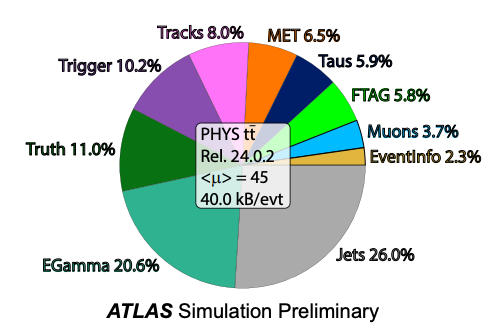
\includegraphics[width=\textwidth]{content/img/tt_PHYS.png}
      % \caption{A subfigure}
      \label{fig:IO_tt_PHYS_subA}
    \end{subfigure}%     
    \begin{subfigure}{.5\textwidth}
      \centering
      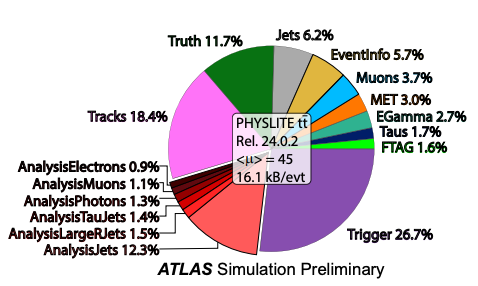
\includegraphics[width=\textwidth]{content/img/tt_PHYSLITE.png}
      % \caption{B subfigure}
      \label{fig:IO_tt_PHYSLITE_subB}
    \end{subfigure}% 
  \caption{Object composition of a PHYS and PHYSLITE $t\bar{t}$ MC simulated sample from Run 3.}
  \vspace{10px}
  \label{fig:IO_tt_PHYS_vs_PHYSLITE}
\end{figure}


The derivation framework, seen in Figure \ref{fig:IO_derivation_framework}, is sequence of steps that are performed on the AODs to create the DAODs.
Skimming is the first step in the derivation framework, and is responsible for removing whole events based on pre-defined (or augmented) criteria.
Thinning is the second step, and it removes whole objects based on similarly pre-defined or augmentable criteria.
Lastly slimming removes variables from objects uniformly across events. 


\begin{figure}[h]
  \centering
  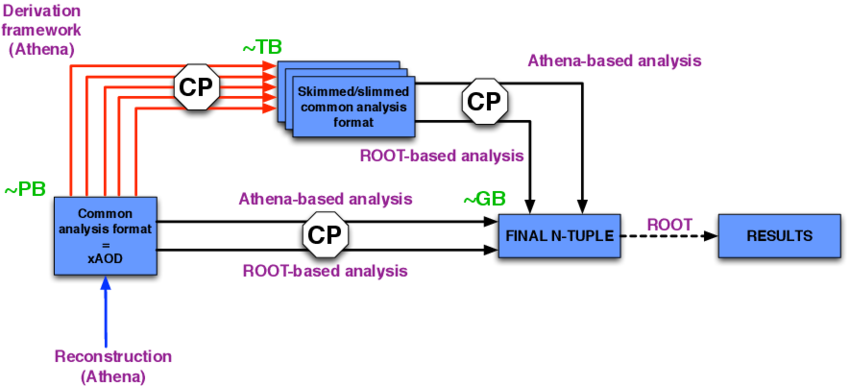
\includegraphics[width=0.8\textwidth]{content/img/catmore-derivation.png}
  \caption{Derivation production from Reconstruction to Final N-Tuple\cite{DAOD_Laycock_2014}}
  \label{fig:IO_derivation_framework}
\end{figure}

% 3. Toy Model Branches
% -- 
\chapter{Toy Model Branch Study}
\label{chap:Toy_Model}
Building a toy model for derivation production jobs offers a simplified framework to effectively simulate and analyze the behavior of real and Monte Carlo (MC) data.
A toy model collection of data can mimic commonalities in both data and MC by filling in branches with a mixture of position coordinate information, momenta, or other details about the detector.  

Integers that are repeated can be easier to compress than floating-point numbers of increased precision, so adjusting the ratio of integers to floats creates a mixture which can yield compression ratios closer to real experimental and MC simulated data.  
Replicating this mixture in a branch give us an effective model that resembles how basket buffer optimization might affect the compression of real and MC simulated data. 
In other words, these toy model mixtures provide an avenue to test opportunities for optimizing the memory and storage demands of the GRID by first looking at limiting basket sizes and their effects on the compression of branches. 

\section{Toy Model Compression}

\subsection{Random Float Branches} \label{sec:toy_compression_random_float_branches}
There were a number of iterations to the toy model, but the first was constructed by filling a TTree with branches that each have vectors with varying number of random floats to write and read.
Vectors are used in this toy model, as opposed to arrays, because vectors are dynamically allocated and deallocated, which allows for more flexibility when synthesizing AODs. 
This original model had four distinct branches, each with a set number of events (\verb|N=1000|), and each event haivng a branch with a vector. 
Depending on the kind of branch, a vector would have either 1, 10, 100, or 1000 floating point vector-entries.
The script can be compiled with \verb|gcc| or \verb|g++| and it requires all of the dependencies that come with ROOT. 
Alternatively, the script can be run directly within ROOT.

The following function \verb|VectorTree()| is the main function in this code.
What is needed first is an output file, which will be called \verb|VectorTreeFile.root|, and the name of the tree can simply be \verb|myTree|.
% \begin{lstlisting}[language=C]
%   void VectorTree() {
%     std::unique_ptr<TFile> myFile =
%     std::make_unique<TFile>("VectorTreeFile.root", "RECREATE");
%     TTree *tree = new TTree("myTree", "myTree");
%     ...
%   }
% \end{lstlisting}
The toy model starts variable initialization with the total number of events in the branch, i.e. the number of times a branch is filled with the specified numbers per vectors, \verb|N|. 
Additionally the branches have a number of floats per vector, this size will need to be defined as \verb|size_vec_0|, \verb|size_vec_1|, etc.  
The actual vectors that are being stored into each branch need to be defined as well as the temporary placeholder variable for our randomized floats, \verb|vec_tenX| and \verb|float_X|, respectively. 
\begin{lstlisting}[language=C]  
  void VectorTree() {
    ...
    const int N = 1e4; // N = 10000, number of events
    // Set size of vectors with 10^# of random floats
    int size_vec_0 = 1;
    int size_vec_1 = 10;
    int size_vec_2 = 100;
    int size_vec_3 = 1000;

    // vectors
    std::vector<float> vec_ten0; // 10^0 = 1 entry
    std::vector<float> vec_ten1; // 10^1 = 10 entries
    std::vector<float> vec_ten2; // 10^2 = 100 entries
    std::vector<float> vec_ten3; // 10^3 = 1000 entries

    // variables
    float float_0;
    float float_1;
    float float_2;
    float float_3;
    ...
  }
\end{lstlisting}

From here, branches are initialized so each one knows where its vector pair resides in memory.
\begin{lstlisting}[language=C]  
  void VectorTree() {
    ...
    // Initializing branches
    std::cout << "creating branches" << std::endl;
    tree->Branch("branch_of_vectors_size_one", &vec_ten0);
    tree->Branch("branch_of_vectors_size_ten", &vec_ten1);
    tree->Branch("branch_of_vectors_size_hundred", &vec_ten2);
    tree->Branch("branch_of_vectors_size_thousand", &vec_ten3);
    ...
  }
\end{lstlisting}

One extra step taken during this phase of testing is the disabling of \verb|AutoFlush|. 
\begin{lstlisting}
  void VectorTree() {
    ...
    tree->SetAutoFlush(0);
    ...
\end{lstlisting}
Disabling \verb|AutoFlush| allows for more consistent compression across the various sizes of branch baskets. 
If \verb|AutoFlush| were enabled, then across the various branch types, as in \ref{fig:toymodel_compF_rndm_vectors}, ROOT would decide when to compress each branch basket preventing a consistent compression configuration for the toy model.  
The derivation production jobs tested in Chapter $\ref{chap:DAODProd}$ were tested with \verb|AutoFlush| enabled because those tests are focused on memory and disk usage as opposed to mimicking real or MC data, which they are already using.
Following branch initialization comes the event loop where data is generated and emplaced into vectors.

\begin{lstlisting}[language=C]  
  void VectorTree() {
    ...
    // Events Loop
    std::cout << "generating events..." << std::endl;
    for (int j = 0; j < N; j++) {
        // Clearing entries from previous iteration
        vec_ten0.clear();
        vec_ten1.clear();
        vec_ten2.clear();
        vec_ten3.clear();

        // Generating vector elements, filling vectors
        // Fill vec_ten0 
        // Contents of the vector:
        //    {float_0}
        //    Only one float of random value
        float_0 = gRandom->Rndm() * 10; // Create random float value
        vec_ten0.emplace_back(float_0); // Emplace float into vector
        
        // Fill vec_ten1
        // Contents of the vector:
        //    {float_1_0, ... , float_1_10}
        //    Ten floats, each float is random
        for (int n = 0, n < size_vec_1; n++) {
            float_1 = gRandom->Rndm() * 10;
            vec_ten1.emplace_back(float_1);
        }

        // Do the same with vec_ten2 and vec_ten3, except for 
        //     vectors with size 100 and 1000 respectively. 
        
        // After all branches are filled, fill the TTree with 
        //     new branches
        tree->Fill();
    }
    // Saving tree and file
    tree->Write();
    ...
  }
\end{lstlisting}
Once the branches were filled, ROOT then will loop over each of the branches in the TTree and at regular intervals will remove the baskets from memory, compress, and write the baskets to disk (flushed).

As illustrated, the \verb|TTree| is written to the file which allows for the last steps within this script. 

\begin{lstlisting}[language=C]  
  void VectorTree() {
    ...
    // Look in the tree
    tree->Scan();
    tree->Print();

    myFile->Save();
    myFile->Close();
  }
  int main() {
    VectorTree();
    return 0;
  } 
\end{lstlisting}

Upon reading back the ROOT file, the user can view the original size of the file (Total-file-size), the compressed file size (File-size), the ratio between Total-file-size and File-size (Compression Factor), the number of baskets per branch, the basket size, and other information. 
Filling vectors with entirely random values was believed to yield compression ratios close to real data, but the results in Figure \ref{fig:toymodel_compF_rndm_vectors} show changes needed to be made to bring the branches closer to a compression ratio of $\mathcal{O}(5)$.\footnote{This compression factor comes as the average branch compression factor post-derivation job, which is discussed in Section \ref{section: ATLASIO_Derivation}} 
It is evident that branches containing vectors with purely random floats are more difficult to compress due to the high level of randomization.
Figure \ref{fig:toymodel_compF_rndm_vectors} shows compression drop-off as the branches with more randomized floats per vector were present.
This is the leading indication that there needs to be more compressible data within the branches. 
\vspace{20px}
\begin{figure}[h]
    \centering
    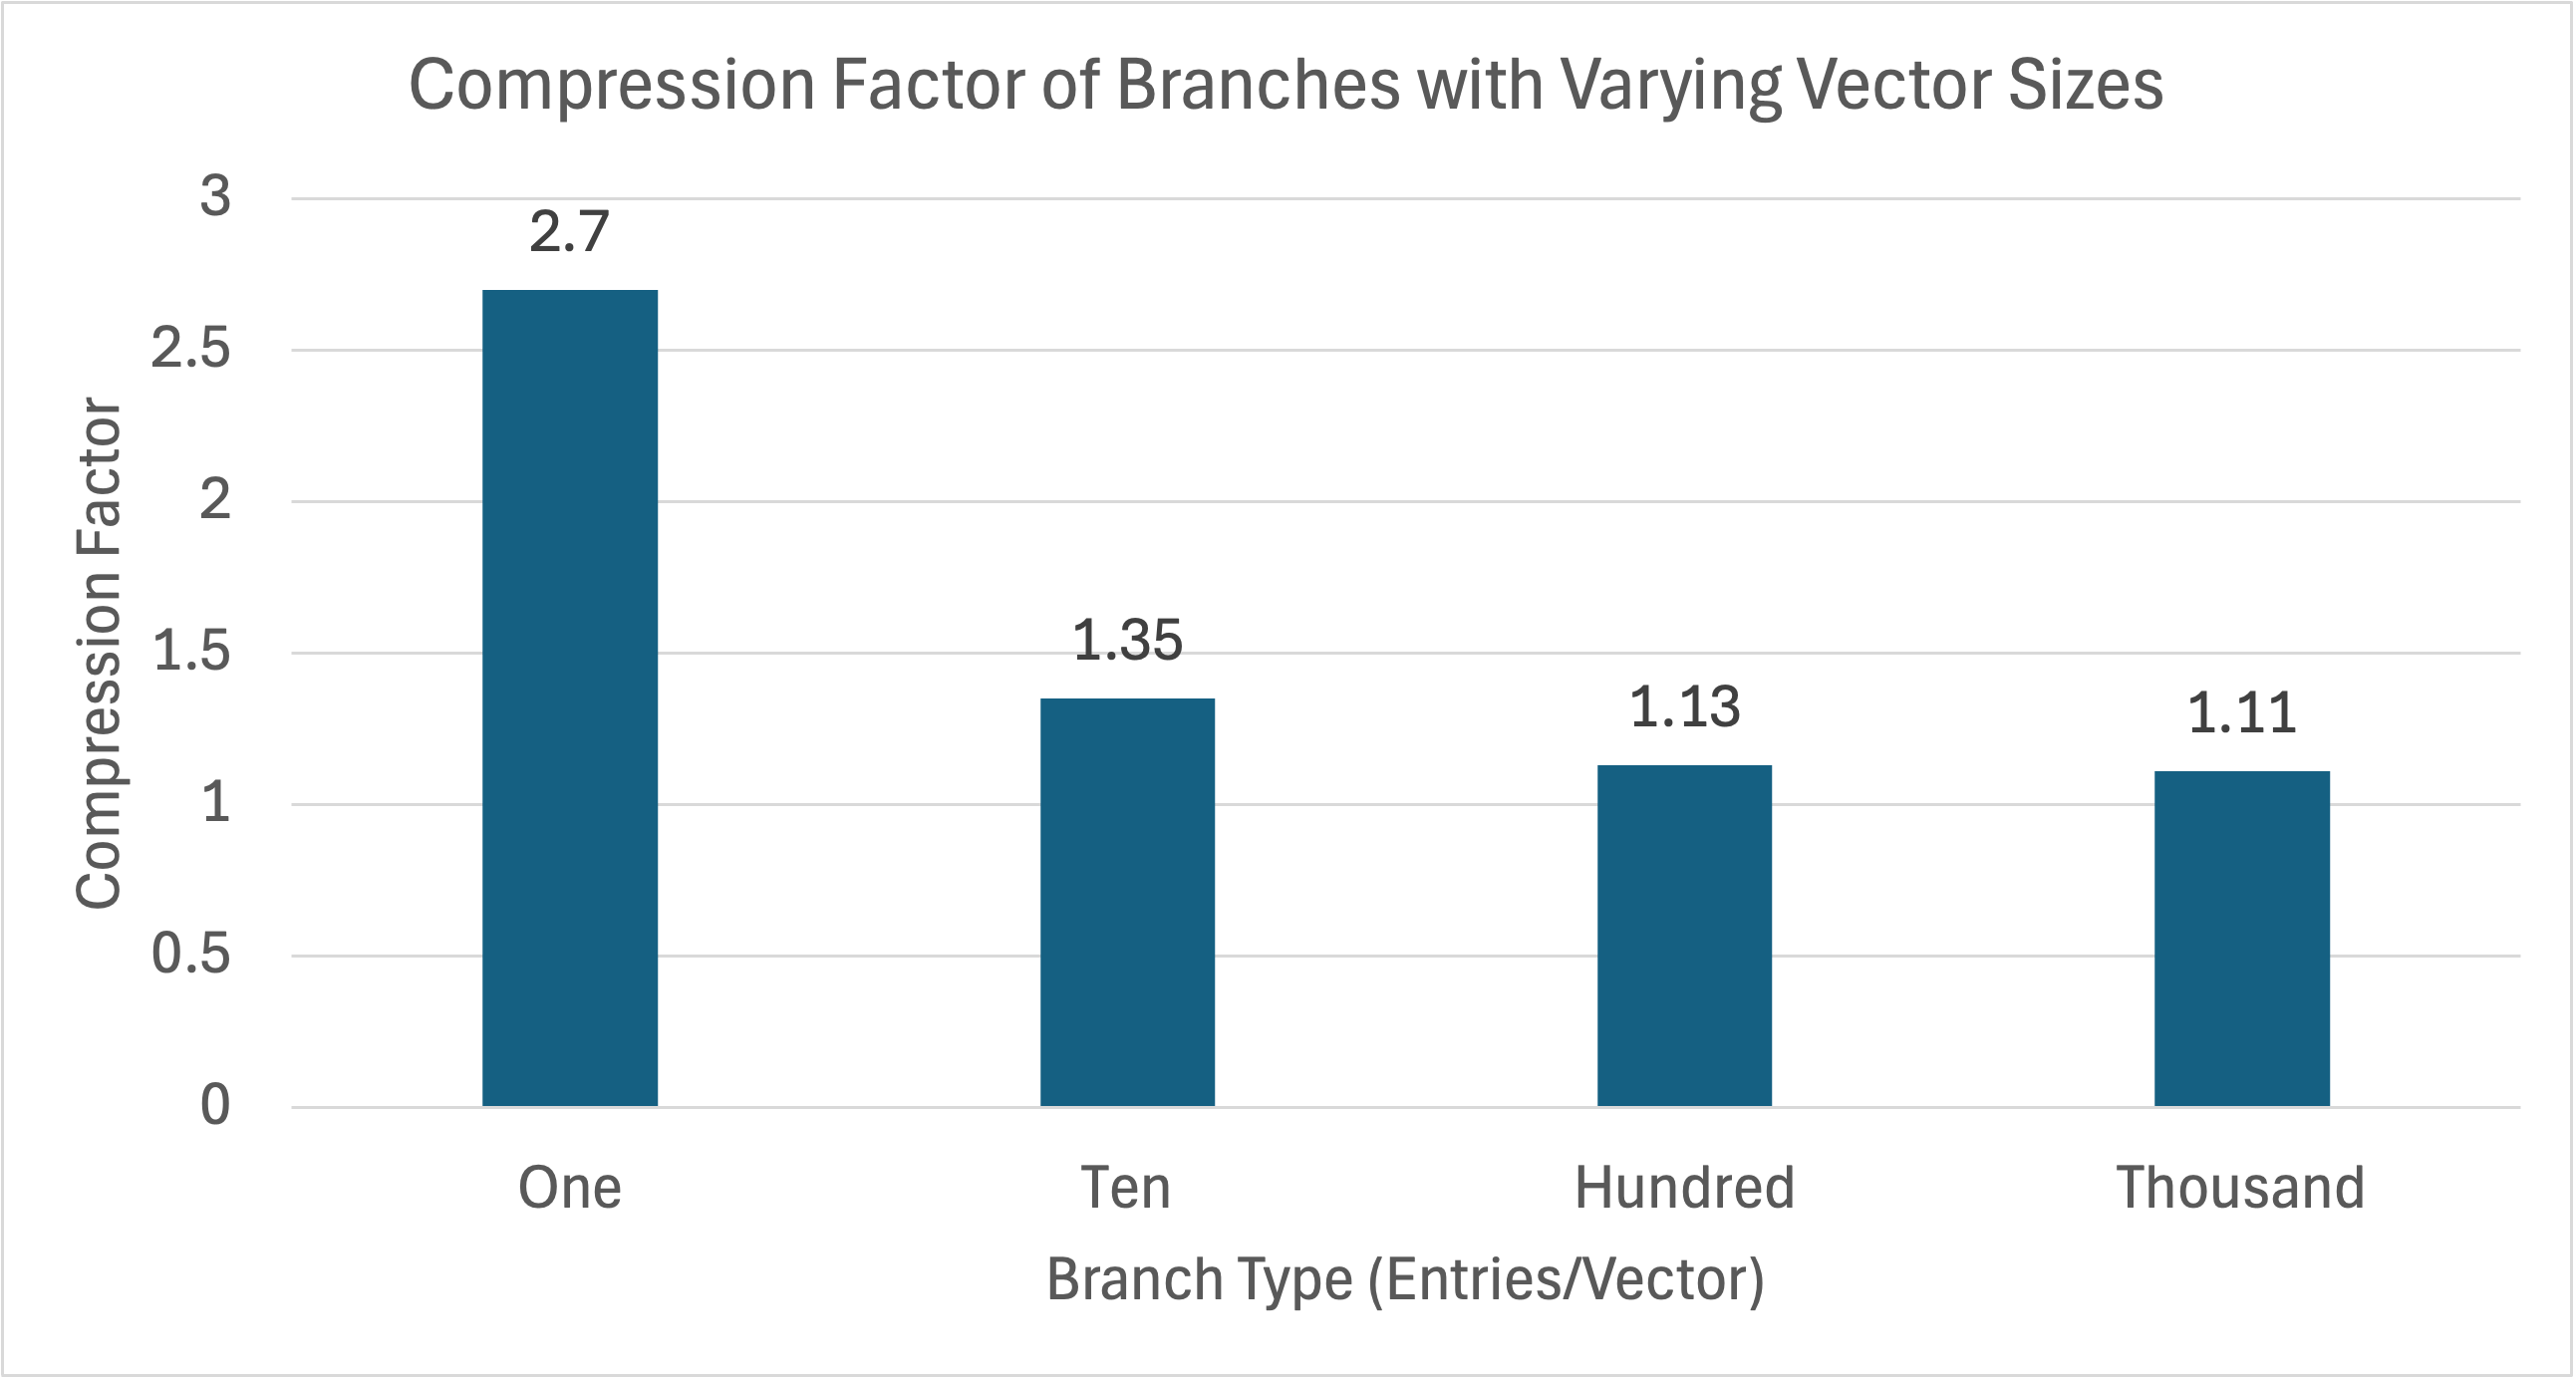
\includegraphics[width=.8\textwidth]{content/toymodel_content/branch_compfacts_nomix.png}
    \caption{Compression factors of $N=1000$ entries per branch with random-valued vectors of varying size.}
    \label{fig:toymodel_compF_rndm_vectors}
\end{figure}
\vspace{10px}

% \begin{figure}[h]
%     \caption{File size of $N=1000$ entries per branch with random-valued vectors of varying size.}
%     \label{fig:toymodel_filesize_rndm_vectors}
%     \centering
%     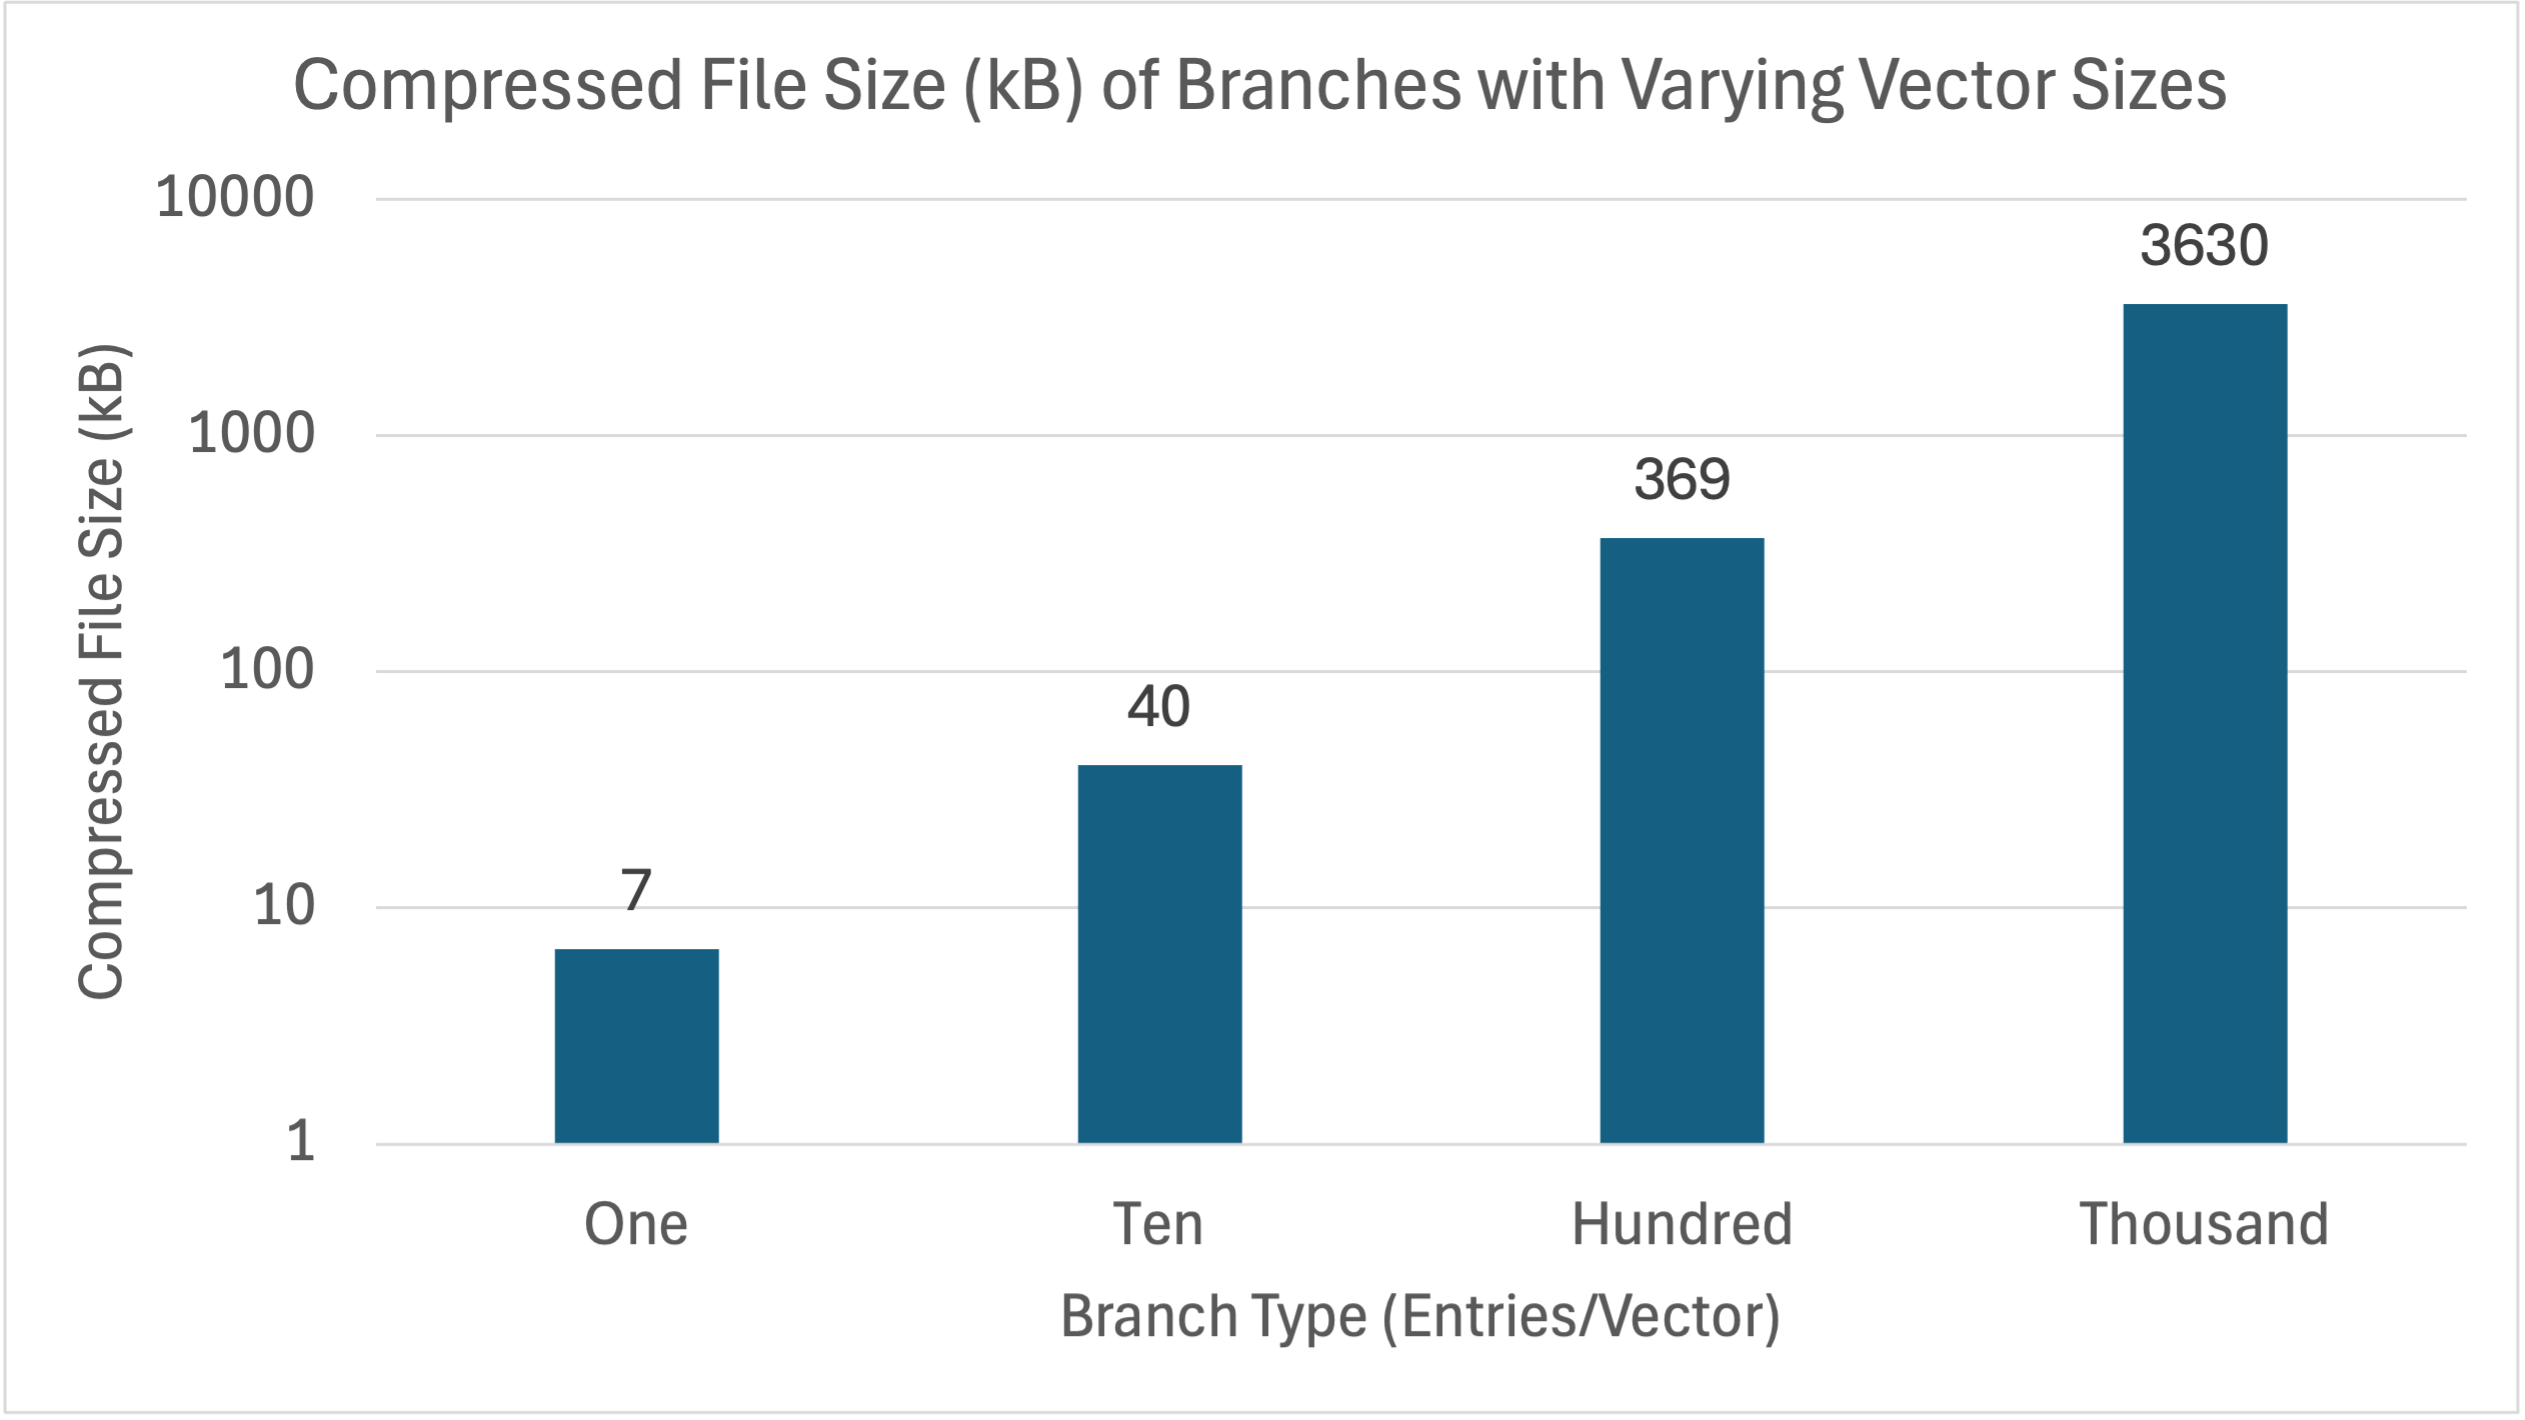
\includegraphics[width=.8\textwidth]{content/toymodel_content/branch_fileSize_nomix.png}
% \end{figure}


\subsection{Mixed-Random Float Branches}
The branches needed to have some balance between compressible and incompressible data to mimic the compression ratio found in real data.
How this was achieved was by filling each vector with different ratios of random floats and repeating integers, which will now be described in detail.

The first change was increasing the total number of events from $N = 10^4$ to $N = 10^5$. 
Mixing of random floats and repeated integer values takes the same script structure as Section \ref{sec:toy_compression_random_float_branches} but adjusts the event generation loop.

\begin{lstlisting}[language=C]  
  void VectorTree() {
    ...
    // Events Loop
    for (int j = 0; j < N; j++) {
        // Clearing entries from previous iteration
        vec_ten0.clear();
        vec_ten1.clear();
        vec_ten2.clear();
        vec_ten3.clear();

        // Generating vector elements, filling vectors
        // Generating vec_ten0
        // Contents of the vector:
        //    {float_0}
        //    Only one float of random value
        // And since there's only one entry, we don't mix the entries. 
        float_0 = gRandom->Gaus(0, 1) * gRandom->Rndm();
        vec_ten0.emplace_back(float_0);

        // Generating vec_ten1
        // Contents of the vector:
        //    {float_1_0, float_1_1, float_1_2, float_1_3, float_1_4, 1, 1, 1, 1, 1}
        //    5 floats of random values, 5 integers of value 1.
        for (int b = 0; b < size_vec_1; b++) {
            if (b < size_vec_1 / 2) {
              float_1 = gRandom->Rndm() * gRandom->Gaus(0, 1);
              vec_ten1.emplace_back(float_1);
            } else {
              float_1 = 1;
              vec_ten1.emplace_back(float_1);
            }
        }

        // Do the same with vec_ten2 and vec_ten3, except for 
        //     vectors with size 100 and 1000 respectively. 


        // After all branches are filled, fill the TTree with 
        //     new branches
        tree->Fill(); 
    }
    // Saving tree and file
    tree->Write();
    ...
  }
\end{lstlisting}

As shown in the \verb|if|-statements in line \verb|25|, if the iterator was less than half of the total number of entries in the vector then that entry had a randomized float put in that spot in the vector, otherwise it would be filled with the integer \verb|1|.
Having a mixture of half random floats and half integer \verb|1| led to the larger branches still seeing poor compression, so a new mixture of 1/4 random data was introduced. 
Even though $N=10^5$ had the larger branches closer to the desired compression ratio, testing at $N=10^6$ events improves the accuracy of the overall file size to more closely resemble real data.

Figure \ref{fig:toymodel_compF_1e6_mix_random} shows the difference between compression between the two mixtures at $N=10^6$ events. 
When the number of events is increased from $N=10^5$ to $N=10^6$, at the 1/2 random-mixture, the branches with more than one entry per vector see their compression factor worsen. 
Figure \ref{fig:toymodel_compF_1e5_mix_random} shows a compression ratio hovering around 3 for the larger branches, whereas Figure \ref{fig:toymodel_compF_1e6_mix_random} shows the same branches hovering around 2. 

\begin{figure}[h]
    \centering
    \vspace{20px}
    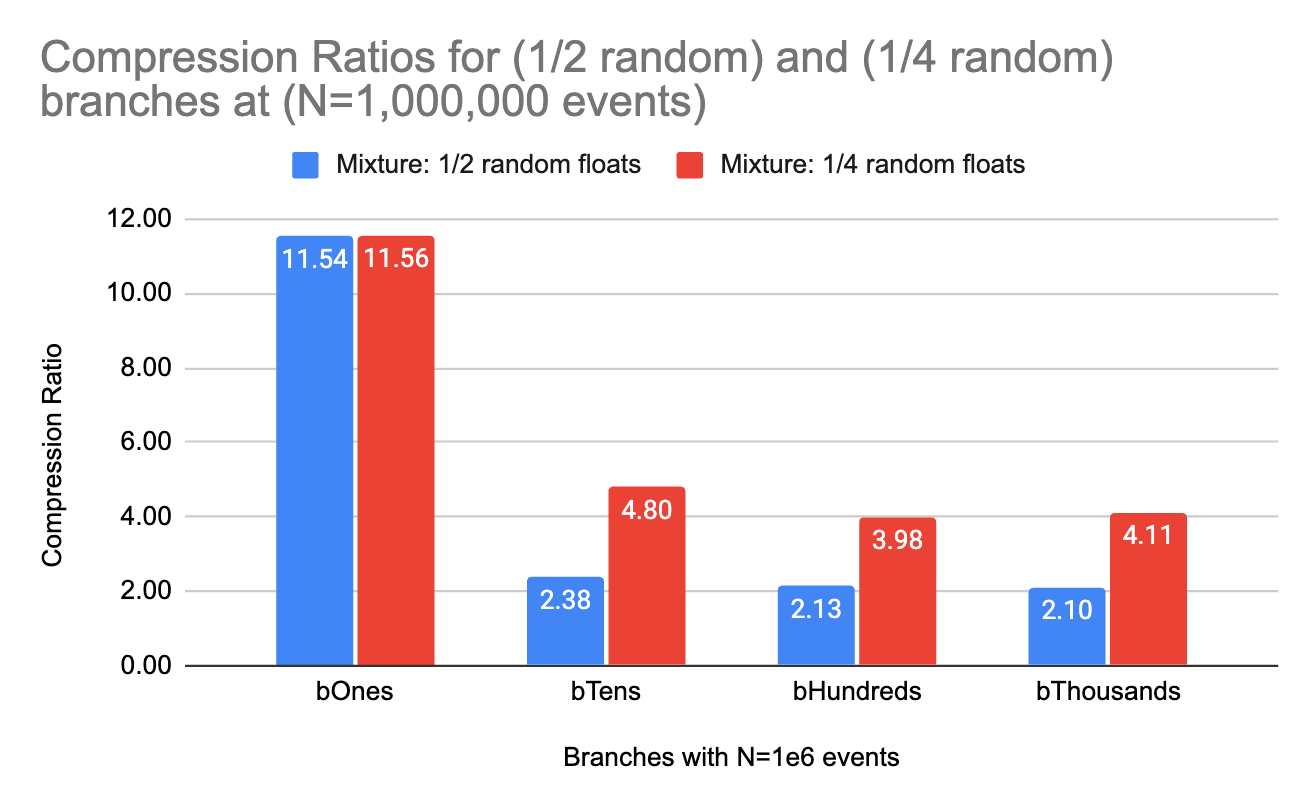
\includegraphics[width=.8\textwidth]{content/toymodel_content/Compression Ratios for (1_2 random) and (1_4 random) branches at (N=1,000,000 events).png}
    \caption{Compression Ratios for ($\frac{1}{2}$ random) and ($\frac{1}{4}$ random) branches at ($N=10^6$ events)}
    \vspace{20px}
    \label{fig:toymodel_compF_1e6_mix_random}
\end{figure}

\begin{figure}[h]
    \centering
    \vspace{20px}
    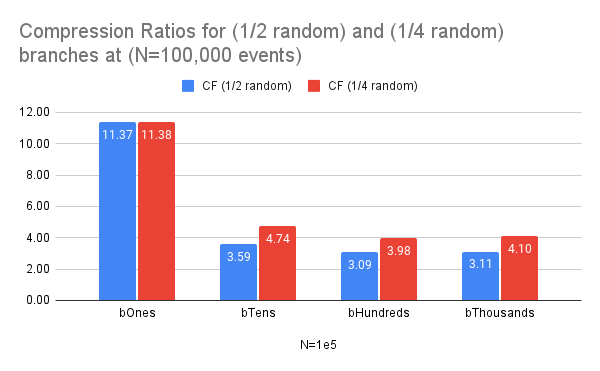
\includegraphics[width=.8\textwidth]{content/toymodel_content/Compression Ratios for (1_2 random) and (1_4 random) branches at (N=100,000 events).png}
    \caption{Compression Ratios for ($\frac{1}{2}$ random) and ($\frac{1}{4}$ random) branches at ($N=10^5$ events)}
    \vspace{20px}
    \label{fig:toymodel_compF_1e5_mix_random}
\end{figure}

Unlike the mixture of branches having 1/2 random data, the 1/4 mixture does not see the same compression effect, but with this mixture we see a compression ratio that is in-line with real data.
The more repeated integers within the mixture the easier it is to compress the branch, versus, the more random floating point numbers in the mixture more difficult the branch will be to compress.
With these mixtures added to the toy model, we can start looking at varying the basket sizes to see how they affect compression.

\section{Basket-Size Investigation}
\label{sec: toy-model basket-size investigation}

Investigating how compression is affected by the basket size requires us to change the basket size, refill the branch and read it out.
Changing the basket buffer size was done at the script level with a simple setting after the branch initialization and before the event loop the following code:
\pagebreak
\begin{lstlisting}
    int basketSize = 8192000; // 8 MB
    tree->SetBasketSize("*",basketSize);
\end{lstlisting}
This ROOT-level setting was sufficient for the case of the toy model; testing of the basket size setting both at the ROOT- and Athena-level would be done later using derivation production jobs in Section \ref{sec:DAODProd_Analysis}.
The lower bound set for the basket size was 1 kB and the upper bound was 16 MB.
The first branch looked at closely was the branch with a thousand vector-entries with half of them being random floats, see Figure \ref{fig:toymodel_CFvsBranchSize_1/2mixture}.

\begin{figure}[h]
    \centering
    \vspace{20px}
    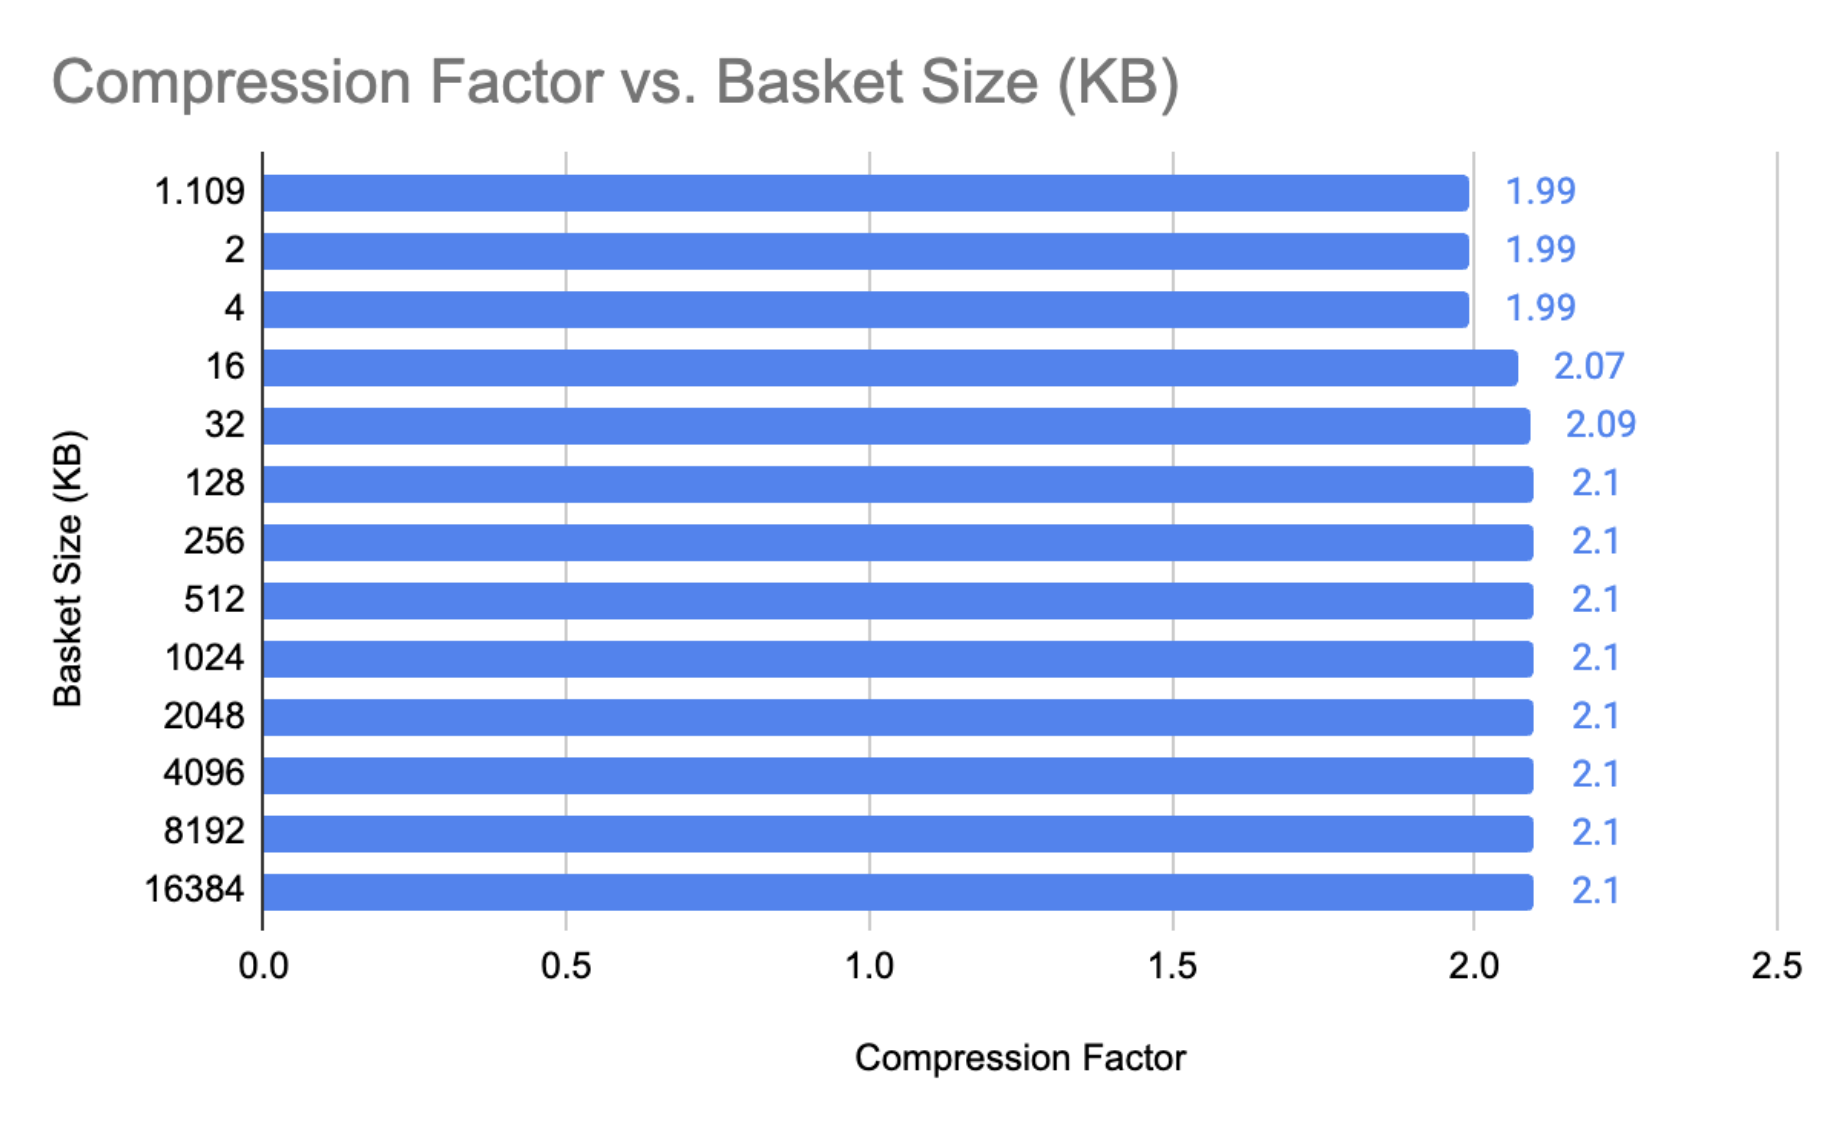
\includegraphics[width=.8\textwidth]{content/toymodel_content/Compression Factor vs. Branch Size (KB).png}
    \caption{Compression Factors vs Branch Size (1000 entries per vector, 1/2 Mixture $N=10^6$ events)}
    \vspace{20px}
    \label{fig:toymodel_CFvsBranchSize_1/2mixture}
\end{figure}

\begin{figure}[h]
    \centering
    \vspace{20px}
    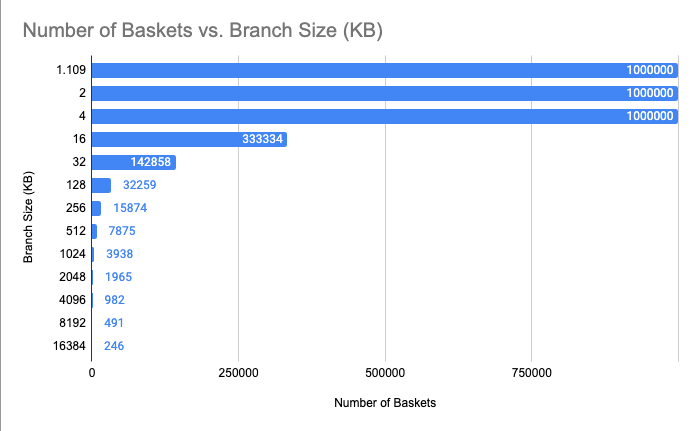
\includegraphics[width=.8\textwidth]{content/toymodel_content/Number of Baskets vs Branch Size.png}
    \caption{Number of Baskets vs Branch Size (1000 entries per vector, 1/2 Mixture $N=10^6$ events)}
    \vspace{20px}
    \label{fig:toymodel_NumBasketsvsBranchSize_1/2mixture}
\end{figure}

Figures \ref{fig:toymodel_CFvsBranchSize_1/2mixture} and \ref{fig:toymodel_NumBasketsvsBranchSize_1/2mixture} are the first indication that the lower basket sizes are too small to effectively compress the data. 
For baskets smaller than 16 kB, it is necessary to have as many baskets as events to store all the data effectively.
For a mixed-content vector with one thousand entries, containing 500 floats and 500 integers (both are 4 bytes each), its size is approximately 4 kB.
ROOT creates baskets of at least the size of the smallest branch entry, in this case the size of a single vector.
So even though the basket size was set to 1 or 2 kB, ROOT created baskets of 4 kB.
These baskets less than or equal to $4$kB have a significantly worse compression than the baskets greater than $4$kB in size, so the focus was shifted toward baskets.  
Once the basket size is larger than the size of a single vector, more than one vector can be stored in a single basket and the total number of baskets is reduced.

There were different types of configuration to the toy model investigated by this study. 
Looking further into the types of mixtures and how they would affect compression are shown in Figures \ref{fig:toymodel_328_compF_vs_basketsize} and \ref{fig:toymodel_418_compF_vs_basketsize}. 
Here the same mixtures were used but the precision of the floating point numbers was decreased from the standard 32 floating-point precision to 16 and 8, making compression easier. 

\begin{figure}[h]
    \centering
    \vspace{20px}
    \begin{subfigure}{.5\textwidth}
        \centering
        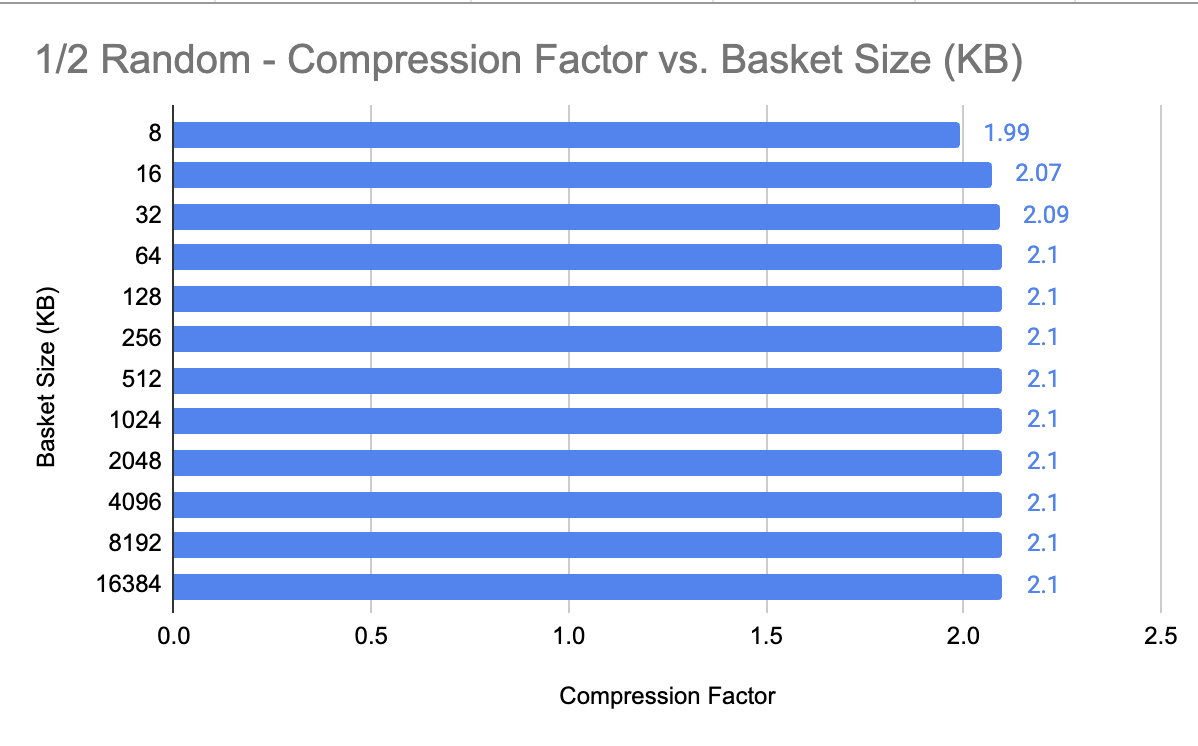
\includegraphics[width=\textwidth]{content/toymodel_content/3.28/1_of_2.png}
        % \caption{A subfigure}
        \label{fig:toymodel_328_compF_vs_basketsize_subA}
      \end{subfigure}%     
      \begin{subfigure}{.5\textwidth}
        \centering
        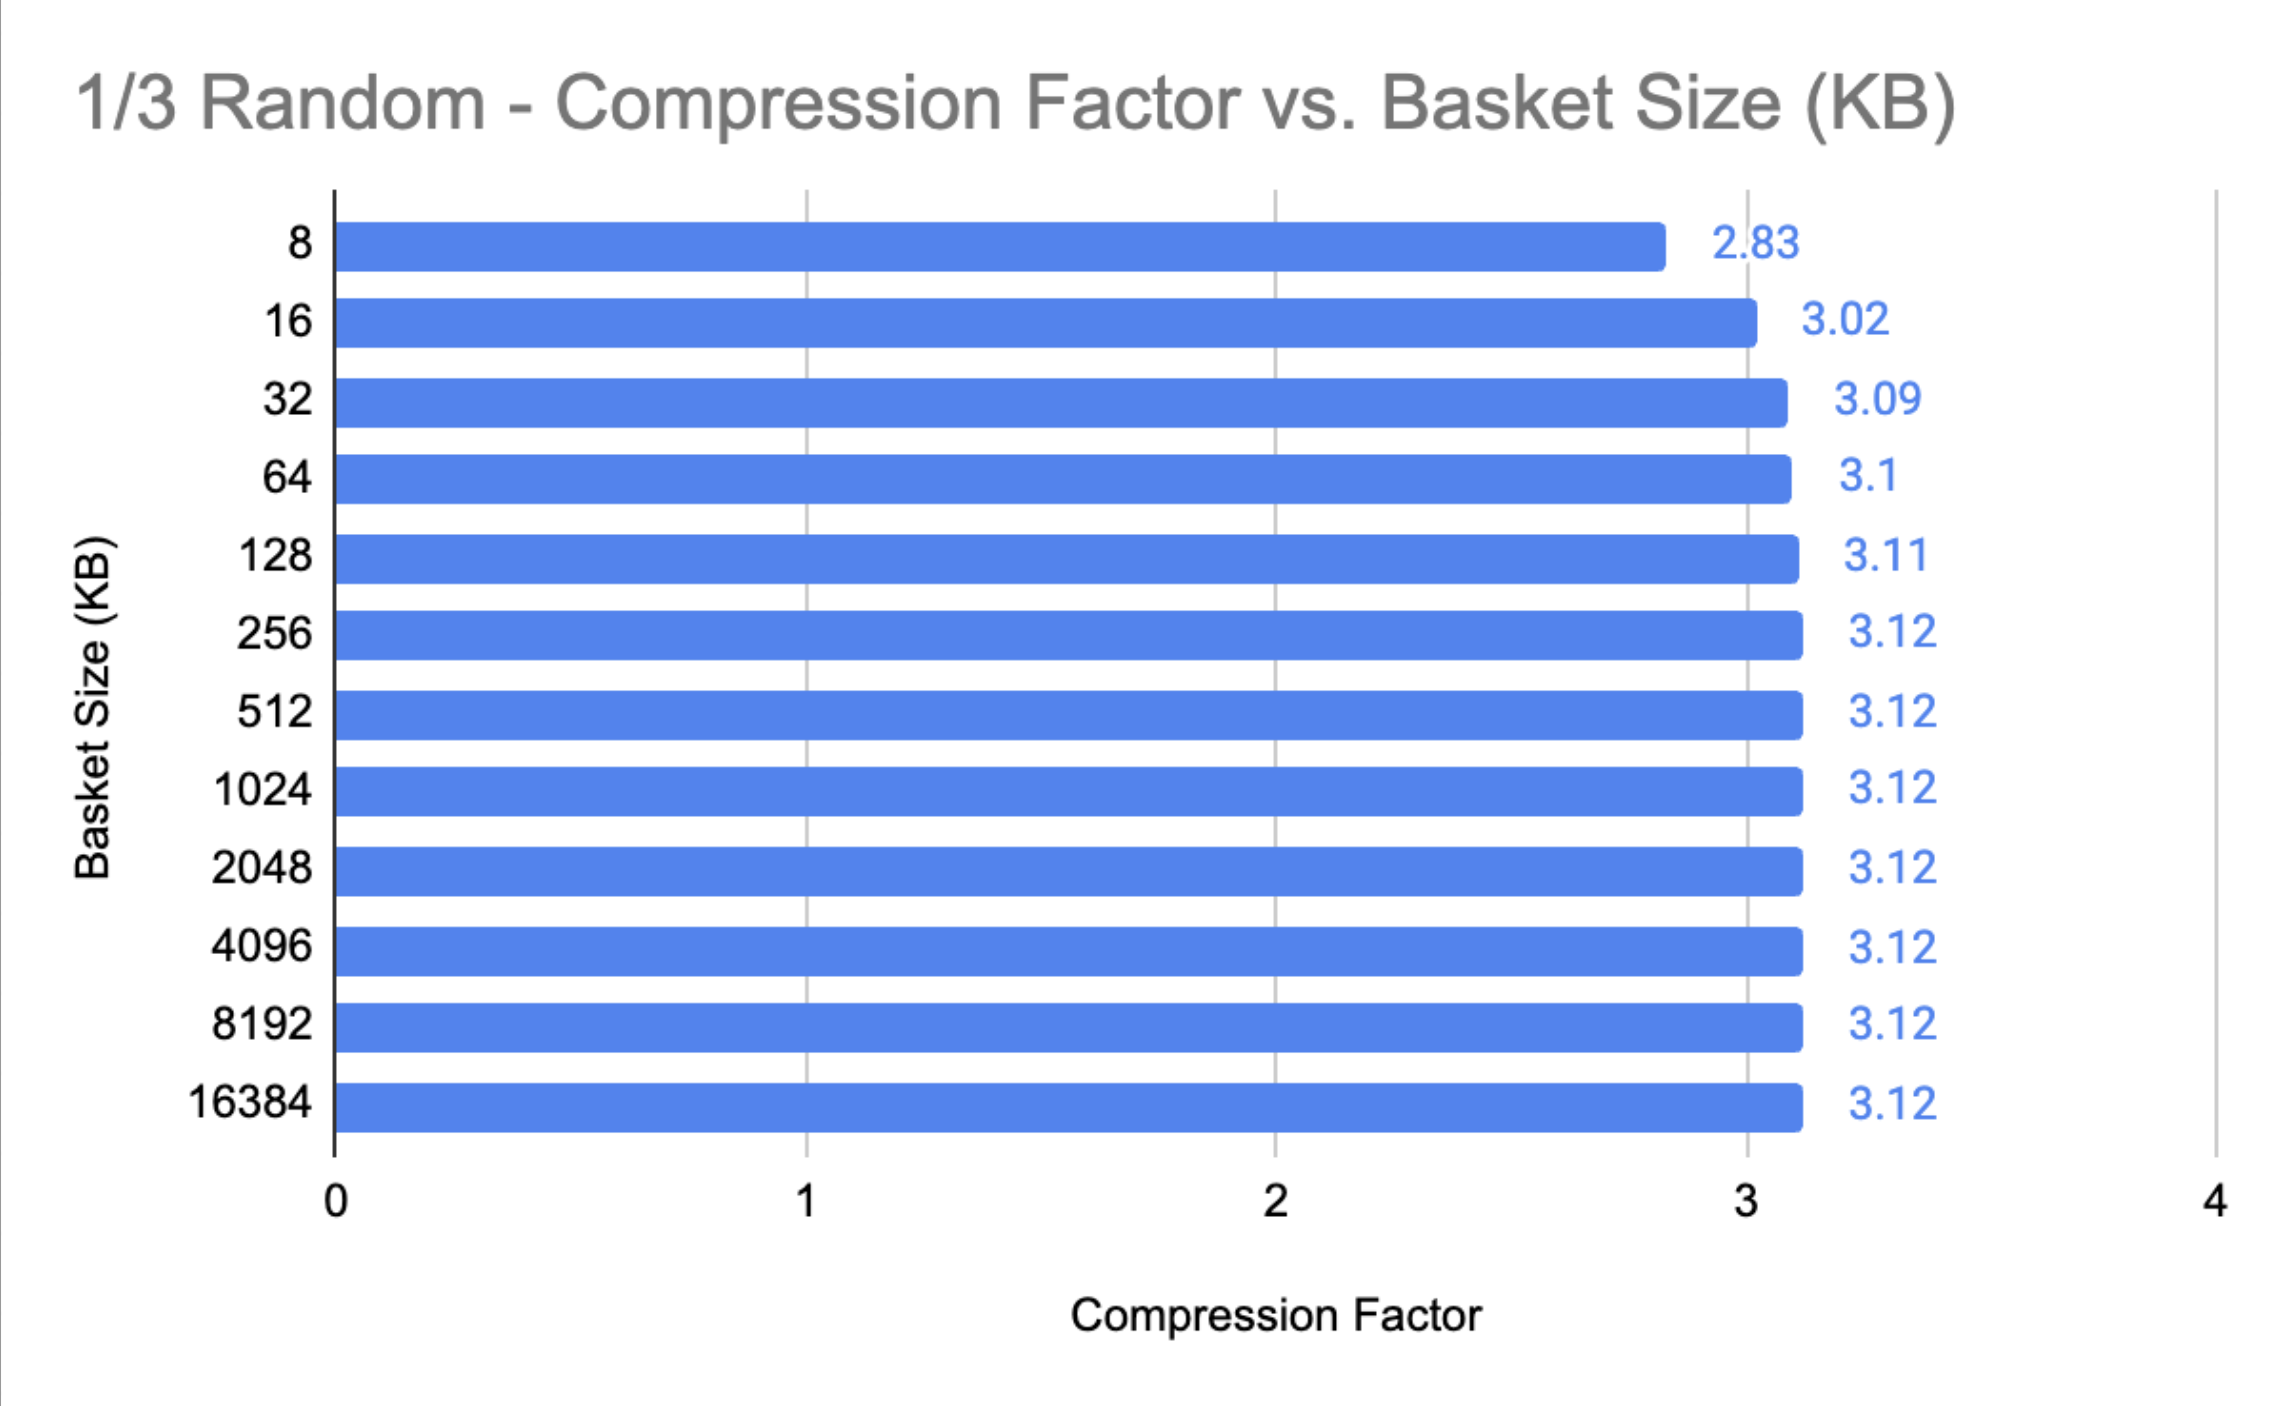
\includegraphics[width=\textwidth]{content/toymodel_content/3.28/1_of_3.png}
        % \caption{B subfigure}
        \label{fig:toymodel_328_compF_vs_basketsize_subB}
      \end{subfigure}% 
      \linebreak
      \begin{subfigure}{.5\textwidth}
        \centering
        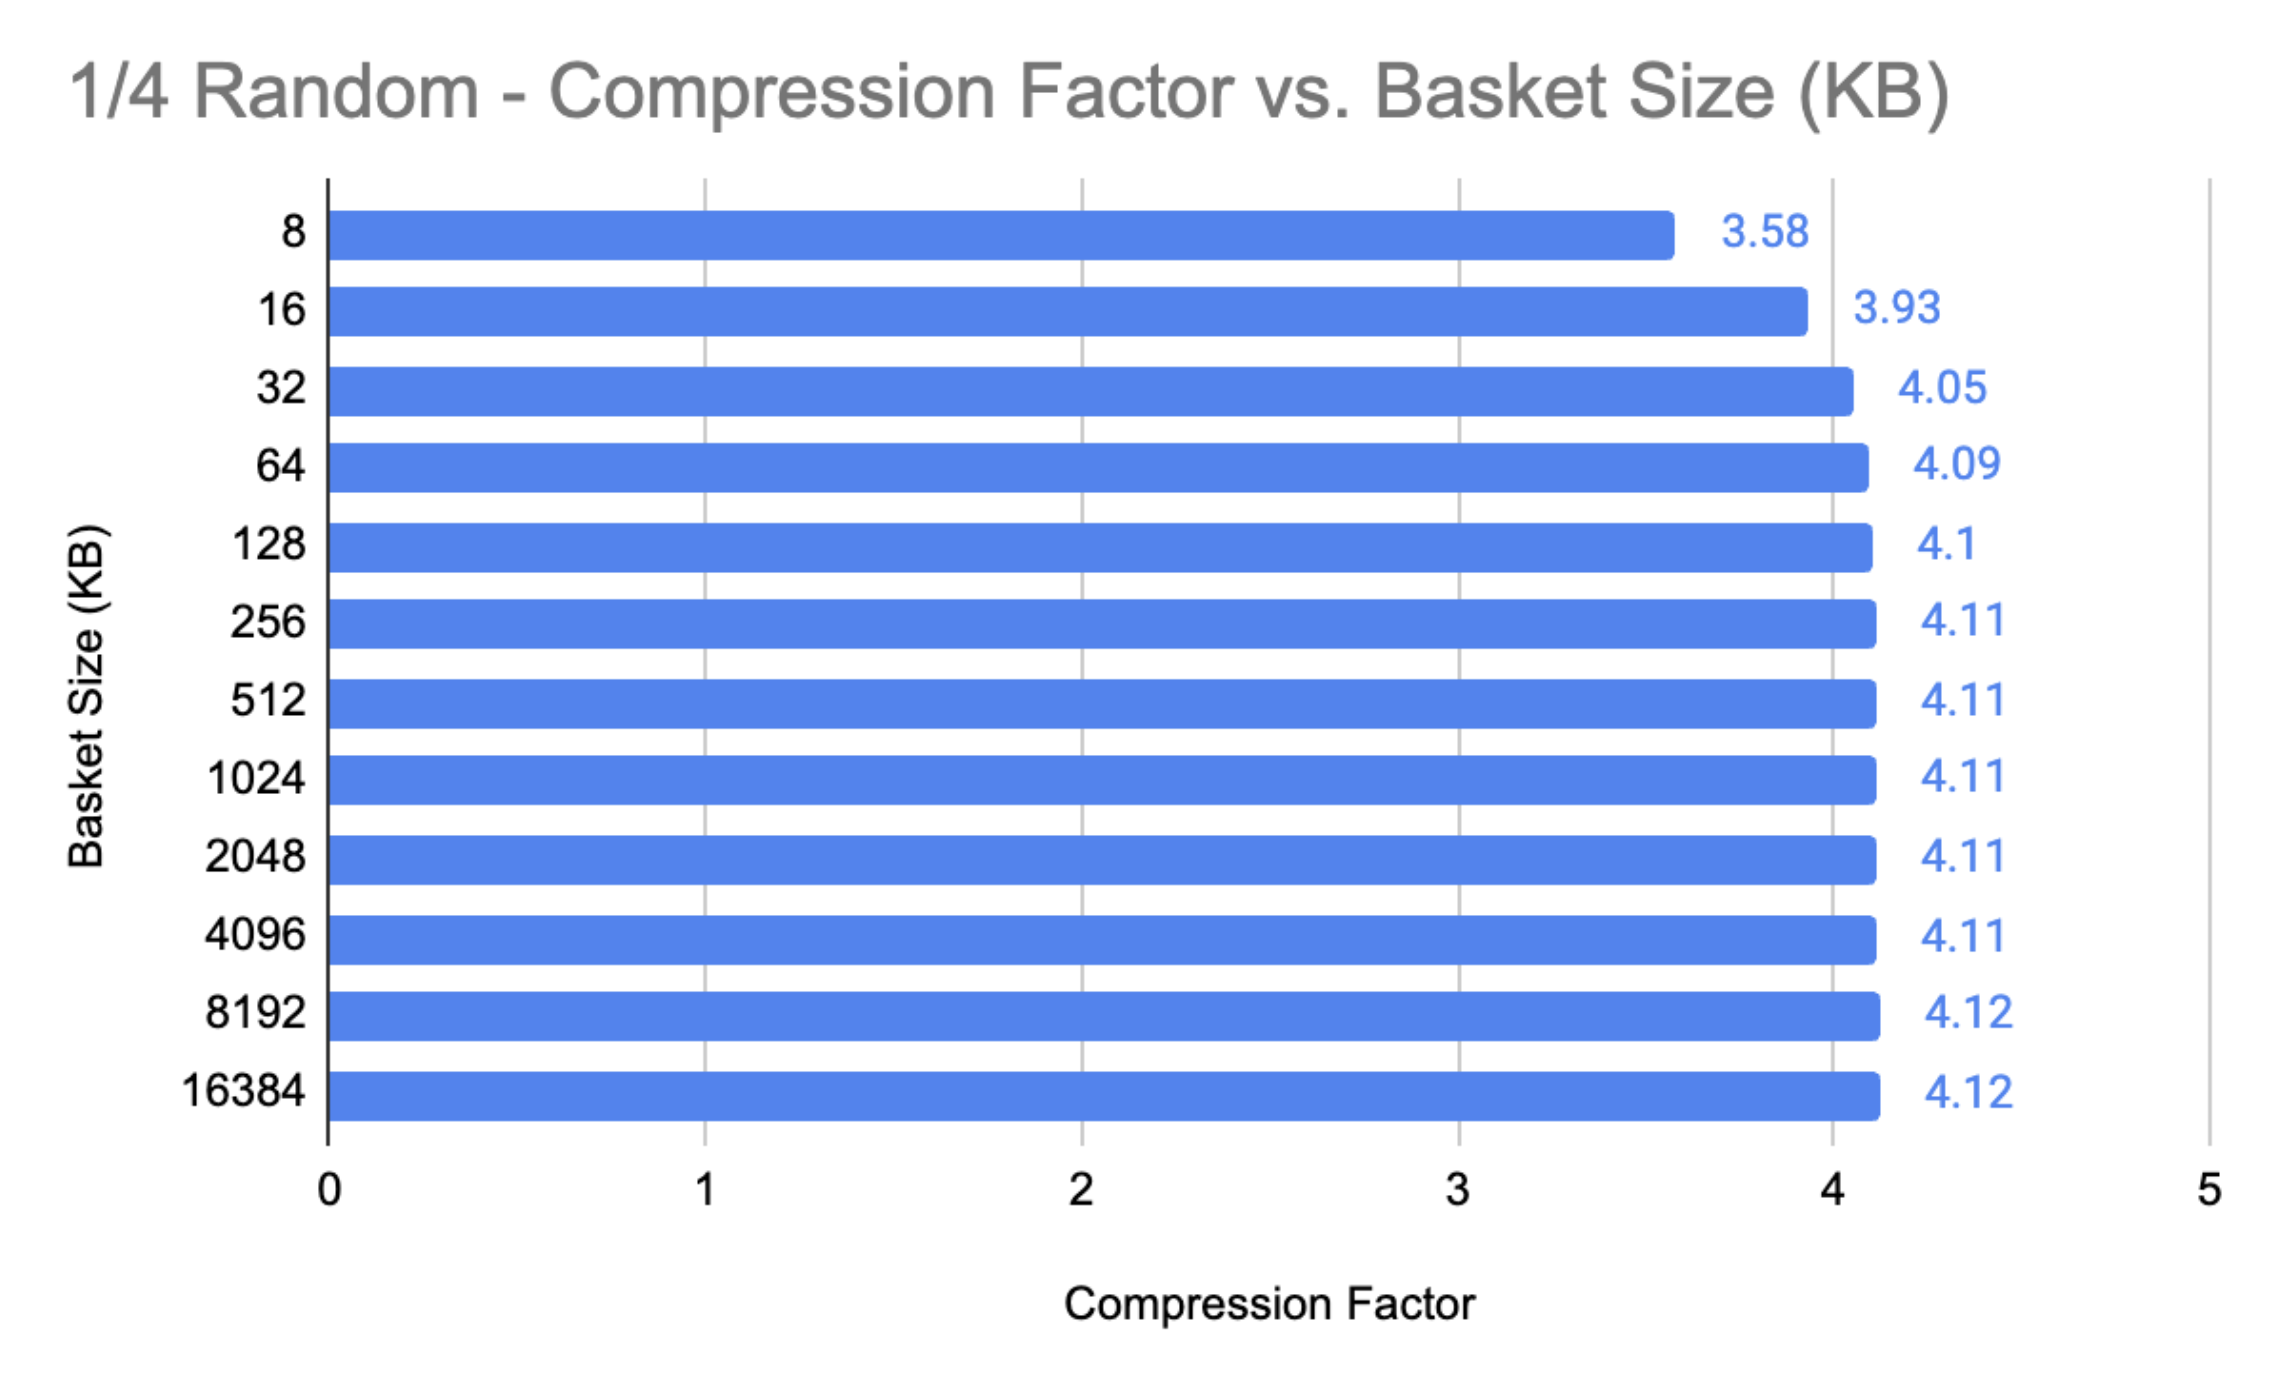
\includegraphics[width=\textwidth]{content/toymodel_content/3.28/1_of_4.png}
        % \caption{C subfigure}
        \label{fig:toymodel_328_compF_vs_basketsize_subC}
      \end{subfigure}% 
      \begin{subfigure}{.5\textwidth}
        \centering
        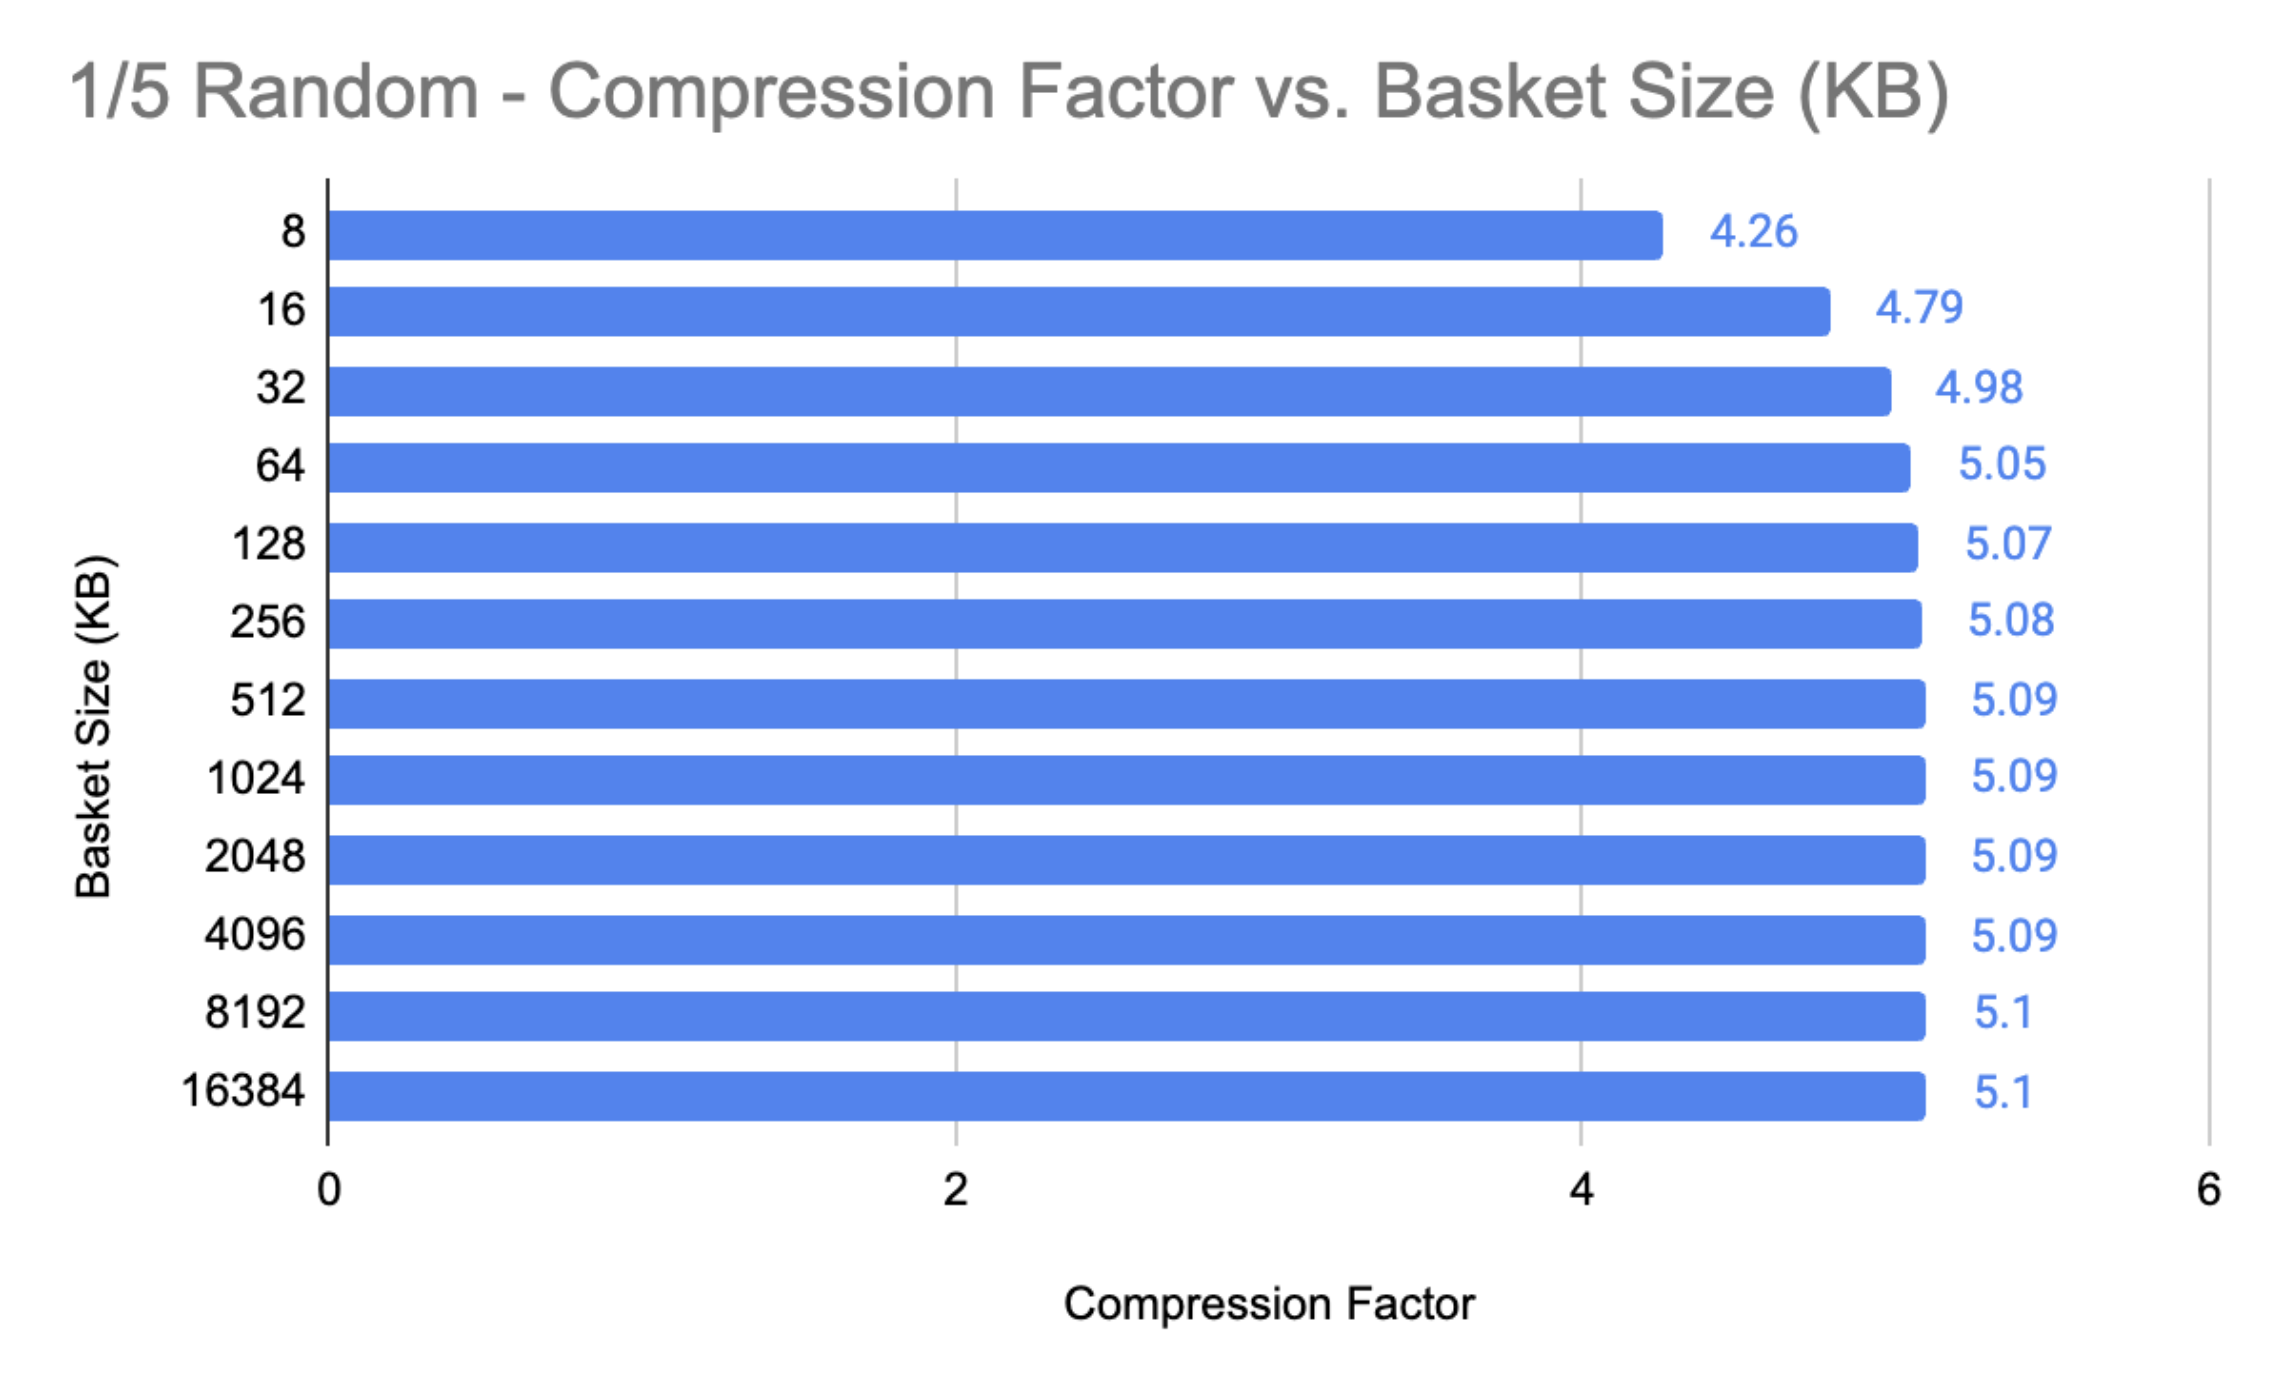
\includegraphics[width=\textwidth]{content/toymodel_content/3.28/1_of_5.png}
        % \caption{D subfigure}
        \label{fig:toymodel_328_compF_vs_basketsize_subD}
      \end{subfigure}% 
    \caption{Varying Mixtures in 8 point precision - Number of Baskets vs Branch Size ($N=10^6$ events)}
    \vspace{20px}
    \label{fig:toymodel_328_compF_vs_basketsize}
\end{figure}

\begin{figure}[h]
    \centering
    \begin{subfigure}{.5\textwidth}
        \centering
        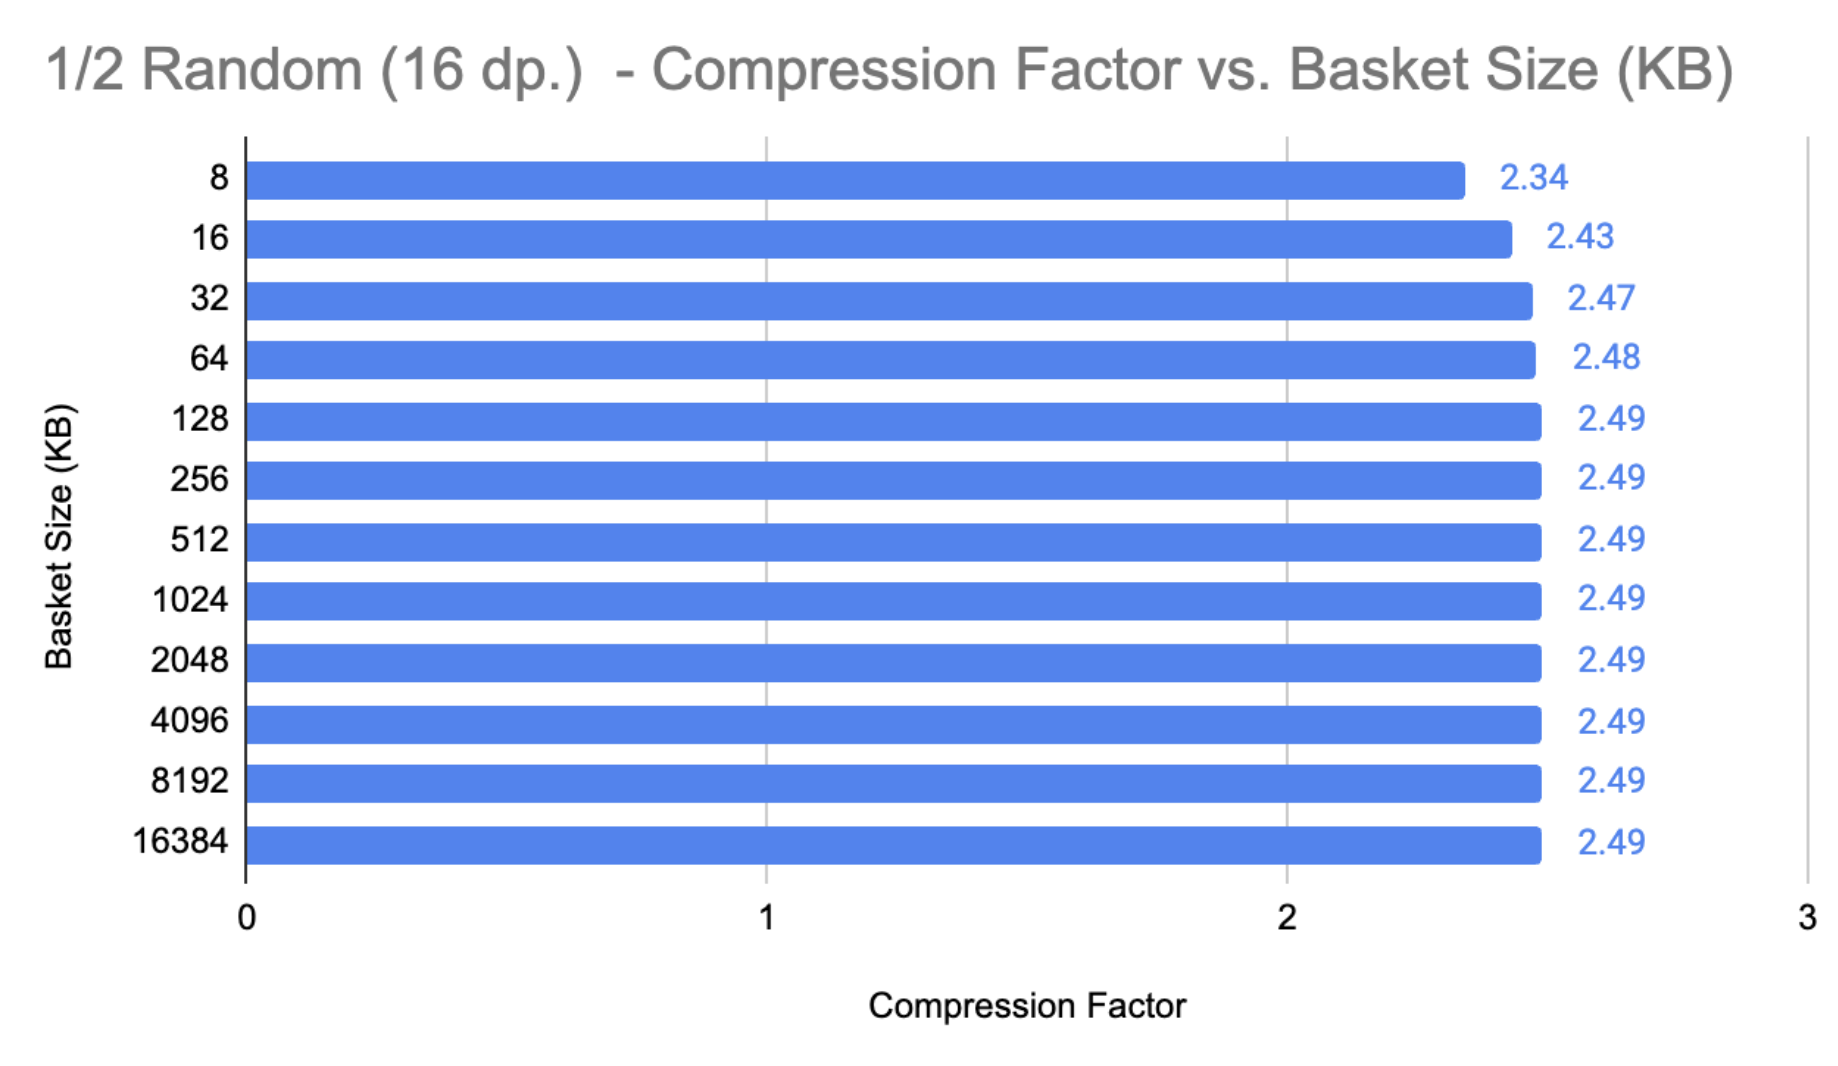
\includegraphics[width=\textwidth]{content/toymodel_content/4.18/1_of_2.png}
        % \caption{A subfigure}
        \label{fig:toymodel_418_compF_vs_basketsize_subA}
      \end{subfigure}%     
      \begin{subfigure}{.5\textwidth}
        \centering
        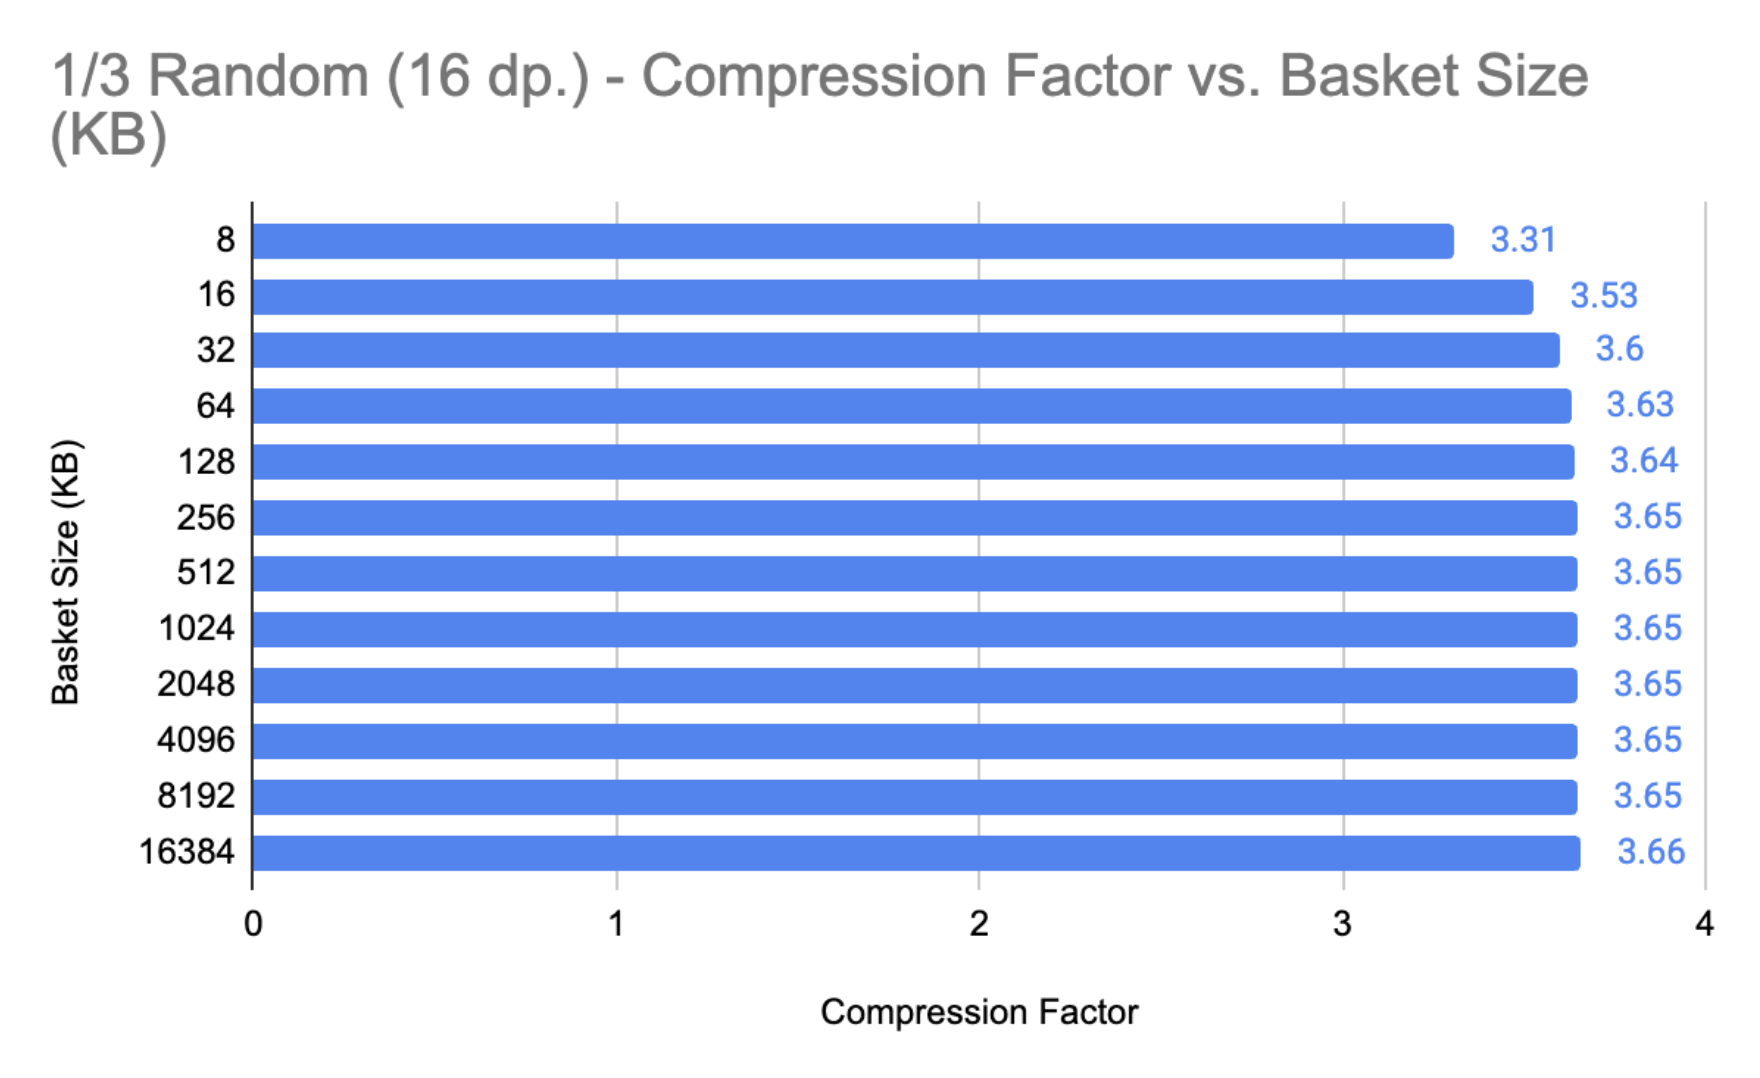
\includegraphics[width=\textwidth]{content/toymodel_content/4.18/1_of_3.png}
        % \caption{B subfigure}
        \label{fig:toymodel_418_compF_vs_basketsize_subB}
      \end{subfigure}% 
      \linebreak
      \begin{subfigure}{.5\textwidth}
        \centering
        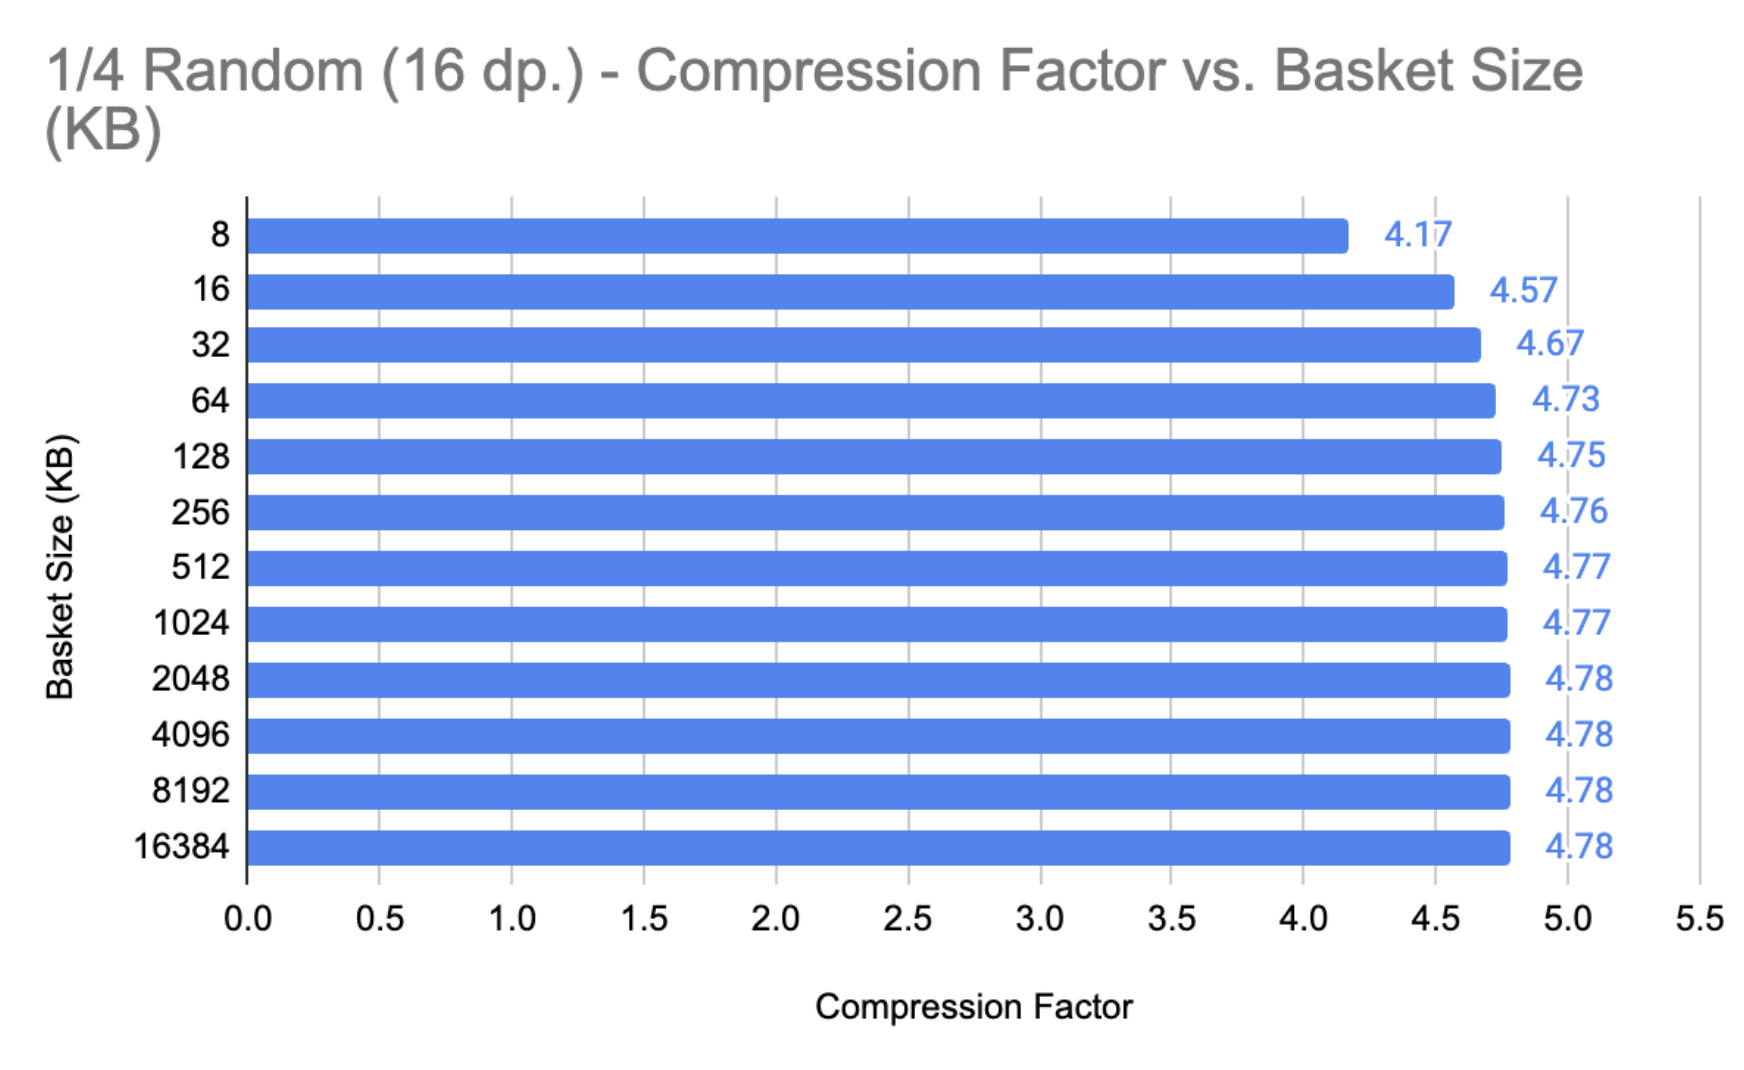
\includegraphics[width=\textwidth]{content/toymodel_content/4.18/1_of_4.png}
        % \caption{C subfigure}
        \label{fig:toymodel_418_compF_vs_basketsize_subC}
      \end{subfigure}% 
      \begin{subfigure}{.5\textwidth}
        \centering
        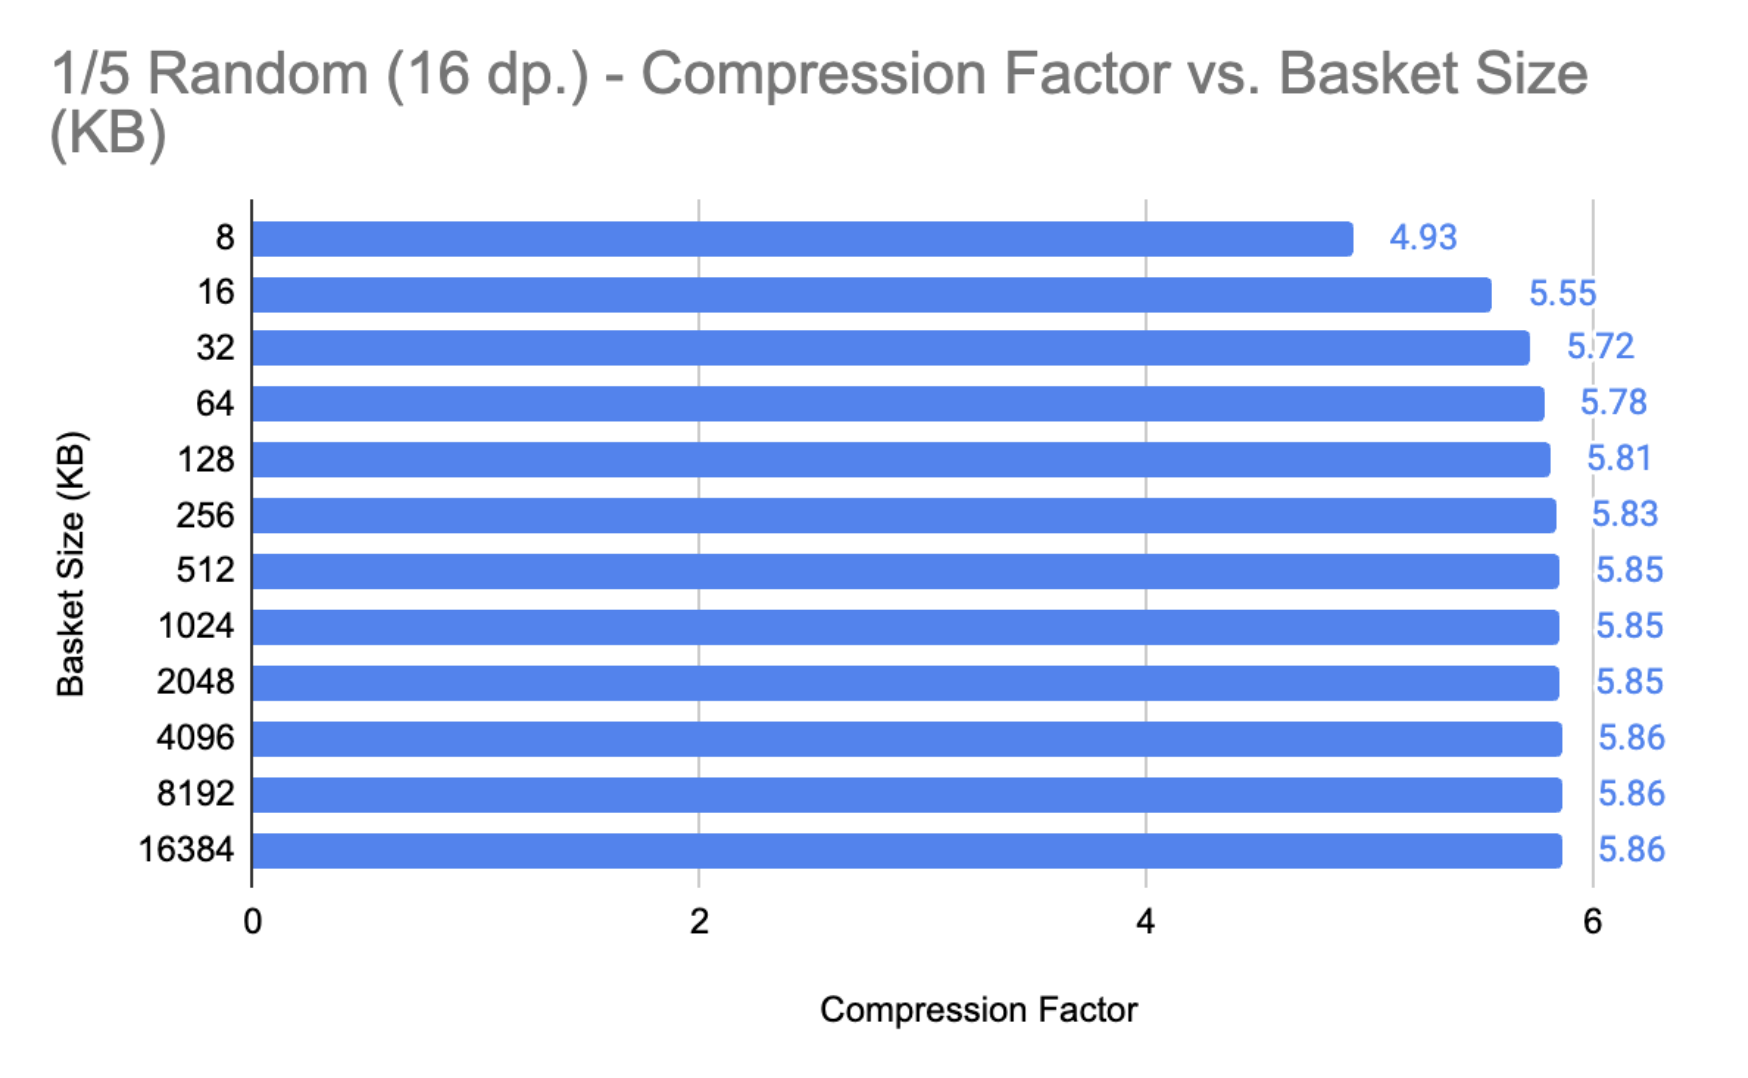
\includegraphics[width=\textwidth]{content/toymodel_content/4.18/1_of_5.png}
        % \caption{D subfigure}
        \label{fig:toymodel_418_compF_vs_basketsize_subD}
      \end{subfigure}% 
      \caption{Varying Mixtures in 16 point precision - Number of Baskets vs Branch Size ($N=10^6$ events)}
      \label{fig:toymodel_418_compF_vs_basketsize}
\end{figure}


Each of these sets of tests indicate that after a certain basket size, i.e. 128 kB, there is no significant increase in compression. 
Having an effective compression at 128 kB, it's useful to stick to that basket size to keep memory usage down. 
Knowing that increasing the basket size beyond 128 kB yields diminishing returns, it's worth moving onto the next phase of testing with actual derivation production jobs.



% 4. Real DAOD Jobs 
% -- 
\chapter{Data and Monte Carlo Derivation Production}
\label{chap:DAODProd}
Derivation production demands high memory usage, and DAODs make up a bulk of disk-space usage. 
DAODs are used in physics analyses and ought to be optimized to alleviate stress on the GRID and to lower disk-space usage. 
Optimizing both disk-space and memory usage is a tricky balance as they are typically at odds with one another. 
For example, increasing memory output memory buffers results in lower disk-space usage due to better compression but the memory usage will increase since the user will load a larger buffer into memory. 
This project opted to take is by optimizing for disk-space and memory by testing various basket limits and viewing the effects of the branches on both data and Monte Carlo (MC) simulated analysis object data (AODs).

\section{Basket-size Configuration}
\label{sec:DAODProd_Analysis}
% RSS/PSS for memory usage and output file size for disk usage

As the toy model ruled out, the focus here was on optimizing Athena and not ROOTs contribution for optimization.
The initial focus was on the inclusion of a minimum number of entries per buffer and the maximum basket buffer limit.
The AthenaPOOL script directly involved with these buffer settings is the \verb|PoolWriteConfig.py| found in the path \verb|athena/Database/AthenaPOOL/AthenaPoolCnvSvc/python/|.
As discussed in Section \ref{sec:DAODProd_Results}, further testing opted to keep the minimum number of entries set to its default setting, 10 entries per buffer. 

Throughout the duration of this testing, the results of compression or file size are independent of any changes to the release or the nightly version of Athena.  
The data derivation job comes from a 2022 dataset with four input files and 160,327 events. 
The MC job comes from a 2023 $t\bar{t}$ standard sample simulation job with six input files and 140,000 events. 
The datasets are noted in Appendix \ref{app: deriv job dataset}.

\subsection{Derivation Job Configuration}
To run a derivation job for testing purposes, AODs need to be downloaded by a data-management service, such as Rucio, to a machine dedicated to manually run tests.\cite{RUCIO_citation} 
Rucio is the data-management solution used for this project to procure the various AOD input files used for the derivation jobs.
The machine running the Rucio client will need to have a valid proxy added for Rucio to run correctly.  

A sample command would look like:
\begin{lstlisting}[language=bash]
rucio download data22_13p6TeV:AOD.31407809._000898.pool.root.1
\end{lstlisting}
This downloads the AOD file from Rucio and saves it to the user's local directory.

The command used by Athena to run a derivation job takes the form of the following example: 
\begin{lstlisting}[language=bash]
ATHENA_CORE_NUMBER=4 Derivation_tf.py \
--CA True \
--inputAODFile mc23_13p6TeV.601229.PhPy8EG_A14_ttbar_hdamp258p75_SingleLep.merge.AOD.e8514_e8528_s4162_s4114_r14622_r14663/AOD.33799166._001224.pool.root.1 \
--outputDAODFile art.pool.root \
--formats PHYSLITE \
--maxEvents 2000 \
--sharedWriter True \
--multiprocess True ;  
\end{lstlisting}
Where Athena allows one to specify the number of cores to use with the \verb|ATHENA_CORE_NUMBER| environment variable.
\verb|Derivation_tf.py| is a script that runs the derivation job and is part of the Athena release.
The \verb|--inputAODFile| is the input file for the derivation job, in this case an AOD file.
The user can specify multiple input files at a time by enclosing the input files in quotes and separating each file with a comma, like the following:
\begin{lstlisting}[language=bash]
    --inputAODFile="AOD.A.pool.root.1,AOD.B.pool.root.1,AOD.C.pool.root.1,AOD.D.pool.root.1"
\end{lstlisting}
The \verb|--outputDAODFile| is the output file for the derivation job, in this case a DAOD file.
The \verb|--formats PHYSLITE| flag allows the job to use the PHYSLITE format for the DAOD.
Here is where the user may choose to include PHYS or PHYSLITE simply by inlusion of one or both.
The \verb|--maxEvents| flag allows one to specify the maximum number of events to run the job on.
The \verb|--multiprocess True| flag allows the job to use AthenaMP tools.
AthenaMP is a mode of operation that allows for multi-process parallelism in many workflows since Run 2.\cite{SerhanMete:20223X} 
The \verb|--sharedWriter True| flag allows the job to utilize SharedWriter, which is a memory allocation mechanism as part of AthenaMP which allows for multiple workers to share allocated memory in the writing process. 
The machine used to run these derivation tests was a CERN based machine, using an $\textsc{AMD EPYC}$ 7302 16-Core Processor, supplied with 258 GB of memory, on version 9.4 of the AlmaLinux distribution. 


The input files for both data and MC jobs were ran with various configurations of Athena by modifying the basket buffer limit. 
The four configurations tested all kept minimum number of basket buffer entries at 10 and modified the basket limitation in the following ways: 

\begin{enumerate}
    \item ``$\textit{default}$" - Athena's default setting, and basket limit of 128 kB
    \item ``$\textit{256k}$'' - Limit basket buffer to 256 kB
    \item ``$\textit{512k}$'' - Limit basket buffer to 512 kB
    \item ``$\textit{no-lim}$'' - Removing the Athena basket limit, the ROOT imposed 1.3 MB limit still remains
\end{enumerate}

% ====== 
% RESULTS
% ======

\section{Results}
\label{sec:DAODProd_Results}

\subsection{Presence of basket-cap and presence of minimum number of entries}
\label{sec:DAODProd_Results_presence}

The first batch testing was for data, Table \ref{Tab: night-data-outputfs}, and MC simulation, Table \ref{Tab: night-mc-outputfs}, derivation production jobs with and without presence of an upper limit to the basket size and presence of the minimum number of basket buffer entries. 
PHYSLITE MC derivation production, from Table \ref{Tab: night-mc-outputfs}, sees a 9.9\% increase in output file size when compared to the default Athena configuration. 
Since this configuration only differs by the omission of the ``min-number-entries" requirement, we assume the minimum number of basket buffer entries should be kept at 10 and left alone. 

\vspace{15px}

% Data file sizes 
% Athena version: Nightly from v22.0.16 
% input file: # TODO
% PHYS/PHYSLITE

\begin{table}[!ht]
    \centering
    \resizebox{\textwidth}{!}{
        \begin{tabular}{|c|c|c|c|}
            \hline
                Presence of features (Data) & Max PSS (MB) ($\Delta$\% default) & PHYS outFS (GB) ($\Delta$\%) & PHYSLITE outFS (GB) ($\Delta$\%) \\ \hline
                basket-cap, min-num-entries (default)  & 27.1 ( + 0.0 \%) & 3.22 ( + 0.0 \%) & 1.03 ( + 0.0 \%) \\ \hline
                \st{basket-cap} \st{min-num-entries} & 27.8 ( + 2.5 \%) & 3.22 ( + 0.2 \%) & 1.04 ( + 0.2 \%) \\ \hline
                \st{basket-cap} min-num-entries & 27.8  ( + 2.5 \%) & 3.22 ( - 0.0 \%) & 1.03 ( - 0.4 \%) \\ \hline
                basket-cap,  \st{min-num-entries} & 27.3 ( + 0.7 \%) & 3.22 ( + 0.2 \%) & 1.04 ( + 0.7 \%) \\ \hline
            \end{tabular}
    }
    \label{Tab: night-data-outputfs}
    \caption{Comparing the maximum proportional set size (PSS) and PHYS/PHYSLITE output file sizes (outFS) for data jobs while varying the presence of features in Athena PoolWriteConfig.py for 160327 entries.}
\end{table}

% Data file sizes 
% Athena version: Nightly v22.0.16 
% input file: # TODO
% PHYS/PHYSLITE: PHYSLITE

% \begin{table}[!ht]
%     \centering
%     \resizebox{\textwidth}{!}{
%         \begin{tabular}{|l|l|l|l|l|l|}
%             \hline
%                 Athena configurations - PHYS-LITE (data) - File sizes & Max PSS (MB)  & \% of MaxPSS from default & nentries & Output File Size (GB) & \% of output from default \\ \hline
%                 (default) With basket-cap and min-num-entries & 27.109 & 0.00\% & 160327 & 1.034 & 0.00\% \\ \hline
%                 Without both basket-cap and min-num-entries & 27.813 & 2.53\% & 160327 & 1.036 & 0.21\% \\ \hline
%                 No basket-cap but with min-num-entries & 27.814 & 2.53\% & 160327 & 1.030 & -0.39\% \\ \hline
%                 With basket-cap but without min-num-entries & 27.298 & 0.69\% & 160327 & 1.042 & 0.71\% \\ \hline
%             \end{tabular}
%     }
%     \caption{Athena v22.0.16: Comparing the difference in PHYSLITE derivation jobs and their Athena configurations and results of output file size}
%     \label{Tab: night-data-physlite-outputfs}
% \end{table}

% -------------------------------------------------------------------------------------------------------------------------------



% mc file sizes 
% Athena version: Nightly v22.0.16 
% input file: # TODO
% PHYS/PHYSLITE: PHYS
\begin{center}
    \begin{table}[!ht]
        \centering
        \resizebox{\textwidth}{!}{
            \begin{tabular}{|c|c|c|c|}
                \hline
                Presence of features (MC) & Max PSS (MB) ($\Delta$\% default) & PHYS outFS (GB) ($\Delta$\%) & PHYSLITE outFS (GB) ($\Delta$\%) \\ \hline
                basket-cap, min-num-entries (default)  & 14.1 ( + 0.0 \%) & 5.8 ( + 0.0 \%) & 2.6 ( + 0.0 \%) \\ \hline
                \st{basket-cap} \st{min-num-entries} & 16.1 ( + 12.1 \%) & 6.0 ( + 2.9 \%) & 2.7 ( + 5.1 \%) \\ \hline
                \st{basket-cap} min-num-entries & 16.0  ( + 11.5 \%) & 5.7 ( - 2.8 \%) & 2.5 ( - 5.6 \%) \\ \hline
                basket-cap,  \st{min-num-entries} & 14.2 ( + 0.4 \%) & 6.2 ( + 5.4 \%) & 2.9 ( + 9.9 \%) \\ \hline
                \end{tabular}
        }
        \caption{Comparing the maximum proportional set size (PSS) and PHYS/PHYSLITE output file sizes (outFS) for MC jobs while varying the presence of features in Athena PoolWriteConfig.py for 140000 entries.}
        \label{Tab: night-mc-outputfs}
    \end{table}
\end{center}

% mc file sizes 
% Athena version: Nightly v22.0.16 
% input file: # TODO
% PHYS/PHYSLITE: PHYS

% \begin{center}
%     \begin{table}[!ht]
%         \centering
%         \resizebox{\textwidth}{!}{
%             \begin{tabular}{|l|l|l|l|l|l|}
%                 \hline
%                     Athena configurations - PHYS-LITE (mc) - File sizes & Max PSS (MB) & \% of MaxPSS from default & nentries & Output File Size (GB) & \% of outputfs from default \\ \hline
%                     (default) With basket-cap and min-num-entries & 14.13 & 0.00\% & 160327 & 2.59 & 0.00\% \\ \hline
%                     Without both basket-cap and min-num-entries & 16.08 & 12.13\% & 160327 & 2.72 & 5.06\% \\ \hline
%                     No basket-cap but with min-num-entries & 15.97 & 11.51\% & 160327 & 2.45 & -5.58\% \\ \hline
%                     With basket-cap but without min-num-entries & 14.19 & 0.42\% & 160327 & 2.87 & 9.90\% \\ \hline
%                 \end{tabular}
%         }
%         \caption{Athena v22.0.16: Comparing the difference in PHYSLITE derivation jobs and their Athena configurations and results of output file size}
%         \label{Tab: night-mc-physlite-outputfs}
%     \end{table}
% \end{center}

\vspace{15px}
% Data Label: \label{Tab: night-data-outputfs}
% MC Label: \label{Tab: night-mc-outputfs}
Table \ref{Tab: night-mc-outputfs} also shows the potential for a PHYSLITE MC DAOD output file size reduction by eliminating our upper basket buffer limit altogether.  
However, since derivation production (or any job for that matter) is memory bound\footnote{Memory usage for the Grid is standardized at 2 GB per core on an 8-core configuration allowing any job to process on any Grid node.} neither case where basket buffer limits are removed are viable options for optimization. 

\subsection{Comparing different basket sizes}
\label{sec:DAODProd_Results_comparing}

Pre-existing derivation jobs were ran for data and MC simulations to compare between configurations of differing basket sizes limits. 
The results for this set of testing are found from Table \ref{Tab: 24.0.16-data-outputfs} through Table \ref{Tab: 24.0.16-mc-outputfs}. 
The following tables are the DAOD output-file sizes of the various Athena configurations for PHYS/PHYSLITE over their respective data/MC AOD input files. 
\vspace{15px}
% One Table: 4.3
% data-24.0.16 file sizes
% Athena version 24.0.16
% input file: # TODO
% PHYS/PHYSLITE 

\begin{table}[!ht]
    \centering
    \resizebox{\textwidth}{!}{
    \begin{tabular}{|c|c|c|c|}
    \hline
        Athena Configs (Data) & Max PSS (MB) ($\Delta$\% \text{default}) & PHYS outFS (GB) ($\Delta$\% ) & PHYSLITE outFS (GB) ($\Delta$\% ) \\ \hline
        (default)  & 27.9 ( + 0.0 \%) & 3.3 ( + 0.0 \%) & 1.0 ( + 0.0 \%) \\ \hline
        256k\_basket & 28.2  ( + 1.3 \%) & 3.3 ( - 0.1 \%) & 1.0 ( - 0.3 \%) \\ \hline
        512k\_basket & 28.5 ( + 2.2 \%) & 3.3 ( + 0.0 \%) & 1.0 ( - 0.3 \%) \\ \hline
        1.3 MB (ROOT MAX) & 28.6 ( + 2.7 \%) & 3.3 ( - 0.1 \%) & 1.0 ( - 0.3 \%) \\ \hline
    \end{tabular}
    }
    \caption{Comparing the maximum proportional set size (PSS) and PHYS/PHYSLITE output file sizes (outFS) for Data jobs over various Athena configurations for 160327 entries.}
    \label{Tab: 24.0.16-data-outputfs}
\end{table}

% data-24.0.16 file sizes
% Athena version 24.0.16
% input file: # TODO
% PHYS/PHYSLITE: PHYSLITE


% \begin{table}[!ht]
%     \centering
%     \resizebox{\textwidth}{!}{
%         \begin{tabular}{|l|l|l|l|l|l|}
%             \hline
%                 Athena configurations - PHYS-LITE (data) - File sizes & Max PSS (MB) & \% of MaxPSS from default & nentries & Output File Size (GB) & \% of outputfs from default \\ \hline
%                 data-test-athena-default & 27.8591 & 0.00\% & 160327 & 1.0334 & 0.00\% \\ \hline
%                 data-test-athena-no-limit & 28.6432 & 2.74\% & 160327 & 1.0302 & -0.31\% \\ \hline
%                 data-test-athena-256k-basket & 28.2166 & 1.27\% & 160327 & 1.0303 & -0.30\% \\ \hline
%                 data-test-athena-512k-basket & 28.4852 & 2.20\% & 160327 & 1.0307 & -0.26\% \\ \hline
%             \end{tabular}
%     }
%     \caption{Athena v24.0.16 Data PHYSLITE output file size}
%     \label{Tab: 24.0.16-data-physlite-outputfs}
% \end{table}

% Label:     \label{Tab: 24.0.16-data-outputfs}
% ---------------------------------------------
% One Table: 4.4

% mc-24.0.16 file sizes
% Athena version 24.0.16
% input file: # TODO
% PHYS/PHYSLITE 


\begin{table}[!ht]
    \centering
    \resizebox{\textwidth}{!}{
        \begin{tabular}{|c|c|c|c|}
            \hline
            Athena configurations (Data) & Max PSS (MB) ($\Delta$\% \text{default}) & PHYS outFS (GB) ($\Delta$\% ) & PHYSLITE outFS (GB) ($\Delta$\% ) \\ \hline
            (default) & 15.00 ( + 0.00 \%) & 5.88 ( + 0.00 \%) & 2.59 ( + 0.00 \%) \\ \hline
            no\_limit & 16.90 ( + 11.27 \%) & 5.72 ( - 2.80 \%) & 2.45 ( - 5.55 \%) \\ \hline
            256k\_basket & 15.28  ( + 1.87 \%) & 5.80 ( - 1.35 \%) & 2.51 ( - 3.11 \%) \\ \hline
            512k\_basket & 16.41 ( + 8.60 \%) & 5.74 ( - 2.46 \%) & 2.46 ( - 5.11 \%) \\ \hline
            \end{tabular}
    }
    \caption{Athena v24.0.16: Comparing the maximum proportional set size (PSS) and PHYS/PHYSLITE output file sizes (outFS) for MC jobs over various Athena configurations for 140000 entries.}
    \label{Tab: 24.0.16-mc-outputfs}
\end{table}

% mc-24.0.16 file sizes
% Athena version 24.0.16
% input file: # TODO
% PHYS/PHYSLITE: PHYSLITE


% \begin{table}[!ht]
%     \centering
%     \resizebox{\textwidth}{!}{
%         \begin{tabular}{|l|l|l|l|l|l|}
%             \hline
%                 Athena configurations - PHYS-LITE (MC) - File sizes & Max PSS (MB) & \% of MaxPSS from default & nentries & Output File Size (GB) & \% of outputfs from default \\ \hline
%                 mc-test-athena-default & 15.00 & 0.00\% & 140000 & 2.59 & 0.00\% \\ \hline
%                 mc-test-athena-no-limit & 16.90 & 11.27\% & 140000 & 2.45 & -5.55\% \\ \hline
%                 mc-test-athena-256k-basket & 15.28 & 1.87\% & 140000 & 2.51 & -3.11\% \\ \hline
%                 mc-test-athena-512k-basket & 16.41 & 8.60\% & 140000 & 2.46 & -5.11\% \\ \hline
%             \end{tabular}
%     }
%      \caption{Athena v24.0.16 MC PHYSLITE output file size}
%     \label{Tab: 24.0.16-mc-physlite-outputfs}
% \end{table}

% Label:     \label{Tab: 24.0.16-mc-outputfs}
\vspace{15px}

``Max PSS" refers to the maximum proportional set size, which is the maximum memory usage of the job.
Table \ref{Tab: 24.0.16-mc-outputfs} uses data from a 2022 dataset with four input files and shows there are marginal changes in both the memory usage for the job and the output file size of the DAODs. 
Whereas Table \ref{Tab: 24.0.16-mc-outputfs} shows a much more drastic change, with a 5.6\% reduction in output file size for the MC PHYSLITE DAOD when compared to the default Athena configuration.
While there's a 5.6\% reduction in output file size for the MC PHYSLITE DAOD, there's also a 11.3\% increase in memory usage. 


\subsection{Monte Carlo PHYSLITE branch comparison}
\label{sec:DAODProd_Results_Monte}

Derivation production jobs work with initially large, memory-consuming branches, compressing them to a reduced size. 
These derivation jobs are memory intensive because they first have to load the uncompressed branches into readily-accessed memory. 
Once they're loaded, only then are they able to be compressed. 
The compression factor is the ratio of pre-derivation branch size (Total-file-size) to post-derivation branch size (Compressed-file-size). 
The compressed file size is the size of the branch that is permanently saved into the DAOD.  

Branches with highly repetitive data are better compressed than non-repetitive data, leading to high compression factors--the initial size of the branch contains more data than it needs pre-derivation. 
If pre-derivation branches are larger than necessary, there should be an opportunity to save memory usage during the derivation job. 

Tables \ref{Tab: 24.0.16-MC-PHYSLITE-default-top-CF} - \ref{Tab: 24.0.16-MC-PHYSLITE-no-lim-top-compfs} look into some highly compressible branches that might lead to areas where simulation might save some space. 
An immediate observation: with the omission of the Athena basket limit (solely relying on ROOTs $1.3$ MB basket limit), compression increases.   
$\textit{PrimaryVerticesAuxDyn.trackParticleLinks}$ is a branch where, among each configuration of Athena MC derivation, has the highest compression factor of any branch in this dataset. 
Some branches, like \textit{HLTNav Summary DAODSlimmedAuxDyn.linkColNames} show highly compressible behavior and are consistent with the other job configurations (data, MC, PHYS, and PHYSLITE). 
Further work could investigate these branches for further areas of optimization for long term storage and better memory usage during derivation.
\vspace{10px}
% Two Tables: 4.5 and 4.6
% MC-24.0.16 Top branches sorted by CF
% Athena version 24.0.16, default configuration
% input file: # TODO
% PHYS/PHYSLITE: PHYSLITE

\begin{table}[!ht]
    \centering
    \vspace{10px}
    \caption{Top 10 branches sorted by compression factor, MC PHYSLITE [Athena v24.0.16 default configuration.]}
    \label{Tab: 24.0.16-MC-PHYSLITE-default-top-CF}
    \resizebox{\textwidth}{!}{
        \begin{tabular}{|l|c|c|c|c|}
    \hline
        Athena v24.0.16 (default) MC branch & Branch size (kB) & Total-file-size (MB) & Compressed-file-size (MB)  & Compression factor \\ \hline
        PrimaryVerticesAuxDyn.trackParticleLinks & 128 & 2146.2 & 24.0 & 89.4 \\ \hline
        HardScatterVerticesAuxDyn.incomingParticleLinks & 128 & 118.5 & 1.7 & 71.6 \\ \hline
        HLTNav\_Summary\_DAODSlimmedAuxDyn.linkColNames & 128 & 784.0 & 11.9 & 65.7 \\ \hline
        HardScatterVerticesAuxDyn.outgoingParticleLinks & 128 & 108.6 & 1.9 & 58.7 \\ \hline
        TruthBosonsWithDecayVerticesAuxDyn.incomingParticleLinks & 96 & 31.6 & 0.7 & 43.5 \\ \hline
        HLTNav\_Summary\_DAODSlimmedAuxDyn.linkColClids & 128 & 390.6 & 10.7 & 36.6 \\ \hline
        AnalysisTauJetsAuxDyn.tauTrackLinks & 128 & 75.0 & 2.0 & 36.6 \\ \hline
        HLTNav\_Summary\_DAODSlimmedAuxDyn.linkColKeys & 128 & 390.6 & 11.7 & 33.4 \\ \hline
        AnalysisJetsAuxDyn.GhostTrack & 128 & 413.8 & 13.1 & 31.5 \\ \hline
        TruthBosonsWithDecayVerticesAuxDyn.outgoingParticleLinks & 83.5 & 27.3 & 0.9 & 31.0 \\ \hline
    \end{tabular}
    }
    \vspace{10px}
\end{table}

% MC-24.0.16 Top branches sorted by CF
% Athena version 24.0.16, no-lim configuration
% input file: # TODO
% PHYS/PHYSLITE: PHYSLITE

\begin{table}[!ht]
    \centering
    % \vspace{10px} % already 10 px from above
    \caption{Top 10 branches sorted by compression factor, MC PHYSLITE [Athena v24.0.16  without limit to the basket buffer.]}
    \label{Tab: 24.0.16-MC-PHYSLITE-no-lim-top-CF}
    \resizebox{\textwidth}{!}{
       \begin{tabular}{|l|c|c|c|c|}
    \hline
        Athena v24.0.16 (no-lim) MC branch & Branch size (kB) & Total-file-size (MB) & Compressed-file-size (MB)  & Compression factor \\ \hline
        PrimaryVerticesAuxDyn.trackParticleLinks & 1293.5 & 2145.5 & 22.9 & 93.5 \\ \hline
        HardScatterVerticesAuxDyn.incomingParticleLinks & 693.0 & 118.5 & 1.3 & 90.1 \\ \hline
        HardScatterVerticesAuxDyn.outgoingParticleLinks & 635.5 & 108.5 & 1.5 & 74.0 \\ \hline
        HLTNav\_Summary\_DAODSlimmedAuxDyn.linkColNames & 1293.5 & 783.5 & 11.9 & 65.8 \\ \hline
        TruthBosonsWithDecayVerticesAuxDyn.incomingParticleLinks & 96.0 & 31.6 & 0.7 & 43.5 \\ \hline
        AnalysisTauJetsAuxDyn.tauTrackLinks & 447.0 & 74.9 & 1.9 & 39.2 \\ \hline
        HLTNav\_Summary\_DAODSlimmedAuxDyn.linkColClids & 1293.5 & 390.3 & 11.0 & 35.5 \\ \hline
        HLTNav\_Summary\_DAODSlimmedAuxDyn.linkColKeys & 1293.5 & 390.3 & 11.3 & 34.5 \\ \hline
        AnalysisJetsAuxDyn.GhostTrack & 1293.5 & 413.5 & 13.0 & 31.9 \\ \hline
        TruthBosonsWithDecayVerticesAuxDyn.outgoingParticleLinks & 83.5 & 27.3 & 0.9 & 31.0 \\ \hline
    \end{tabular}
    }
\end{table}

% 4.5 Label: \label{Tab: 24.0.16-MC-PHYSLITE-default-top-CF}
% 4.6 Label: \label{Tab: 24.0.16-MC-PHYSLITE-no-lim-top-CF}
% --------------------------------------------------
% Two Tables: 4.7 and 4.8
% MC-24.0.16 Top branches sorted by totalfs
% Athena version 24.0.16, default configuration
% input file:
% PHYS/PHYSLITE: PHYSLITE

\begin{table}[!ht]
    \centering
    \resizebox{\textwidth}{!}{
        \begin{tabular}{|l|c|c|c|c|}
    \hline
        Athena v24.0.16 (default) MC branch & Branch size (kB) & Total-file-size (MB) & Compressed-file-size (MB)  & Compression factor \\ \hline
        PrimaryVerticesAuxDyn.trackParticleLinks & 128 & 2146.2 & 24.0 & 89.4 \\ \hline
        HLTNav\_Summary\_DAODSlimmedAuxDyn.linkColNames & 128 & 784.0 & 11.9 & 65.7 \\ \hline
        AnalysisJetsAuxDyn.GhostTrack & 128 & 413.8 & 13.1 & 31.5 \\ \hline
        HLTNav\_Summary\_DAODSlimmedAuxDyn.linkColClids & 128 & 390.6 & 10.7 & 36.6 \\ \hline
        HLTNav\_Summary\_DAODSlimmedAuxDyn.linkColKeys & 128 & 390.6 & 11.7 & 33.4 \\ \hline
        AnalysisJetsAuxDyn.SumPtChargedPFOPt500 & 128 & 148.9 & 7.3 & 20.5 \\ \hline
        AnalysisJetsAuxDyn.NumTrkPt1000 & 128 & 148.8 & 8.7 & 17.2 \\ \hline
        AnalysisJetsAuxDyn.NumTrkPt500 & 128 & 148.8 & 11.9 & 12.5 \\ \hline
        HardScatterVerticesAuxDyn.incomingParticleLinks & 128 & 118.5 & 1.7 & 71.6 \\ \hline
        AnalysisLargeRJetsAuxDyn.constituentLinks & 128 & 111.5 & 7.1 & 15.8 \\ \hline
    \end{tabular}
    }
    \caption{Top 10 branches sorted by total file size in bytes, MC PHYSLITE [Athena v24.0.16 default configuration.]}
    \label{Tab: 24.0.16-MC-PHYSLITE-default-top-totalfs}
\end{table}

% MC-24.0.16 Top branches sorted by totalfs
% Athena version 24.0.16, no-lim configuration
% input file: 
% PHYS/PHYSLITE: PHYSLITE

\begin{table}[!ht]
    \centering
    \resizebox{\textwidth}{!}{
         \begin{tabular}{|l|c|c|c|c|}
    \hline
        Athena v24.0.16 (no-lim) MC branch & Branch size (kB) & Total-file-size (MB) & Compressed-file-size (MB)  & Compression factor \\ \hline
        PrimaryVerticesAuxDyn.trackParticleLinks & 1293.5 & 2145.5 & 22.9 & 93.6 \\ \hline
        HLTNav\_Summary\_DAODSlimmedAuxDyn.linkColNames & 1293.5 & 783.5 & 11.9 & 65.8 \\ \hline
        AnalysisJetsAuxDyn.GhostTrack & 1293.5 & 413.5 & 13.0 & 31.9 \\ \hline
        HLTNav\_Summary\_DAODSlimmedAuxDyn.linkColClids & 1293.5 & 390.3 & 11.0 & 35.5 \\ \hline
        HLTNav\_Summary\_DAODSlimmedAuxDyn.linkColKeys & 1293.5 & 390.3 & 11.3 & 34.5 \\ \hline
        AnalysisJetsAuxDyn.SumPtChargedPFOPt500 & 905.5 & 148.8 & 6.8 & 21.9 \\ \hline
        AnalysisJetsAuxDyn.NumTrkPt1000 & 905 & 148.8 & 8.5 & 17.6 \\ \hline
        AnalysisJetsAuxDyn.NumTrkPt500 & 905 & 148.8 & 11.8 & 12.6 \\ \hline
        HardScatterVerticesAuxDyn.incomingParticleLinks & 693 & 118.5 & 1.3 & 90.2 \\ \hline
        AnalysisLargeRJetsAuxDyn.constituentLinks & 950.5 & 111.4 & 6.4 & 17.4 \\ \hline
    \end{tabular}
    }
    \caption{Top 10 branches sorted by total file size in bytes, MC PHYSLITE [Athena v24.0.16  without limit to the basket buffer.]}
    \label{Tab: 24.0.16-MC-PHYSLITE-no-lim-top-totalfs}
\end{table}

% 4.7 Label: \label{Tab: 24.0.16-MC-PHYSLITE-default-top-totalfs}
% 4.8 Label: \label{Tab: 24.0.16-MC-PHYSLITE-no-lim-top-totalfs}
% --------------------------------------------------
% Two Tables: 4.9 and 4.10
% MC-24.0.16 Top branches sorted by compfs
% Athena version 24.0.16, default configuration
% input file:
% PHYS/PHYSLITE: PHYSLITE

\begin{table}[!ht]
    \centering
    \caption{Top 10 branches sorted by compressed file size in bytes, MC PHYSLITE [Athena v24.0.16 default configuration.]}
    \label{Tab: 24.0.16-MC-PHYSLITE-default-top-compfs}
    \resizebox{\textwidth}{!}{
       \begin{tabular}{|l|c|c|c|c|}
    \hline
        Athena v24.0.16 (default) MC branch & Branch size (kB) & Total-file-size (MB) & Compressed-file-size (MB)  & Compression factor \\ \hline
        PrimaryVerticesAuxDyn.trackParticleLinks & 128 & 2146.2 & 24.0 & 89.4 \\ \hline
        AnalysisJetsAuxDyn.GhostTrack & 128 & 413.8 & 13.1 & 31.5 \\ \hline
        AnalysisJetsAuxDyn.NumTrkPt500 & 128 & 148.8 & 11.9 & 12.5 \\ \hline
        HLTNav\_Summary\_DAODSlimmedAuxDyn.linkColNames & 128 & 784.0 & 11.9 & 65.7 \\ \hline
        HLTNav\_Summary\_DAODSlimmedAuxDyn.linkColKeys & 128 & 390.6 & 11.7 & 33.4 \\ \hline
        HLTNav\_Summary\_DAODSlimmedAuxDyn.linkColClids & 128 & 390.6 & 10.7 & 36.6 \\ \hline
        AnalysisJetsAuxDyn.NumTrkPt1000 & 128 & 148.8 & 8.7 & 17.2 \\ \hline
        AnalysisJetsAuxDyn.SumPtChargedPFOPt500 & 128 & 148.9 & 7.3 & 20.5 \\ \hline
        AnalysisLargeRJetsAuxDyn.constituentLinks & 128 & 111.5 & 7.1 & 15.8 \\ \hline
        HLTNav\_Summary\_DAODSlimmedAuxDyn.name & 128 & 80.8 & 4.4 & 18.4 \\ \hline
    \end{tabular}
    }
    \vspace{10px}
\end{table}

% MC-24.0.16 Top branches sorted by compfs
% Athena version 24.0.16, no-lim configuration
% input file: 
% PHYS/PHYSLITE: PHYSLITE

\begin{table}[!ht]
    \centering
    \caption{Top 10 branches sorted by compressed file size in bytes, MC PHYSLITE [Athena v24.0.16  without limit to the basket buffer.]}
    \label{Tab: 24.0.16-MC-PHYSLITE-no-lim-top-compfs}
    \resizebox{\textwidth}{!}{
        \begin{tabular}{|l|c|c|c|c|}
    \hline
        Athena v24.0.16 (no-lim) MC branch & Branch size (kB) & Total-file-size (MB) & Compressed-file-size (MB)  & Compression factor \\ \hline
        PrimaryVerticesAuxDyn.trackParticleLinks & 1293.5 & 2145.5 & 22.9 & 93.5 \\ \hline
        AnalysisJetsAuxDyn.GhostTrack & 1293.5 & 413.5 & 13.0 & 31.9 \\ \hline
        HLTNav\_Summary\_DAODSlimmedAuxDyn.linkColNames & 1293.5 & 783.5 & 11.9 & 65.8 \\ \hline
        AnalysisJetsAuxDyn.NumTrkPt500 & 905 & 148.8 & 11.8 & 12.6 \\ \hline
        HLTNav\_Summary\_DAODSlimmedAuxDyn.linkColKeys & 1293.5 & 390.3 & 11.3 & 34.5 \\ \hline
        HLTNav\_Summary\_DAODSlimmedAuxDyn.linkColClids & 1293.5 & 390.3 & 11.0 & 35.5 \\ \hline
        AnalysisJetsAuxDyn.NumTrkPt1000 & 905 & 148.8 & 8.5 & 17.6 \\ \hline
        AnalysisJetsAuxDyn.SumPtChargedPFOPt500 & 905.5 & 148.8 & 6.8 & 21.9 \\ \hline
        AnalysisLargeRJetsAuxDyn.constituentLinks & 950.5 & 111.4 & 6.4 & 17.4 \\ \hline
        HLTNav\_Summary\_DAODSlimmedAuxDyn.name & 242 & 80.8 & 4.5 & 18.0 \\ \hline
    \end{tabular}
    }
    \vspace{10px}
\end{table}

% 4.9 Label :  \label{Tab: 24.0.16-MC-PHYSLITE-default-top-compfs}
% 4.10 Label :  \label{Tab: 24.0.16-MC-PHYSLITE-no-lim-top-compfs}

\pagebreak
\section{Conclusion to derivation job optimization}
\label{sec:DAODProd_Results_conclusion}

Initially, limiting the basket buffer size looked appealing; after the 128 kB basket buffer size limit was set, the compression ratio would begin to plateau, increasing the memory-usage without saving much in disk-usage. 
The optimal balance is met with the setting of 128 kB basket buffers for derivation production. 

Instead, by removing the upper limit of the basket size, a greater decrease in DAOD output file size is achieved. 
The largest decrease in file size came from the PHYSLITE MC derivation jobs without setting an upper limit to the basket buffer size. 
While similar decreases in file size appear for derivation jobs using data, it is not as apparent for data as it is for MC jobs. 
With the removal of an upper-limit to the basket size, ATLAS stands to gain a 5\% decrease for PHYSLITE MC DAOD output file sizes, but an $11 - 12$\% increase in memory usage could prove a heavy burden (See Tables \ref{Tab: night-mc-outputfs} and \ref{Tab: 24.0.16-mc-outputfs}).

By looking at the branches per configuration, specifically in MC PHYSLITE output DAOD, highly compressible branches emerge. 
The branches inside the MC PHYSLITE DAOD are suboptimal as they do not conserve disk space; instead, they consume memory inefficiently. 
As seen from Table \ref{Tab: 24.0.16-MC-PHYSLITE-default-top-CF} through \ref{Tab: 24.0.16-MC-PHYSLITE-no-lim-top-compfs}, we have plenty of branches in MC PHYSLITE that are full of seemingly duplicated data--as their compression factor is greater than $\mathcal{O}(10)$, showing the extent to which they are able to be compressed. 
Reviewing and optimizing the branch data could further reduce GRID load during DAOD production by reducing the increased memory-usage while keeping the effects of decreased disk-space. 


%---
% 5. Modernizing I/O CI Unit-tests
% -- 
\chapter{Modernizing I/O Unit-Tests}
\label{chap:Modernize}
Athena uses a number of unit tests during the development lifecycle to ensure core I/O functionality does not break.
Many of the I/O tests were originally created for the old EDM and haven't been updated to test the xAOD EDMs core I/O functions.
The new software developed in this project takes in track information from a unit test using the T/P EDM, writes the data into an example xAOD object to file and reads it back.


\section{xAOD Test Object}
\label{sec:Mod_utests_xAOD_object}

% Overview
The object used to employ the new unit test is the \verb|xAOD::ExampleElectron| object, where the \verb|xAOD::| is a declaration of the namespace and simply identifies the object as an xAOD object.
An individual \verb|ExampleElectron| object only has a few parameters for sake of testing, its transvese momentum, \verb|pt|, and its charge, \verb|charge|.
A collection of \verb|ExampleElectron| objects are stored in the \verb|ExampleElectronContainer| object, which is just a \verb|DataVector| of \verb|ExampleElectron| objects.\cite{Buckley_2015}
This \verb|DataVector| acts similar to an \verb|std::vector|. 
 
% Explain Aux Store better
The xAOD EDM utilizes a separation between between static and dynamic data stores.

The static data stores comprise variables directly attributed to the object associated with it, the dynamic counterpart stores data of variables added by the user.
An example of a static variable might be an electrons transverse momenta or its charge, while an example of a dynamic attribute might be a link associating that object with a specific track.  


Figure \ref{fig:Mod_utests_aux_store} illustrates how a simple setup of storing a \verb|DataVector| of electrons that hold some specific parameters into one \verb|IAuxStore| while also having a separate \verb|IAuxStore| specifically for the dynamic attributes. 

\begin{figure}[h]
    \centering
    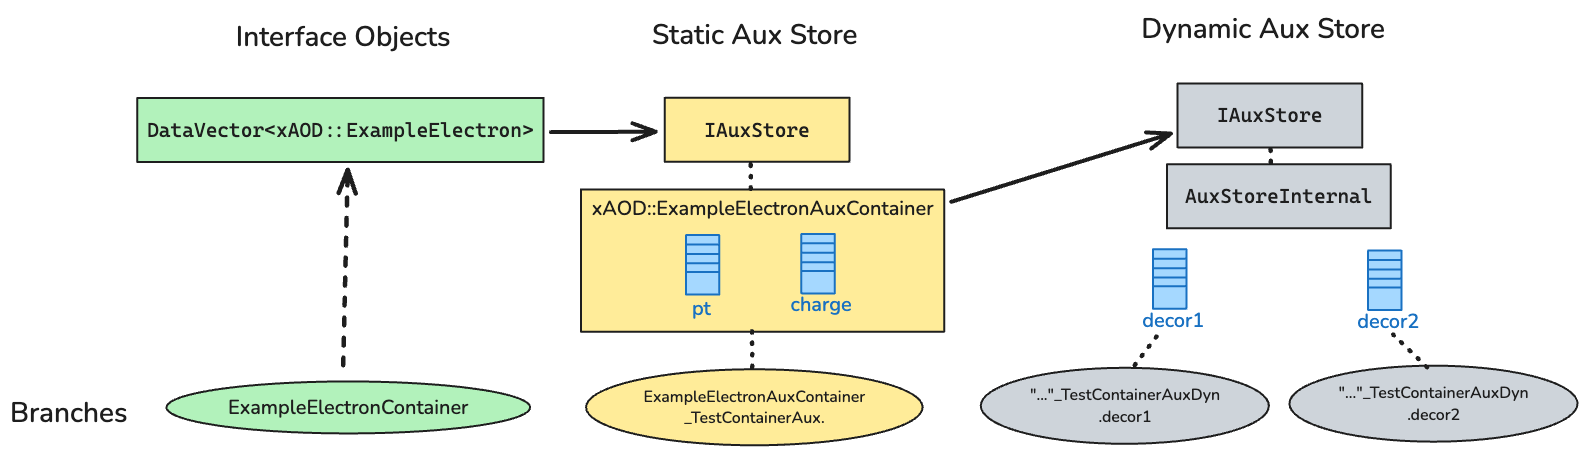
\includegraphics[width=\textwidth]{content/img/aux_store_better.png}
    \caption{The framework between interface objects and the static/dynamic auxiliary data store for a collection of xAOD::ExampleElectrons.}
    \label{fig:Mod_utests_aux_store}
\end{figure}





\section{Unit Tests}
\label{sec:Mod_utests_CI}
Unit tests are programs that act as a catch during the continuous integration of a codebase and test features that need to remain functional. 
Athena has a number of unit tests that check every merge request and nightly build for issues in the new code that could break core functionality, either at the level of Athena, ROOT, or any other software in the LCG stack.
There were no unit tests in the appropriate packages to handle selection of dynamic attributes, or decorations, on xAOD objects created during writing and read back.
To address this, a new xAOD test object needed to be created and written during a new unit test that fit into the existing unit tests.
The list of AthenaPoolExample unit tests that are currently executed during a nightly build can be found in Table \ref{tab:CI_Unit_Tests}.
These tests are executed in this order, as the objects created in one might be used in proceeding test.

\begin{table}[h]
    \centering
    \resizebox{\textwidth}{!}{
    \begin{tabular}{|c|c|c|}
        \hline
        $\textbf{Unit Test}$ & $\textbf{Employed Algorithms}$ & $\textbf{Function} (\text{Object Read}) \left[\text{Object Written}\right]$ \\
        \hline
      Write & WriteData & $\left[\text{ExampleHit}\right]$\\
        \hline
        ReadWrite & ReadData, ReWriteData & ($\text{ExampleHit}$), $\left[\text{ExampleTrack}\right]$\\
        \hline
        Read & ReadData & ($\text{ExampleHit}$)\\
        \hline
        Copy & None & $\textbf{Copies a file}$\\
        \hline
        ReadWriteNext & ReadData, ReWriteData & ($\text{ExampleHit}$, EventInfo), $\left[\text{ExampleTrack}\right]$ \\
        \hline
      *WritexAODElectron & ReadData, WriteExampleElectron & ($\text{ExampleTrack}$), $\left[xAOD::ExampleElectrons, decorations \right]$ \\
        \hline
        *ReadxAODElectron & ReadExampleElectron & (xAOD::ExampleElectrons, decorations) \\
        \hline
    \end{tabular}
    }
    \caption{List of unit tests in the AthenaPoolExample package that are currently executed during a nightly build. The unit tests marked by the `*' are the tests produced for this thesis.}
    \label{tab:CI_Unit_Tests}
\end{table}

The mechanism for passing a unit test is done automatically by building the framework, running the unit tests, and comparing the diff of the output file to the unit test with a reference file associated with that particular unit test. 
If the unit test passes, then the diff, a product of the \verb|git diff| command, will be empty and the unit test will be marked as passing.
Conversely, if the unit test fails, then the diff will be non-empty and the unit test will be marked as failing.

\subsection{WritexAODElectron.py}
The two new tests added to the package were \verb|WritexAODElectron| and \verb|ReadxAODElectron|.
During this first unit test, the first algorithm called is to \verb|ReadData| which reads off all of the \verb|ExampleTrack| objects stored in one of the files produced by the \verb|ReadWrite| unit-test.
Within the python script of the first unit test, the user is able to decide what decorations to have written to file. 
This is a part of the \verb|OutputStreamCfg| parameter, \verb|ItemList|, wherein the user specifies the object and its name in the format shown in Figure \ref{fig:Mod_utests_WritexAODElectron_ItemList}. 
\begin{figure}[h]
\centering
\begin{lstlisting}[language=C]
ItemList = [ "ExampleTrackContainer#MyTracks", 
"xAOD::ExampleElectronContainer#TestContainer",
"xAOD::ExampleElectronAuxContainer#TestContainerAux.-decor2"] )
\end{lstlisting}
\caption{WritexAODElectron ItemList for the OutputStreamCfg parameter. Showing how to select dynamic attributes at the CA level.}
\label{fig:Mod_utests_WritexAODElectron_ItemList}
\end{figure}



%% WriteExampleElectronAlgorithm
% Header (.h)
% Much of the code in Athena practice header/source-file separation, the header acting as an interface for the whole object and the source file containing the core functionality of the algorithm.
The header file includes various packages needed by the algorithm, such as data objects, \verb|Write/ReadHandleKeys|, base algorithms that give consistent structure to the algorithm, and whatever else is required. 
In the write-algorithm, there are \verb|ReadHandleKeys| for \verb|ExampleTrack| objects saved by a prior unit test. 
For the \verb|WriteHandleKeys|, there is one for the \verb|ExampleElectronContainer| and the name given to it is ``TestContainer". 
This ``TestContainer" name will be needed for the \verb|ReadExampleElectron| algorithm as the name is how it's able to refer to the correct \verb|ExampleElectronContainer| present in the input file. 
Additionally, a \verb|WriteHandleDecorKey| for the decoration objects is needed for appending each decoration onto each \verb|ExampleElectron| object. 
Figure \ref{fig:Mod_utests_WritexAODElectron_header} shows the syntax for how these keys would be presently defined.

\begin{figure}[h]
\centering
\begin{lstlisting}[language=C]
// Read key ExampleTracks
SG::ReadHandleKey<ExampleTrackContainer> m_exampleTrackKey{
    this, "ExampleTrackKey", "MyTracks"};  

// Write key for the ExampleElectronContainer
SG::WriteHandleKey<xAOD::ExampleElectronContainer>
    m_exampleElectronContainerKey{this, "ExampleElectronContainerName",
                                "TestContainer"};

// Decoration keys
SG::WriteDecorHandleKey<xAOD::ExampleElectronContainer> m_decor1Key{
    this, "ExampleElectronContainerDecorKey1", "TestContainer.decor1",
    "decorator1 key"};
SG::WriteDecorHandleKey<xAOD::ExampleElectronContainer> m_decor2Key{
    this, "ExampleElectronContainerDecorKey2", "TestContainer.decor2",
    "decorator2 key"};
\end{lstlisting}
\caption{WriteExampleElectronheader file setup}
\label{fig:Mod_utests_WritexAODElectron_header}
\end{figure}

% Source File (.c)
Then the \verb|WriteExampleElectron| algorithm is called and takes \verb|ExampleTracks|, creates an \verb|ExampleElectron| object and sets the electrons \verb|pt| to the tracks \verb|pt|. 
\begin{figure}[h]
\centering
\begin{lstlisting}[language=C]
auto elecCont = std::make_unique<xAOD::ExampleElectronContainer>();
auto elecStore = std::make_unique<xAOD::ExampleElectronAuxContainer>();
elecCont->setStore(elecStore.get());

SG::ReadHandle<ExampleTrackContainer> trackCont(m_exampleTrackKey, ctx);
elecCont->push_back(std::make_unique<xAOD::ExampleElectron>());

for (const ExampleTrack* track : *trackCont) {
    // Take on the pT of the track
    elecCont->back()->setPt(track->getPT());
}

SG::WriteHandle<xAOD::ExampleElectronContainer> objs(m_exampleElectronContainerKey, ctx);
ATH_CHECK(objs.record(std::move(elecCont), std::move(elecStore)));
\end{lstlisting}
\caption{Algorithm to initialize and write T/P data (ExampleTracks) to an xAOD object container (ExampleElectronContainer).}
\label{fig:Mod_utests_WritexAODElectron1}
\end{figure}
As shown in Figure \ref{fig:Mod_utests_WritexAODElectron1}, the \verb|ExampleElectronContainer| and \verb|ExampleElectronAuxContainer| are created and set to the \verb|elecCont| and \verb|elecStore| respectively.
The \verb|elecCont| has an associated aux store, so the \verb|setStore| function is called with the \verb|elecStore| pointer.
The track container is accessed by using StoreGate's \verb|ReadHandle|, which associates the \verb|m_exampleTrackKey| with the \verb|ExampleTrackContainer| specified in the header file.
This is then looped over all elements in the container and the \verb|pt| of each track is set to the \verb|pt| of the electron.
A \verb|WriteHandle|, called \verb|objs|, is then created for the container of \verb|ExampleElectrons| which is then recorded.

Within the same algorithm, the next step is to loop over each of the newly produced \verb|ExampleElectrons|, accessing the decorations \verb|decor1| and \verb|decor2|, and setting each to an arbitrary float value that are easily identifiable later.
Figure \ref{fig:Mod_utests_WritexAODElectron2} shows how this is done using two handles for each decoration. 
Note the difference here using the \verb|WriteDecorHandle|, where the prior handle type was \verb|WriteHandle|.
\begin{figure}[h]
    \centering
\begin{lstlisting}[language=C]
SG::WriteDecorHandle<xAOD::ExampleElectronContainer, float> hdl1(m_decor1Key,ctx);
SG::WriteDecorHandle<xAOD::ExampleElectronContainer, float> hdl2(m_decor2Key,ctx);

for (const xAOD::ExampleElectron* obj : *objs) {
    hdl1(objs) = 123.;
    hdl2(objs) = 456.;
}
\end{lstlisting}
    \caption{Writing of dynamic variables for each of the ExampleElectron objects.}
    \label{fig:Mod_utests_WritexAODElectron2}
\end{figure}


\subsection{ReadxAODElectron.py}
The only algorithm called in this test is \verb|ReadExampleElectron|.
The header file for the \verb|ReadExampleElectron| only creates \verb|ReadHandleKey| for the container of ExampleElectrons, with the same name from the header of the \verb|WriteExampleElectron| algorithm header, syntax shown in Figure \ref{fig:Mod_utests_ReadxAODElectron1}.
\begin{figure}[h]
    \centering
\begin{lstlisting}[language=C]
SG::ReadHandleKey<xAOD::ExampleElectronContainer>
m_exampleElectronContainerKey{this, "ExampleElectronContainerName",
                                "TestContainer"};
\end{lstlisting}
    \caption{ReadHandleKey for the container of ExampleElectrons}
    \label{fig:Mod_utests_ReadxAODElectron1}
\end{figure}
From the source file, we can initialize the \verb|ReadHandleKey| object by a simple \verb|ATH_CHECK(m_exampleElectronContainerKey.initialize());| in the \verb|initialize()| method.
This allows for, when defining the \verb|ReadHandle| in execute, identifying the correct container defined in the header file.
The same can be done for the decoration key, which needs a separate read handle, \verb|ReadDecorHandle|. 
Once this is setup, all the read algorithm needs to do is to loop over all the \verb|ExampleElectrons| in the ``TestContainer" and access their $p_T$ and charge.

\section{Results}
This project sought to replace existing unit tests that created \verb|ExampleHits|, T/P EDM objects, to be written and read back. 
An independent xAOD object, \verb|ExampleElectron|, was created and implemented into two new unit tests that write and read \verb|ExampleElectron| objects along with their chosen dynamic attributes. 
A merge request was created, approved, and merged into the Athena software framework.
Future work can be done to fully modernize the package these unit tests reside, \verb|AthenaPoolExampleAlgorithms|, including unit tests that test core functionality of AthenaMT/AthenaMP, and newer storage formats like RNTuple. 

%---

%---
% 6. Conclusion
% -- 
\chapter{Conclusion}
The work done for this thesis was primarily motivated to find avenues to optimize resource usage for GRID I/O operations. 
The toy model testing allowed us to create branches with data similar compression ratios to real and simulated data, allowing to investigate the hypothesis that modifying the basket buffer limit had an effect on disk and memory usage.
It led to the conclusion that, upon investigating with real data and real MC simulation, that there might be an avenue to look at both ROOT and Athena to limit basket sizes. 

% Recap what Chapter 4 said into 1-2 sentences
% What was the conclusion to the toymodel/basket-size modifications to the derivation jobs? 
Modifying the basket buffer sizes at the Athena level shows there was a balance was struck when using the Athena basket buffer size limited to 128 kB between memory-usage and the size of the DAOD to be saved long-term. 
Removing the basket buffer size limit, the $5.5 \%$ saving in PHYSLITE MC disk-usage at the expense of an $11 \%$ increase in memory-usage could be a trade-off worth making in some scenarios. 
A class of potentially unoptimized AOD branches in MC simulated data was also brought to light during this study.
The leading indicator to potential optimization is the highly compressible nature of these branches post-derivation.
Further work could be done to look into these AOD branches to identify areas where further work can be done to reduce the overall AOD footprint. 

% Recap Chapter 5 into 1-2 sentences. 
The xAOD EDM comes with a number of new additions to bring about optimization the future of analysis work at the ATLAS experiment.
Integrating the new features into a few comprehensive unit tests allow for the nightly CI builds to catch any issues that break core I/O functionality as it pertains to the xAOD EDM, which has not been done before.
These new unit-tests exercise reading and writing select decorations ontop of the already existing data structures attached to an example object called \verb|ExampleElectron|. 


%---



% ===== PRINT BIBLIOGRAPHY =====  

\begingroup
\setstretch{1}
\setlength\bibitemsep{20pt}
\addcontentsline{main.toc}{chapter}{REFERENCES}
\printbibliography[
    heading=bibintoc,
    title={REFERENCES}
]
\endgroup
%-------------------------------------------------------------------------------
\clearpage
\appendix

% \chapter{Toy Model AOD Code}
% \section{Athena job configuration example}
A general Athena application using \verb|ComponentAccumulator| written in pseudocode would take the form: 
\begin{lstlisting}[language=Python]
    # Import Packages
    from AthenaConfiguration.AllConfigFlags import initConfigFlags
    from AthenaConfiguration.ComponentFactory import CompFactory
    from OutputStreamAthenaPool.OutputStreamConfig import OutputStreamCfg, outputStreamName

    outputStreamName = "StreamA"
    outputFileName = "output.root"

    # Setup flags
    flags = initConfigFlags()
    flags.Input.Files = ["input.root"]
    flags.addFlag(f"Output.{streamName}FileName", outputFileName)
    flags.lock()

    # Main Service(s)
    from AthenaConfiguration.MainServicesConfig import MainServicesCfg
    acc = MainServicesCfg( flags )

    # Add algorithms to the accumulator
    acc.addEventAlgo( CompFactory.MyAlgorithm(MyParameters) )

    import sys
    sc = acc.run(flags.Exec.MaxEvents)
\end{lstlisting}

The \verb|acc| is the \verb|ComponentAccumulator|, so here the user might have more than one Algorithm it needs to call, but each one would have a separate \verb|.addEventAlgo| call. 
When \verb|flag.lock()| is called, any previously established flags will be set in place and unable to be changed. 

\chapter{Derivation Production Data}
\section{Derivation production datasets} 
\label{app: deriv job dataset}


For both the nightly and the release testing, the data derivation job, which comes from the dataset 

\lstinputlisting{content/dataset-data.txt}

was ran with the input files 

\lstinputlisting{content/inputfiles-data.txt}

Similarly, the MC derivation job, comes from the dataset 

\lstinputlisting{content/dataset-mc.txt}

was ran with input files

\lstinputlisting{content/inputfiles-mc.txt}


\chapter{Athena Configuration Job} \label{app:athena-job-config}
\section{Athena job configuration example}

An Athena job configuration is a script that allows the user to steer a specific program in the framework.
Steering allows one to, at a high-level, configure low-level behavior of any kind of production job. 
A general Athena application using \verb|ComponentAccumulator| written in pseudocode would take the form: 
\begin{lstlisting}[language=Python]
    # Import Packages
    from AthenaConfiguration.AllConfigFlags import initConfigFlags
    from AthenaConfiguration.ComponentFactory import CompFactory
    from OutputStreamAthenaPool.OutputStreamConfig import OutputStreamCfg, outputStreamName

    # Configure Output
    outputStreamName = "StreamA"
    outputFileName = "output.root"

    # Setup flags
    flags = initConfigFlags()
    flags.Input.Files = ["input.root"]
    flags.addFlag(f"Output.{streamName}FileName", outputFileName)
    flags.lock()

    # Main Service(s)
    from AthenaConfiguration.MainServicesConfig import MainServicesCfg
    acc = MainServicesCfg( flags )

    # Add algorithms to the accumulator
    acc.addEventAlgo( CompFactory.MyAlgorithm(MyParameters) )

    # Run
    import sys
    sc = acc.run(flags.Exec.MaxEvents)
\end{lstlisting}

The \verb|acc| is the \verb|ComponentAccumulator|, so here the user might have more than one Algorithm it needs to call, but each one would have a separate \verb|.addEventAlgo| call. 
When \verb|flag.lock()| is called, any previously established flags will be set in place and unable to be changed. 


\end{document}
